\subsection{\tty production Measurement}
\label{sec:tty_prod_measurement}
%\textcolor{red}{To do: add results for inclusive \tty measurement (\tty production + decay), ongoing since the particle level information of \tty decay was missing until recently.}

This section presents the results of the unfolded likelihood fit to the real data for the \tty production cross section measurement. Profile likelihood unfolding method is performed to measure the cross-section from the data. %(at this point the profile likelihood unfolding shold be clear to the reader, ehcke that it is properly explaine in the section) 
After the fit, the fitted values of the POIs are shown in \cref{fig:pt_unfolded_ljet_table_realdata} and \cref{fig:pt_unfolded_dilep_table_realdata} for single lepton channel and dilepton channel respectively. Using measured POIs, the post-fit distributions at reconstruction level are shown in \cref{fig:pt_postfit_ljet_realdata} for the single lepton channel and in \cref{fig:pt_postfit_dilep_realdata} for the dilepton channel. The distributions are only shown for the observable $p_T(\gamma)$, rest are shown in the Appendix [ToDo].

As mentioned earlier that the systematic uncertainties are taken into account as the nuisance parameter (NP) in the likelihood function and they are kept constrained.
% explain pull plot
During the likelihood minimization, the shift in the fitted values for the NP are shown using the pull plot. Pull plot is used to visualize the difference between the measured values and the predicted values from a fit, normalized by the uncertainty. Each data point in a pull plot represents a particular NP. The x-value of the data point is the "pull" value, calculated as (measured - predicted) / uncertainty. If the fit is perfect, the pull values should follow a standard normal distribution (mean of 0 and standard deviation of 1). This is because the difference between the measured and predicted values should be zero on average, and the normalization by the uncertainty should scale the distribution to have a standard deviation of 1. The pull plots are shown in Figure ~\ref{fig:pull_plot_pt_tty_dec_free_ljet_mu_blinded}, Figure ~\ref{fig:pull_plot_pt_tty_dec_free_dilep_mu_blinded_1}, ~\ref{fig:pull_plot_pt_tty_dec_free_dilep_mu_blinded_2}. % explain the observation which NP are constrained and pulled and which are not
The pull is observed for \tty decay herwig7 variation as well as for 

The correlation is calculated among the POIs and the NPs shown in \cref{fig:NP-corr_ljet_mu_blinded} and in \cref{fig:NP-corr_dilep_mu_blinded}, for the single lepton and dilepton channels respectively. The post-fit value of all the NPs changed within 1 $\sigma$, with a large fraction of the NPs having very small pulls and constraints, which indicate that the fit is robust and not affected by any unexpected behavior of the NPs. Here constraint means that the pre-fit uncertainty for that parameter was overspecified,i.e., the actual post-fit uncertainty turned out to be smaller than the pre-fit estimate. % explain the observation which NPs are correlated and which are not

Also the impact of the NPs on the measurement of the POIs are estimated using the Ranking plot. 
% explain ranking plot
The ranking plot shows the impact of the NPs on the measurement of the POIs. The impact is calculated by varying each NP by $\pm 1 \sigma$ while keeping others at the post-fit vale and measuring the change in the POIs. Ranking plots are shown in Figures ~\ref{fig:ranking_ljet_total} and ~\ref{fig:ranking_dilep_total} for single lepton and dilepton channels. Furthermore the post-fitted values of the POIs (Norm Factors) are shown in Figures ~\ref{fig:pt_unfolded_ljet_table_realdata} and ~\ref{fig:pt_unfolded_dilep_table_realdata} for single lepton channel and dilepton channel respectively. % explain the observation which NPs are highly ranked and which are not

The unfolded distributions at particle level are shown in Figures ~\ref{fig:pt_unfolded_ljet_dist_realdata} and ~\ref{fig:pt_unfolded_dilep_dist_realdata_1} and ~\ref{fig:pt_unfolded_dilep_dist_realdata_2} for single lepton and dilepton channels. The normalized unfolded distributions are shown in Figures ~\ref{fig:tty_prod_diff_Ljets_norm} and ~\ref{fig:tty_prod_diff_DL1_norm} for single lepton and dilepton channels respectively. The decomposed uncertainties of the unfolded distributions for the absolute differential cross-sections are illustrated in Figures ~\ref{fig:tty_prod_diff_Ljets_groupedimpact} and ~\ref{fig:tty_prod_diff_DL1_groupedimpact}, ~\ref{fig:tty_prod_diff_DL2_groupedimpact} for single lepton channel and dilepton channel respectively. $\chi^2$/ndf and $p$-values between the measured absolute and normalised cross-sections of \tty production and the NLO \MGNLO simulations interfaced with \PYTHIA[8] and \HERWIG[7] are shown in Table ~\ref{tab:chi2_ttyprod}.


%The parameter of interests $\mu$ (\tty. prod signal strength) and the normalisation of \tty (decay) 
%blinded throughout the process. This means that the value of 
%this parameter will not be revealed until the end of the 
%analysis, ensuring a fair and unbiased evaluation of the 
%model's performance. The purpose of this approach is to 
%ensure that any potential biases or preconceptions do 
%not influence the interpretation of the results, while checking the behavior of the nuisance 
%parameters in the fit to the data. 



%the NPs are behaving as expected.  
%are robust and not affected by any unexpected behavior of the NPs.

%In summary, by keeping the POIs blinded throughout 
%the process, we have ensured a fair and unbiased 
%evaluation of the model's performance, and by studying 
%the behavior of the NPs, we have validated the 
%robustness of our results.

\begin{figure}[ht]
  \centering
  \subfloat[]{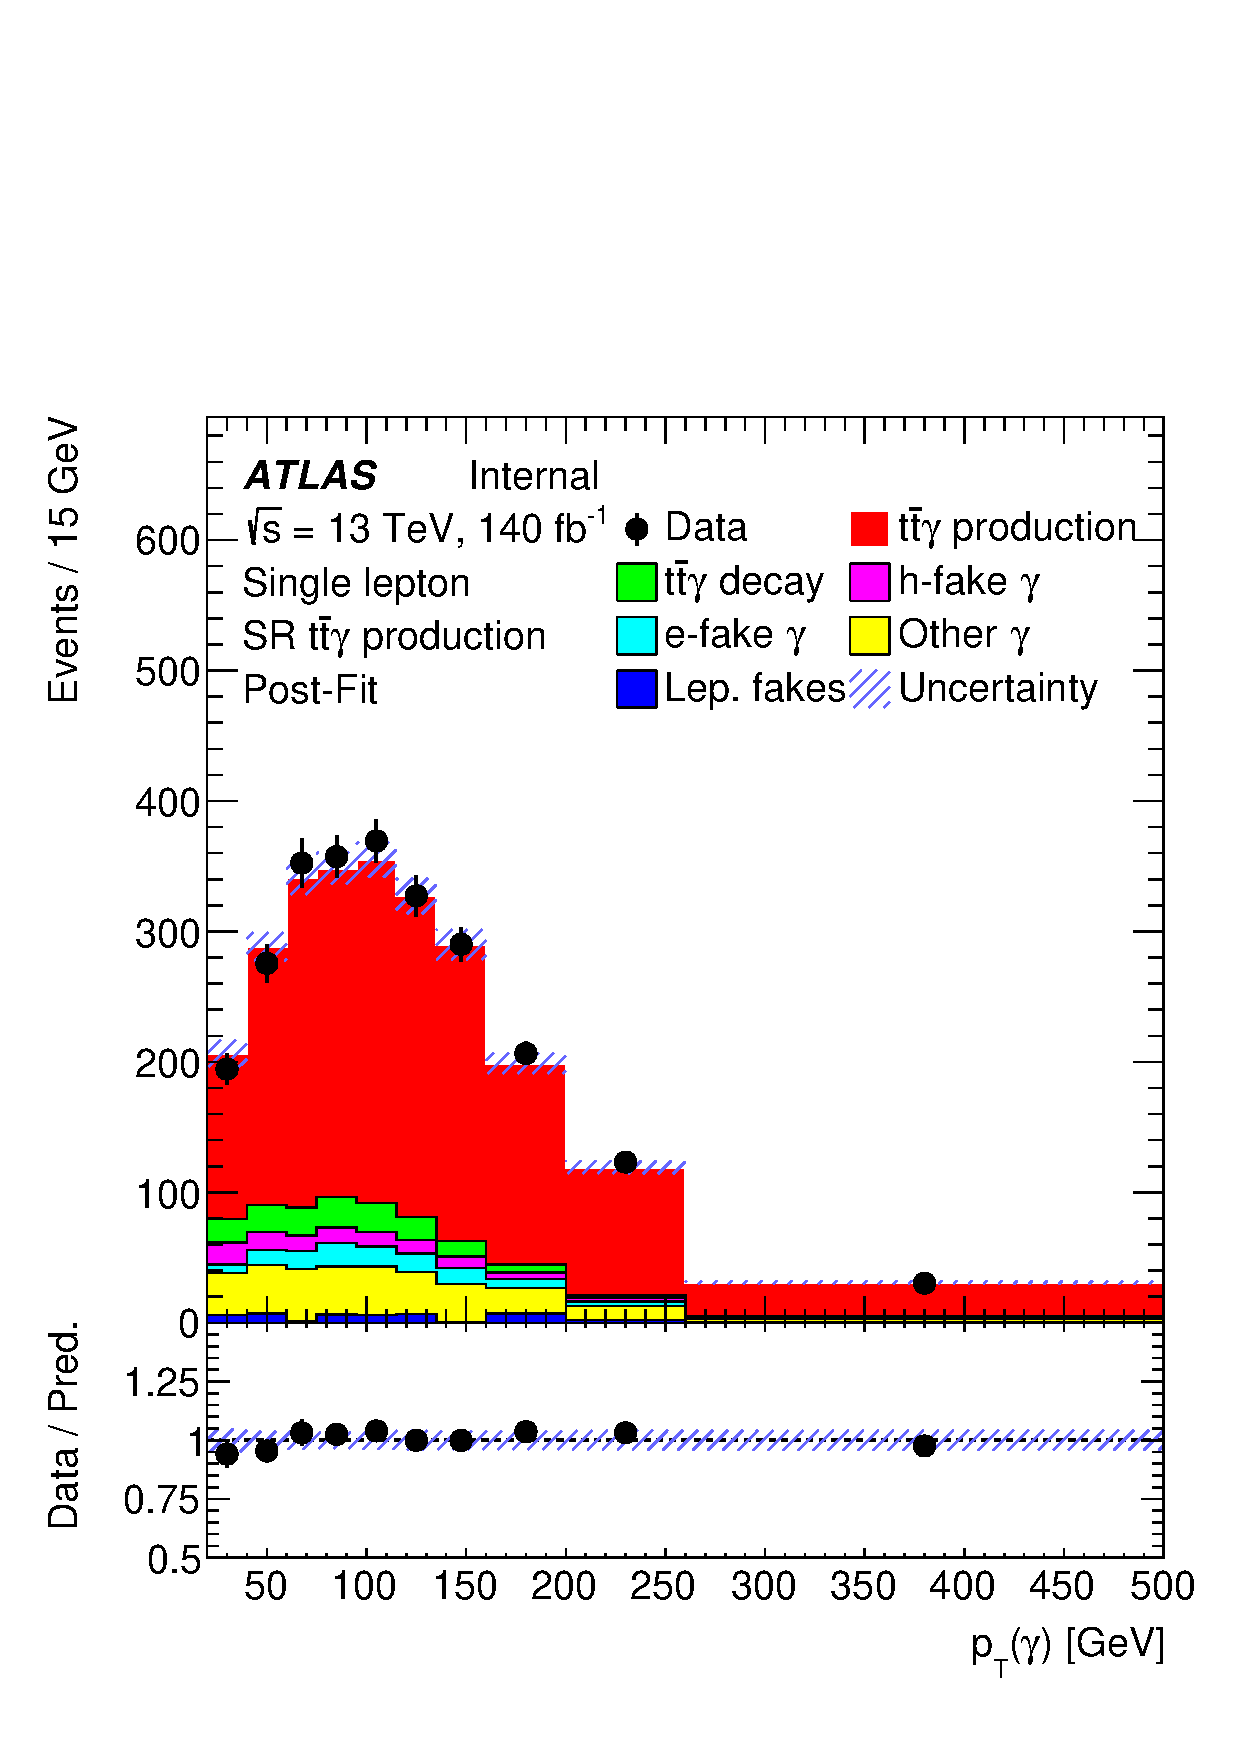
\includegraphics[width=0.30\textwidth]{figures/diff_xsec/ljet/post_fit/tty1l_pt_all_syst/Plots/SR1_postFit.pdf}}
  \quad \quad
  \subfloat[]{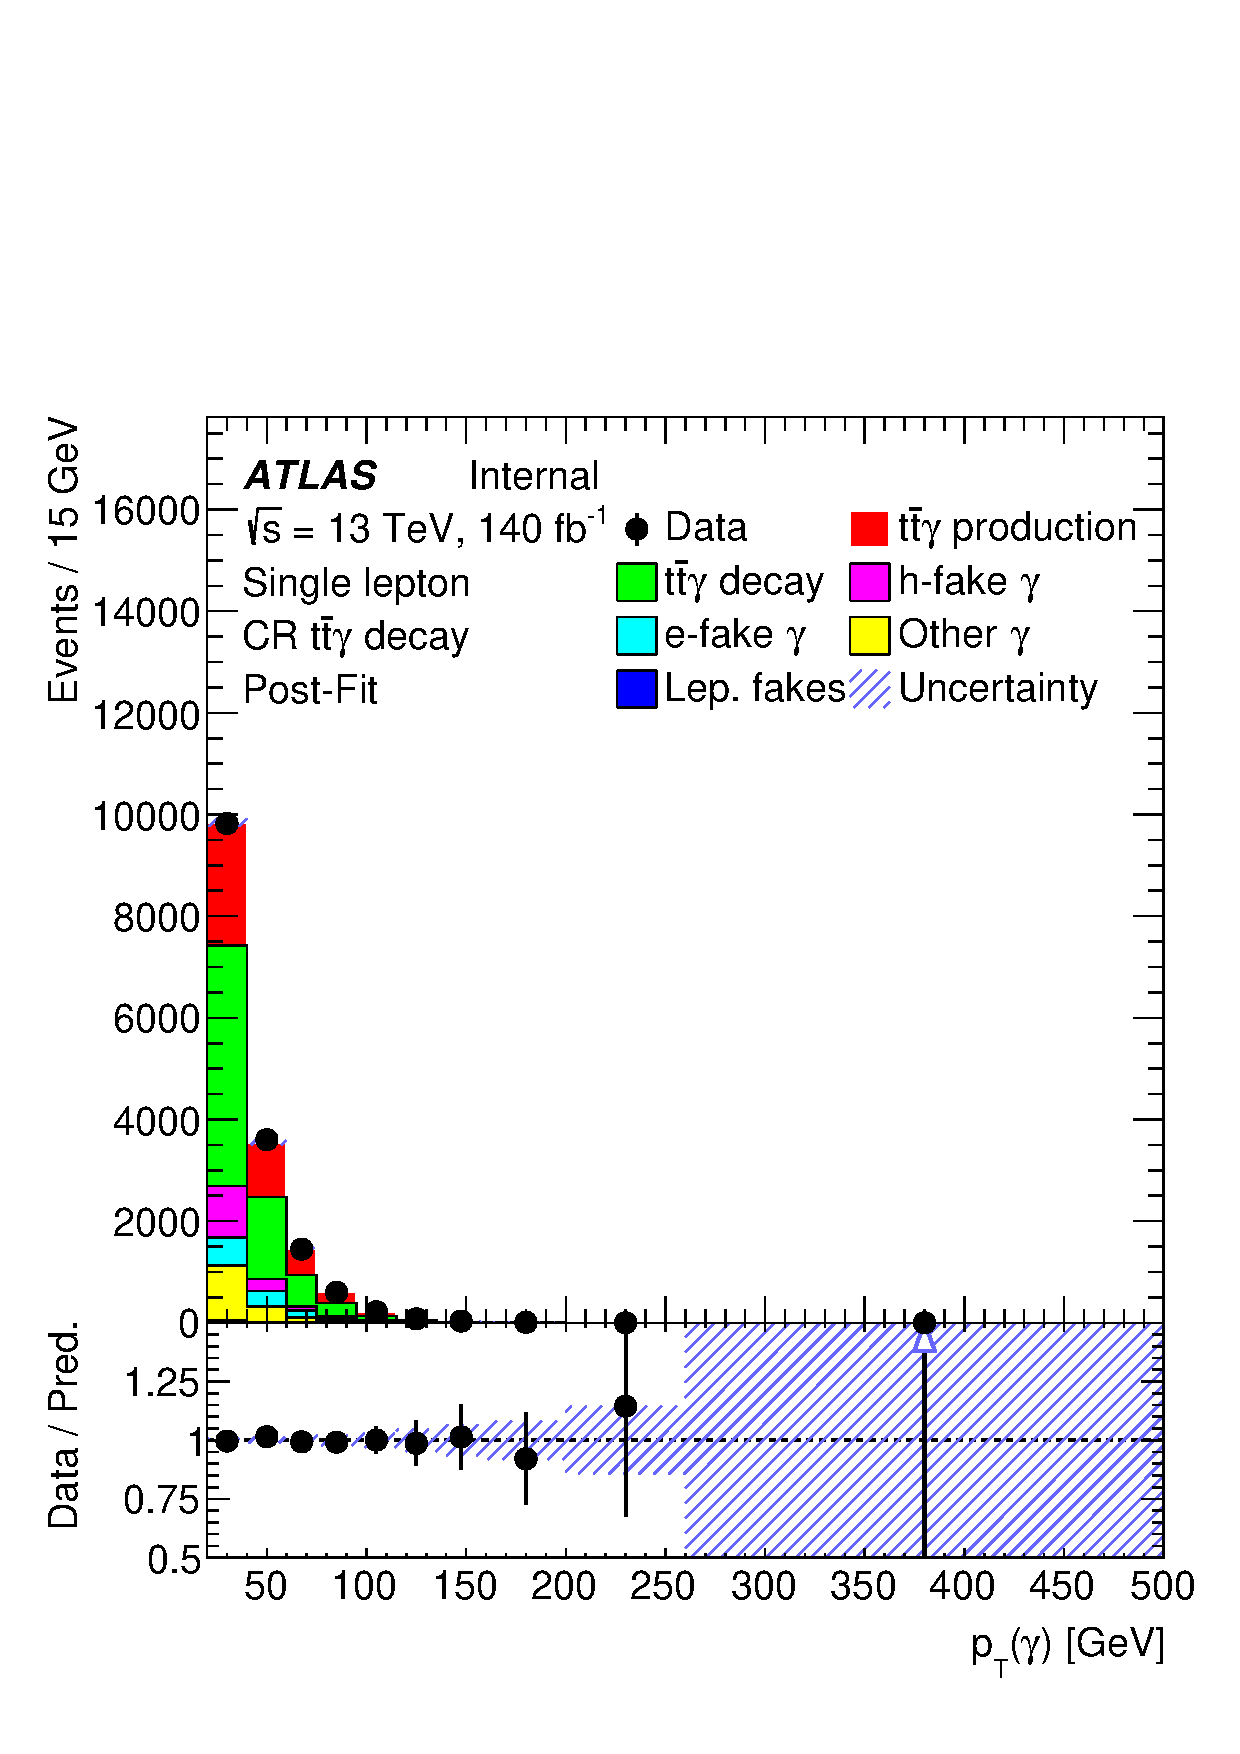
\includegraphics[width=0.30\textwidth]{figures/diff_xsec/ljet/post_fit/tty1l_pt_all_syst/Plots/SR2_postFit.pdf}}
  \quad \quad
  \subfloat[]{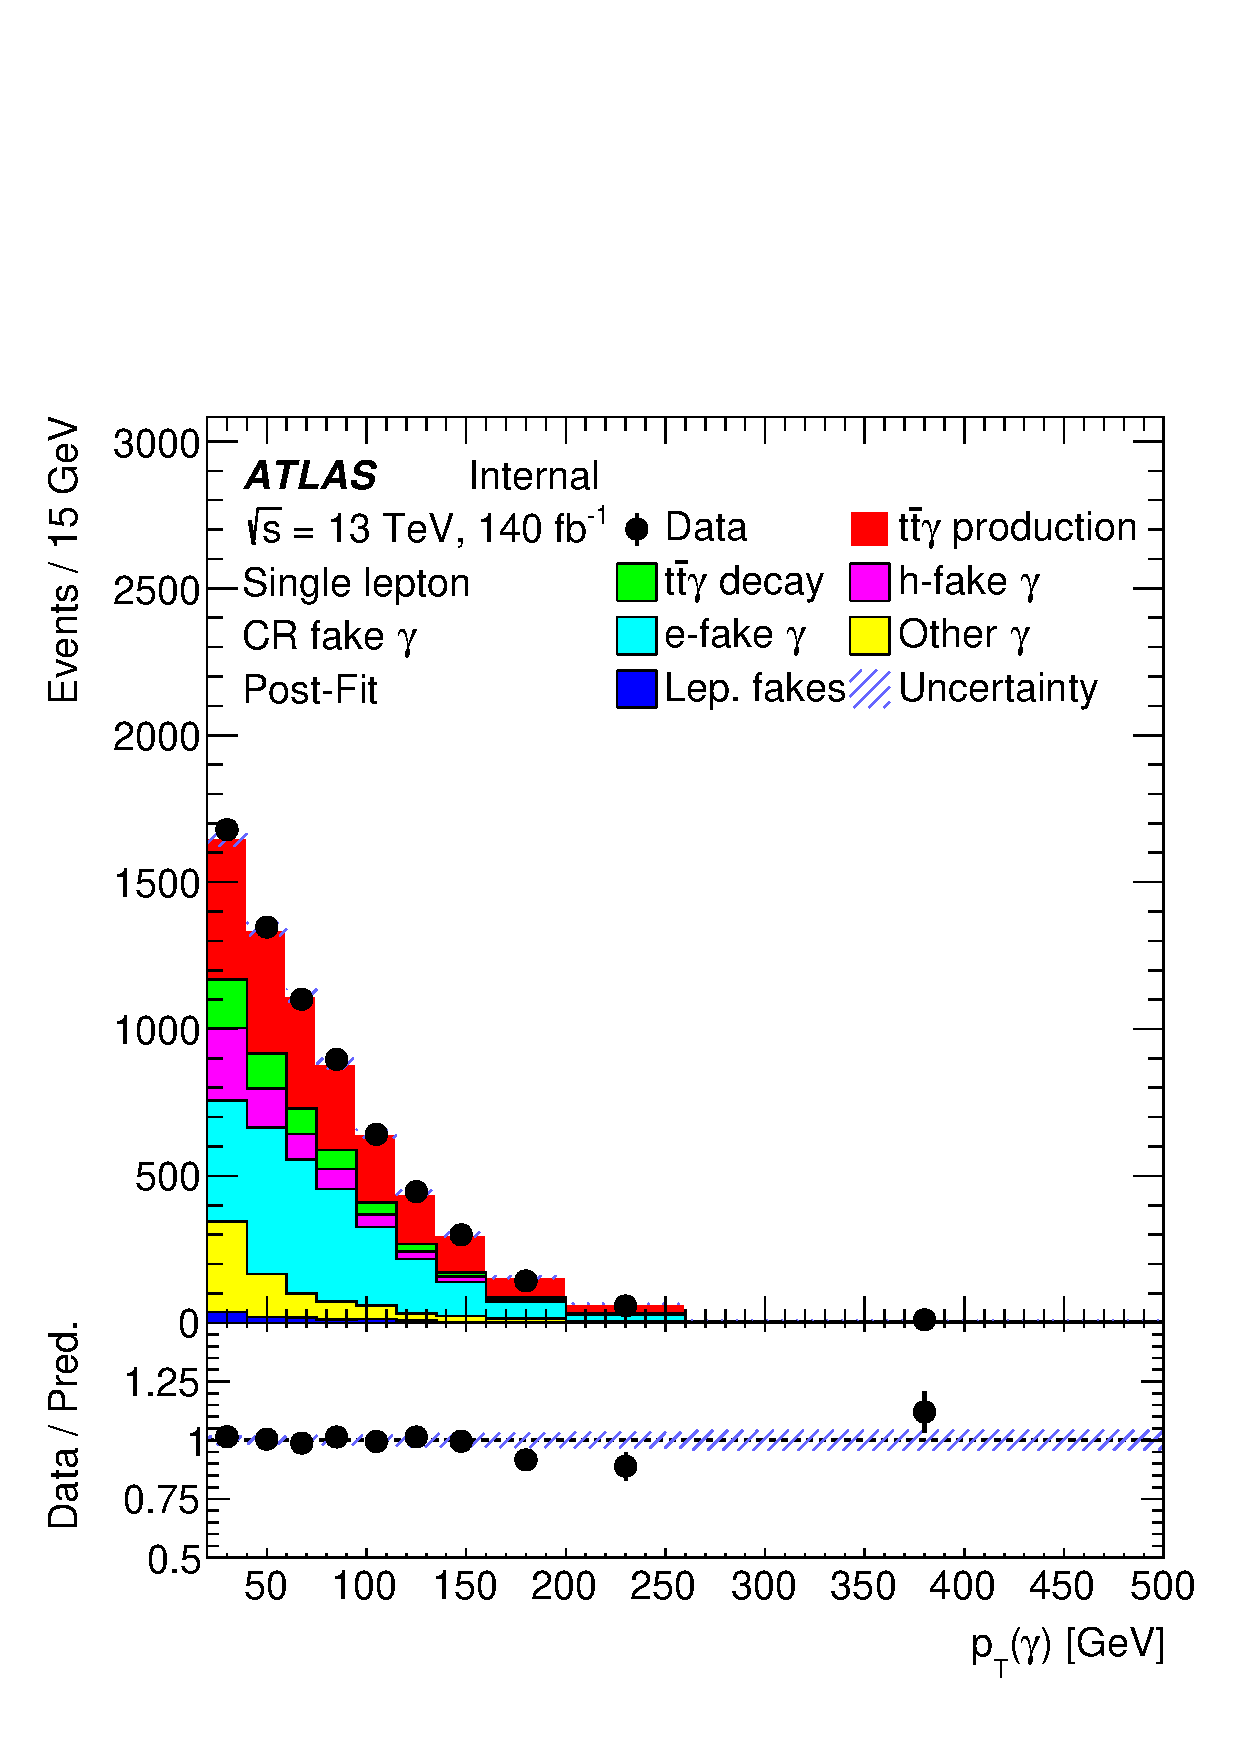
\includegraphics[width=0.30\textwidth]{figures/diff_xsec/ljet/post_fit/tty1l_pt_all_syst/Plots/SR3_postFit.pdf}}
  \quad \quad
  \subfloat[]{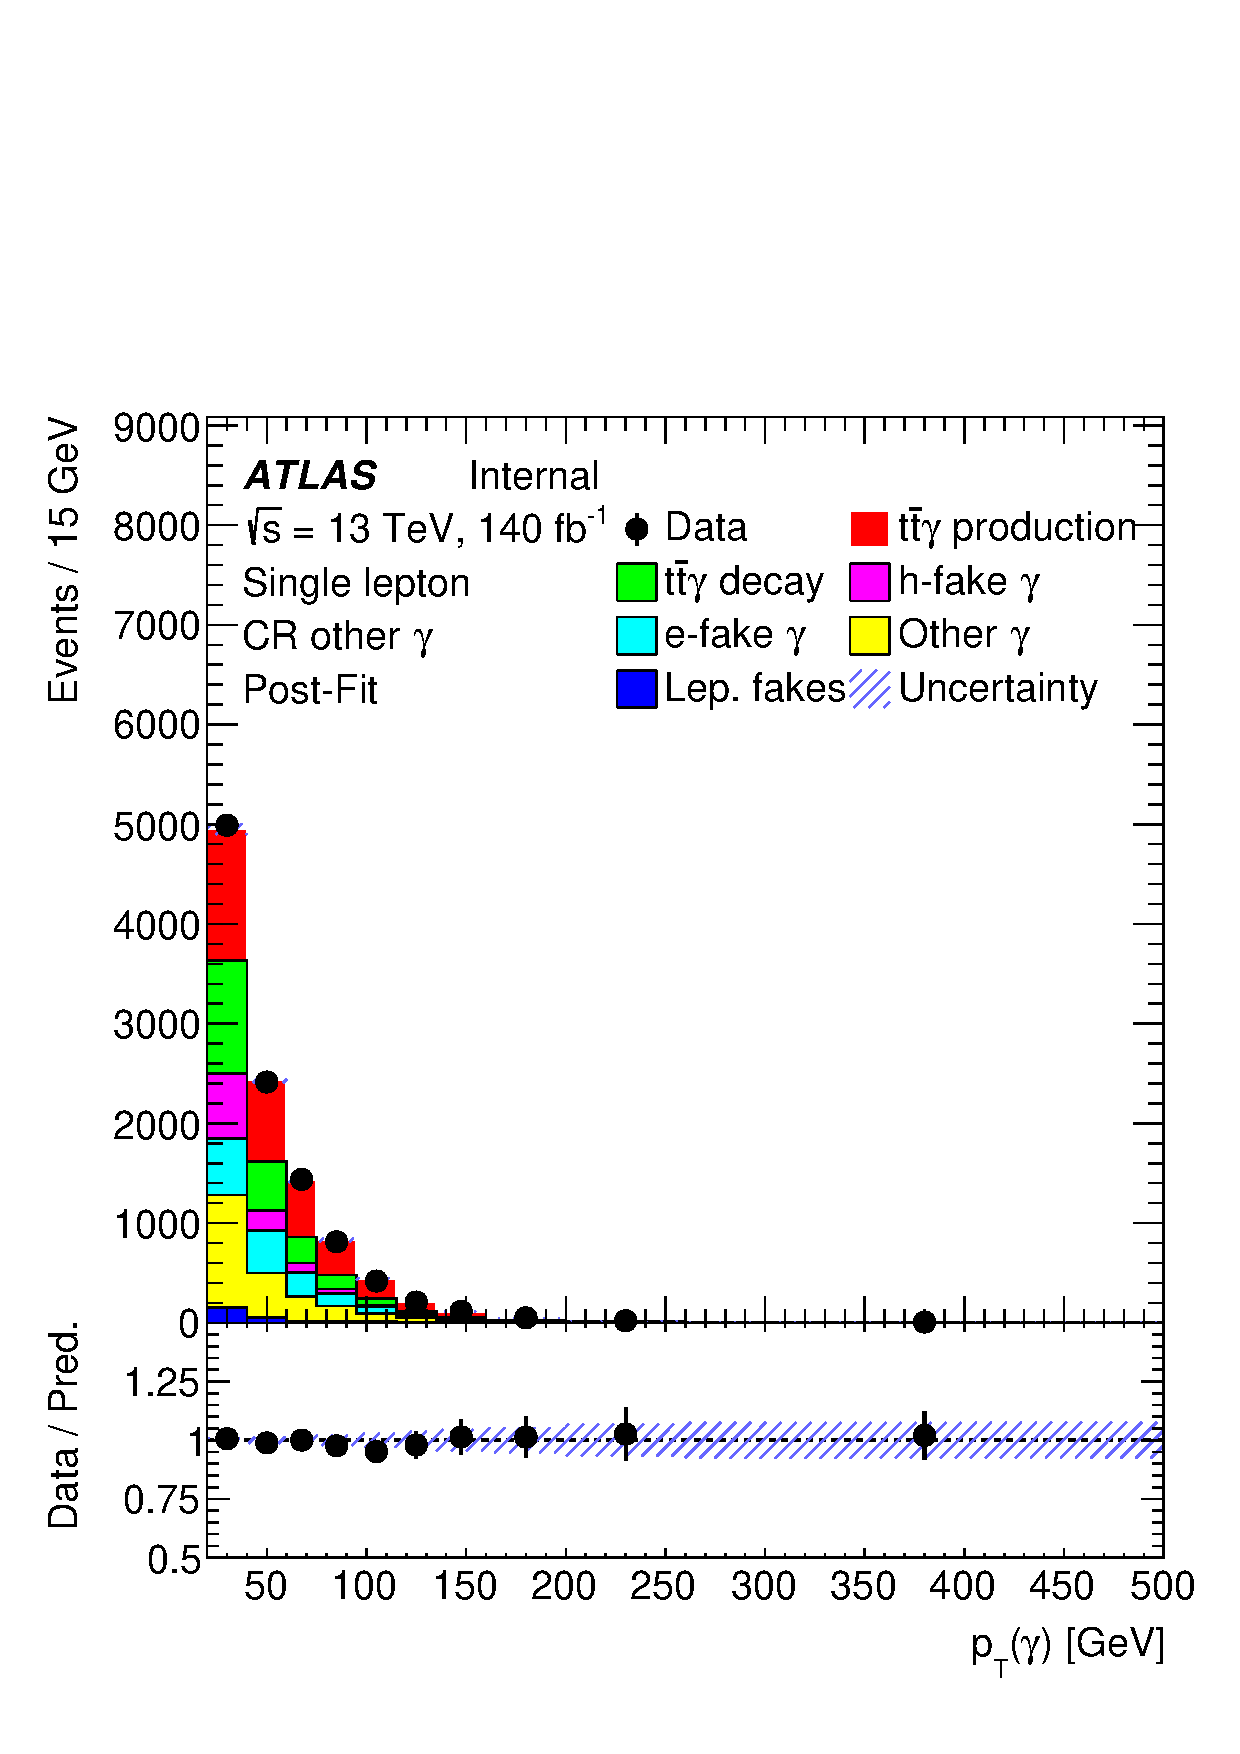
\includegraphics[width=0.30\textwidth]{figures/diff_xsec/ljet/post_fit/tty1l_pt_all_syst/Plots/SR4_postFit.pdf}}


  \caption{The post-fit distributions of $p_T(\gamma)$ in 4 regions ( (a) \tty (prod.) enriched region  (b) \tty (dec.) enriched region
  (c) fakes enriched region (d) prompt photon enriched region) in single lepton channel. }
  \label{fig:pt_postfit_ljet_realdata}
\end{figure}
\FloatBarrier


\begin{figure}[ht]
  \centering
  \subfloat[]{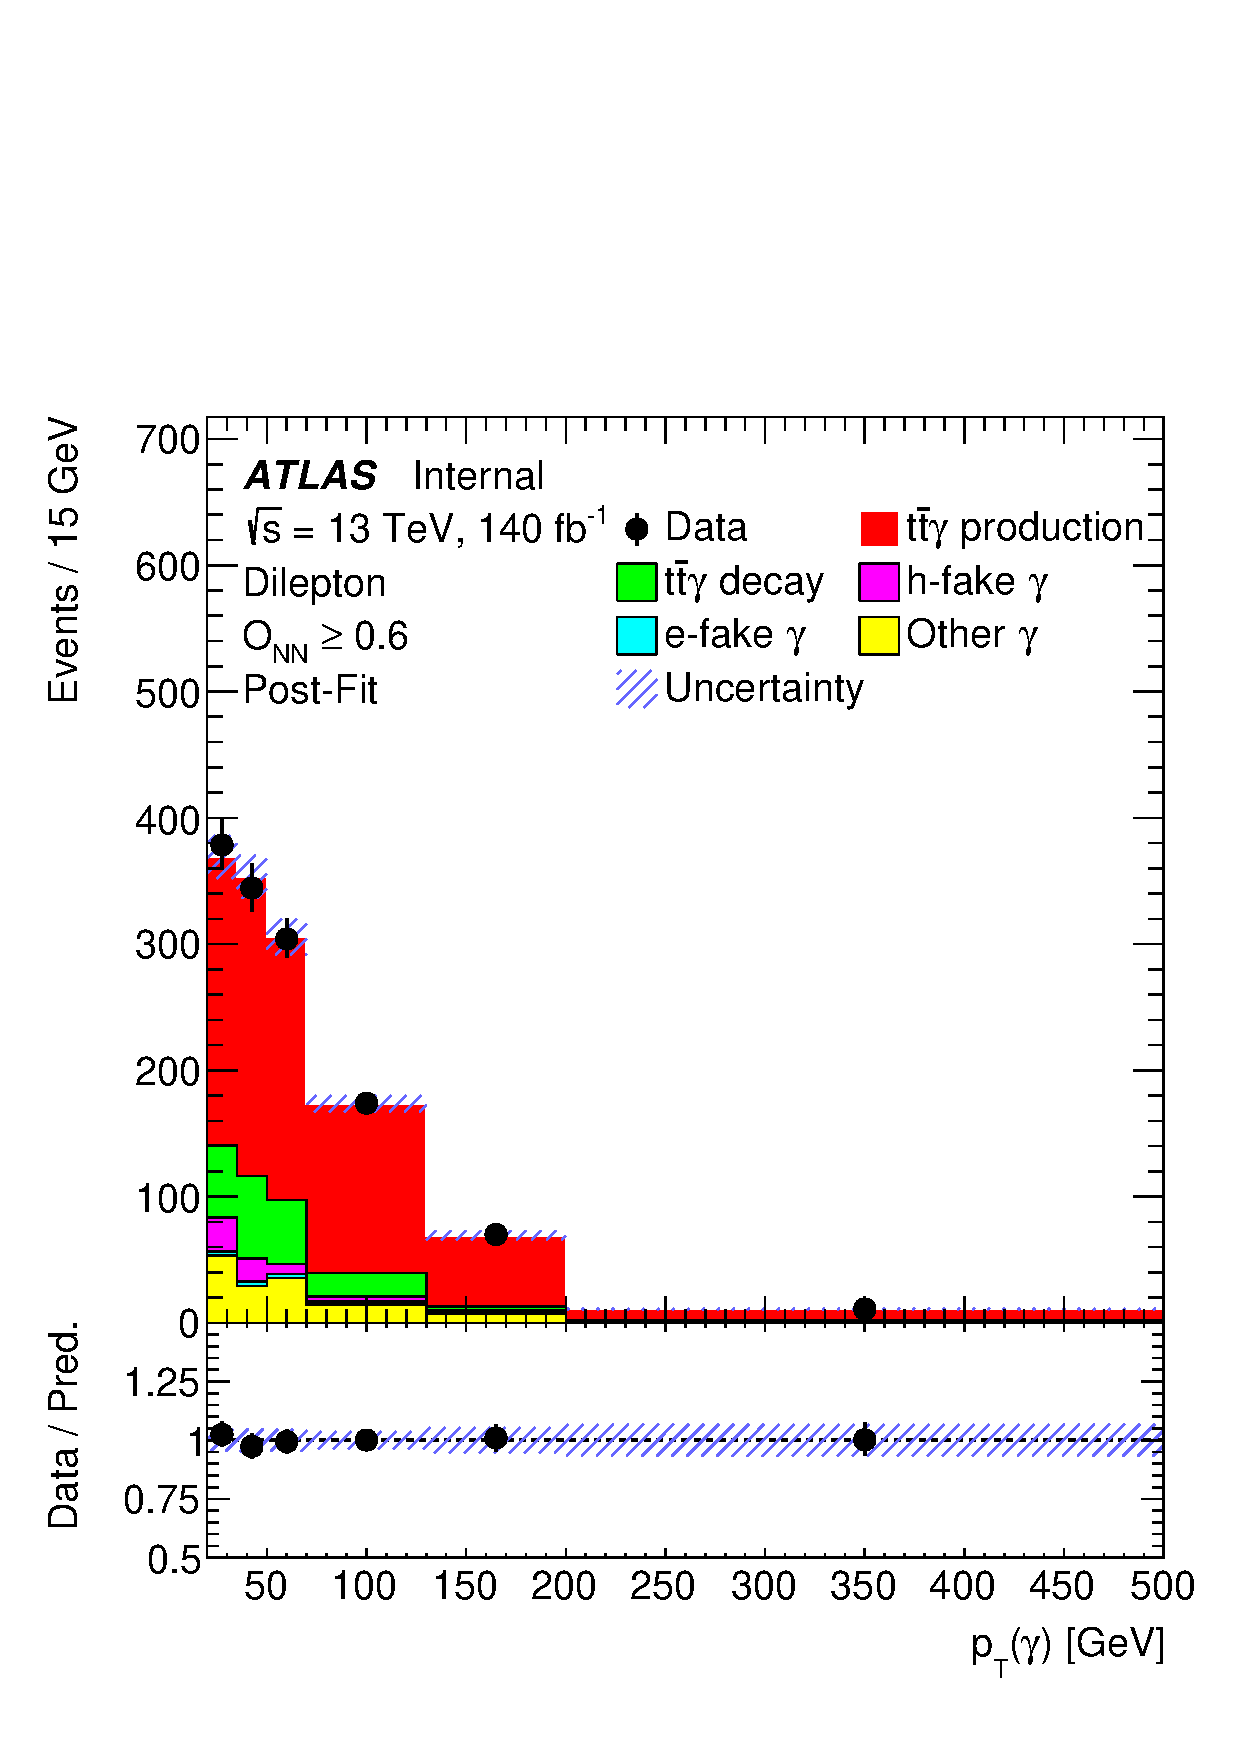
\includegraphics[width=0.30\textwidth]{figures/diff_xsec/dilep/post_fit/tty2l_pt_all_syst/Plots/SR1_postFit.pdf}}
  \quad \quad
  \subfloat[]{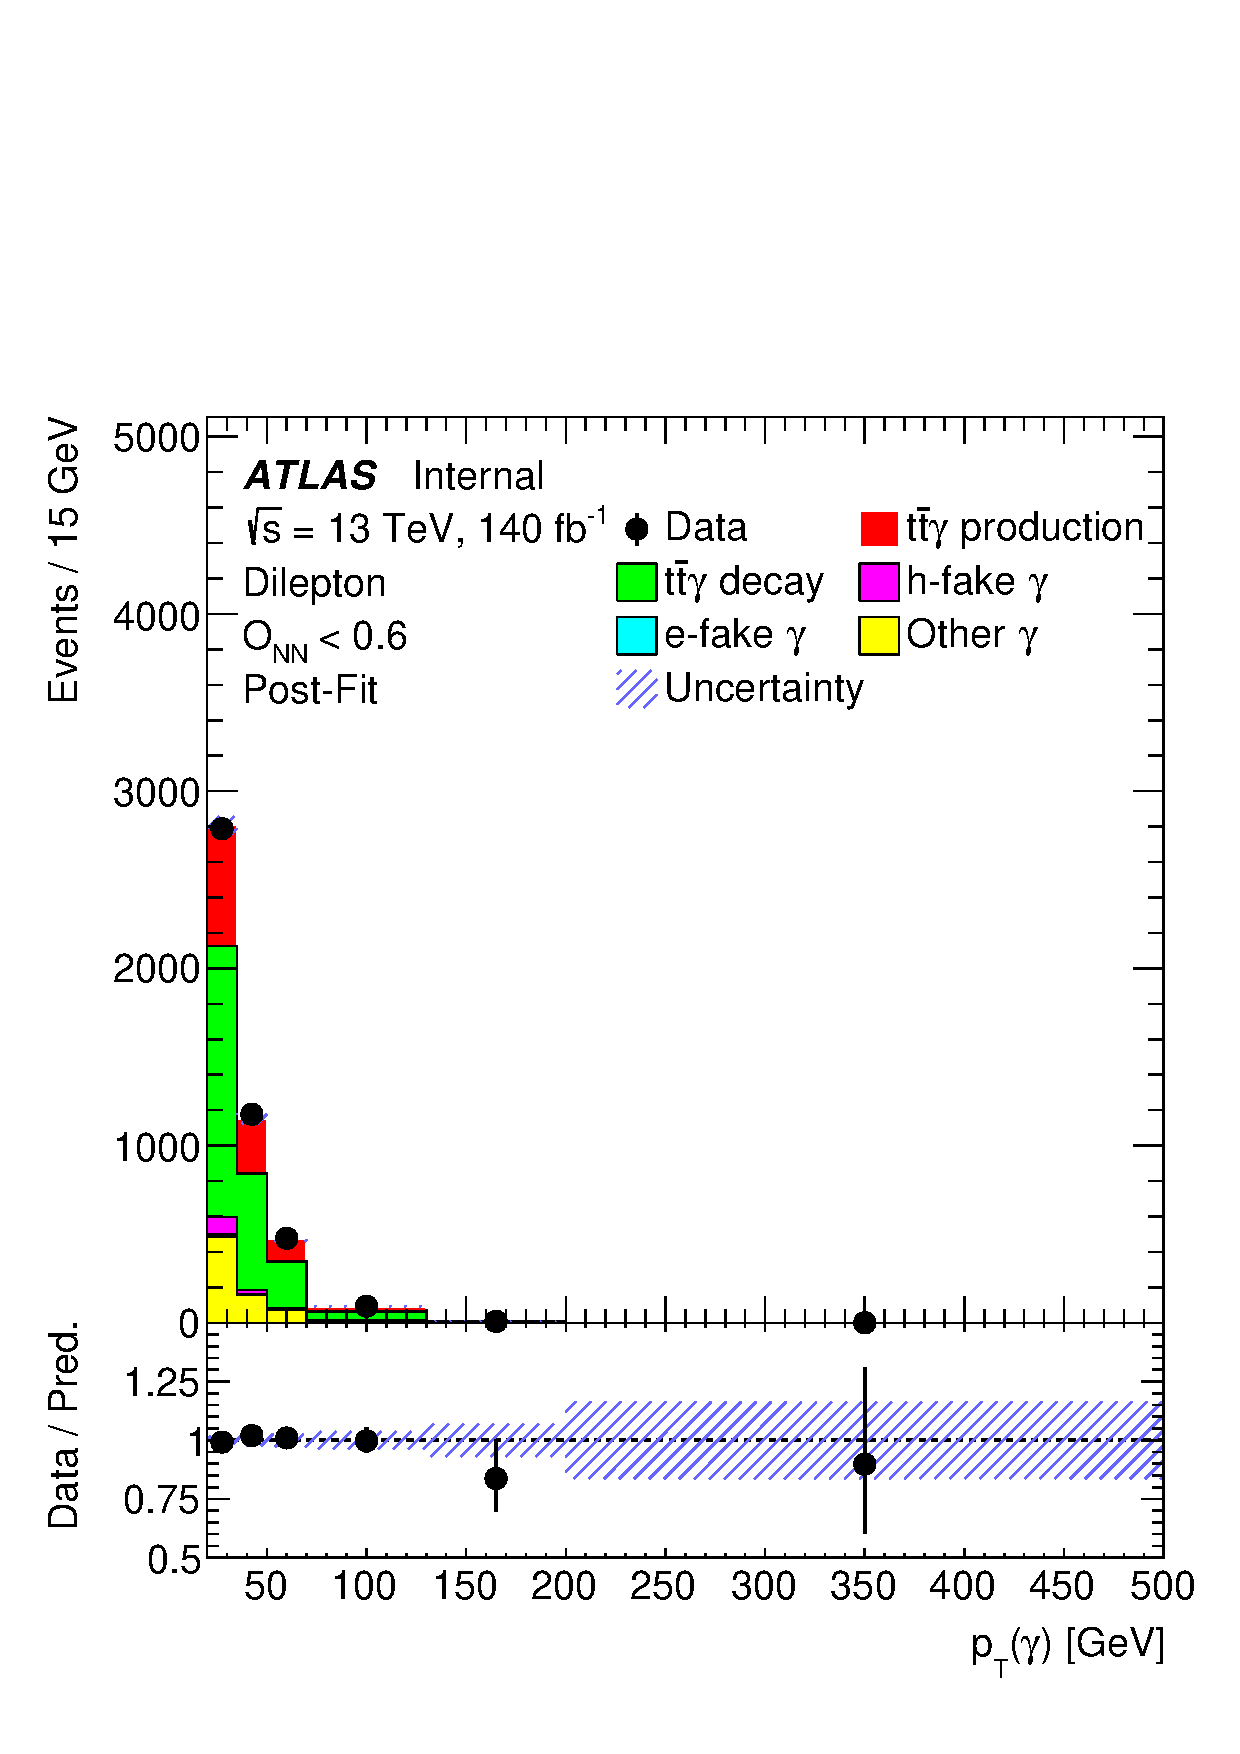
\includegraphics[width=0.30\textwidth]{figures/diff_xsec/dilep/post_fit/tty2l_pt_all_syst/Plots/SR2_postFit.pdf}}
  \caption{The post-fit distributions of $p_T(\gamma)$ in two regions (based on the cut on the Neural Network output) (a) $O_{NN}>=0.6$ (b) $O_{NN}<0.6$ 
  in dilepton channel.}
  \label{fig:pt_postfit_dilep_realdata}
\end{figure}
\FloatBarrier



%% This is the old version of showing the whole pull plot. Below is the new way of showing the plot splitting in half for better visualization 
\begin{comment}
\begin{figure}[ht]
  \centering
  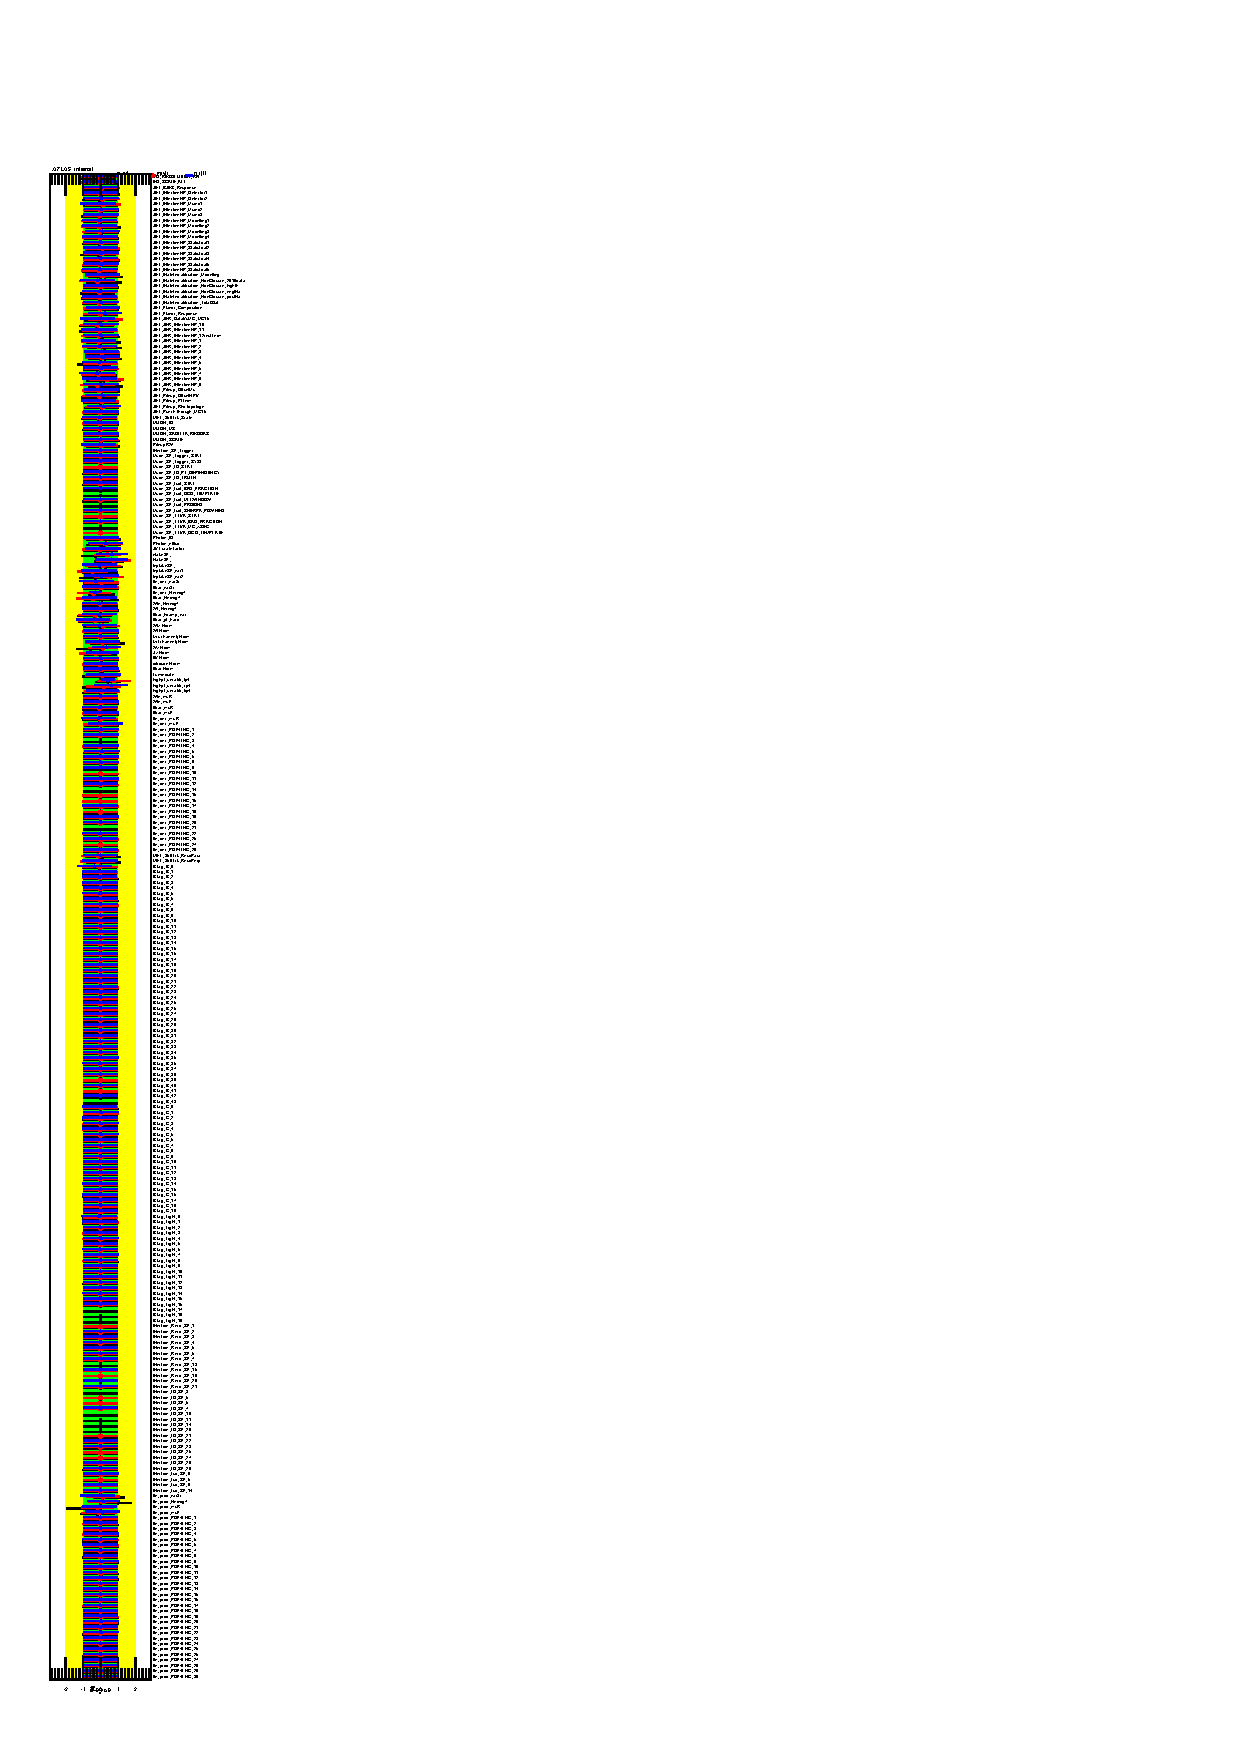
\includegraphics[width=0.20\textwidth]{figures/diff_xsec/ljet_tty_prod_mu_blinded/compare_NP_pulls/compare_NP_dilep_fits_pt_ptj1_eta/NuisPar_comp.pdf}
  \quad \quad
  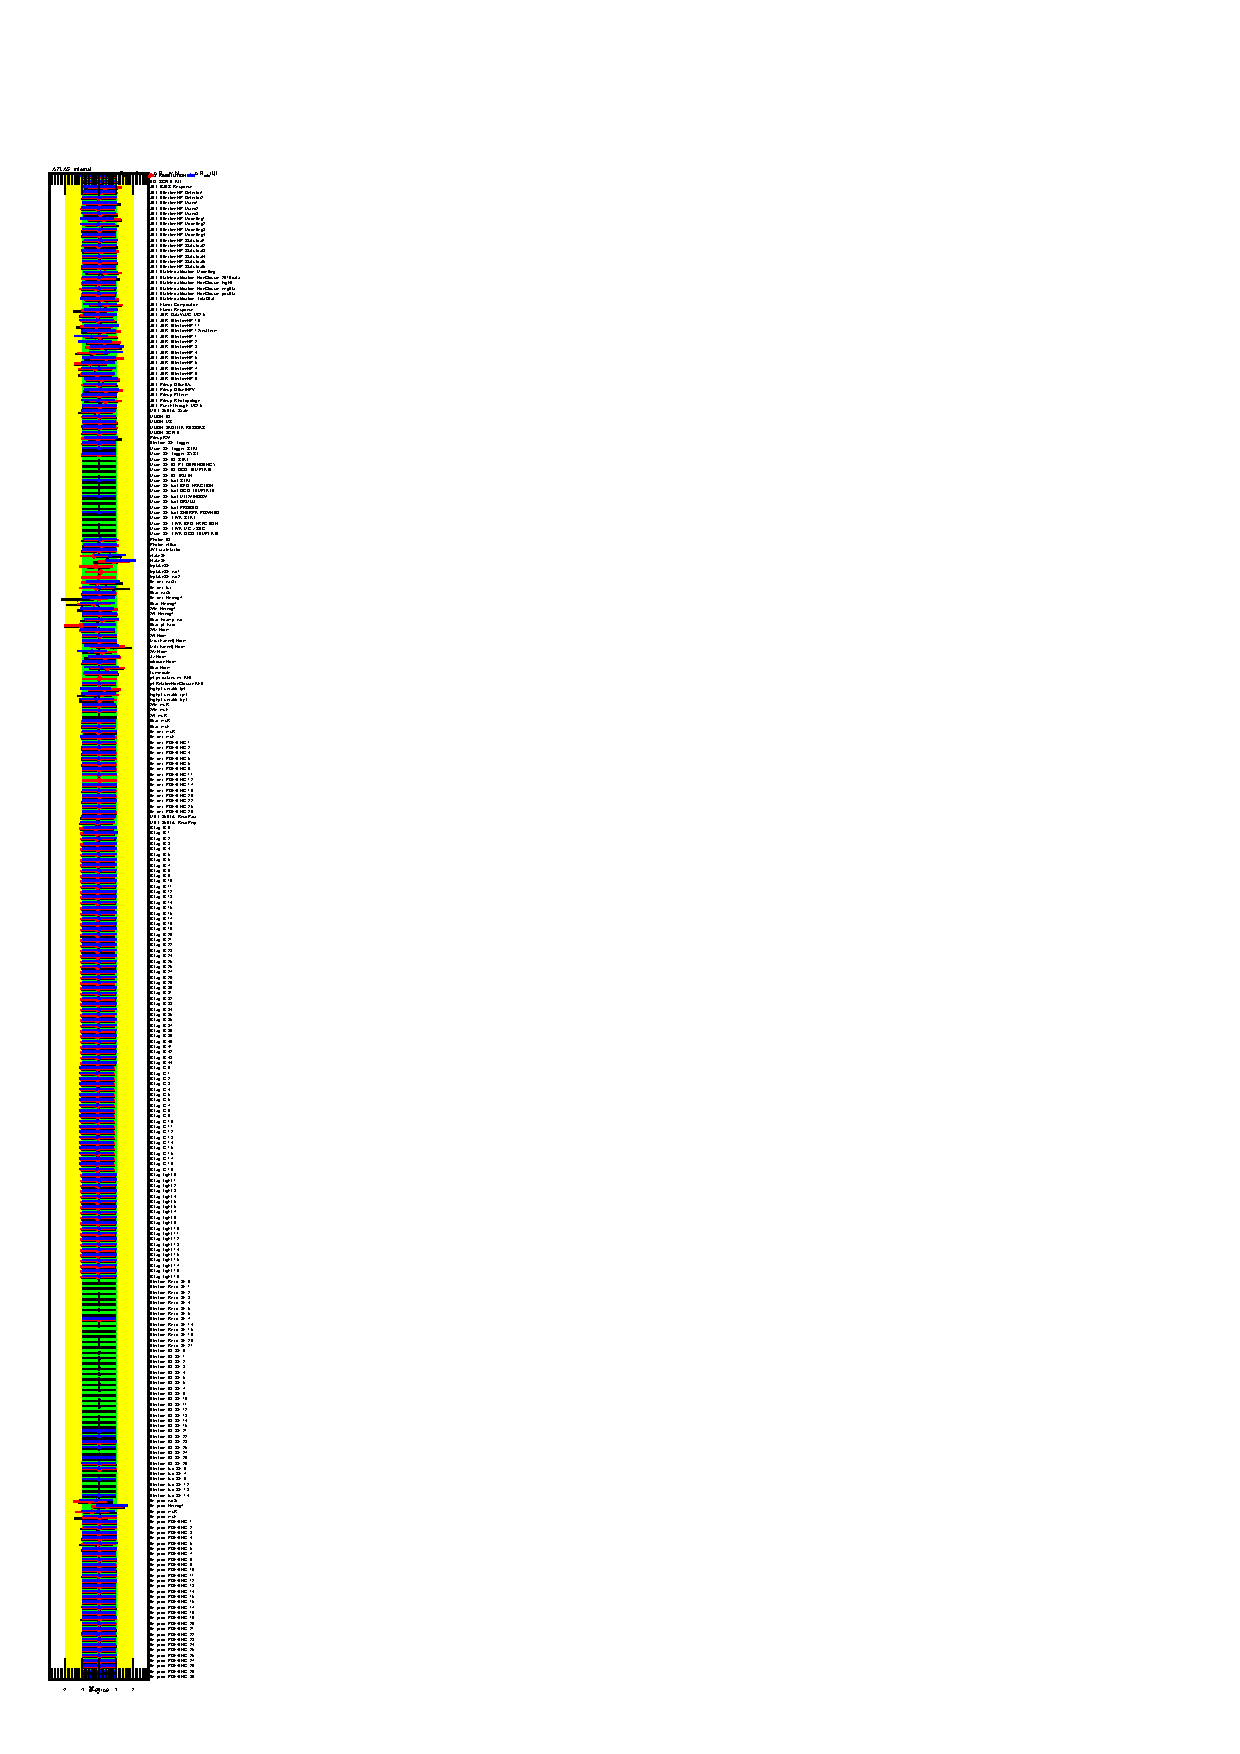
\includegraphics[width=0.20\textwidth]{figures/diff_xsec/ljet_tty_prod_mu_blinded/compare_NP_pulls/compare_NP_dilep_fits_drphb_drlj_dr/NuisPar_comp.pdf}
  \caption{Pull plots obtained from the fit to the data for the l+jet channel, for the \tty (prod.) measurement 
  with the \tty (decay) parameter left as a free variable.}
  \label{fig:pull_plot_pt_tty_dec_free_ljet_mu_blinded}
\end{figure}
\FloatBarrier
\end{comment}



\begin{figure}[ht]
  \centering
  \subfloat[Part 1]{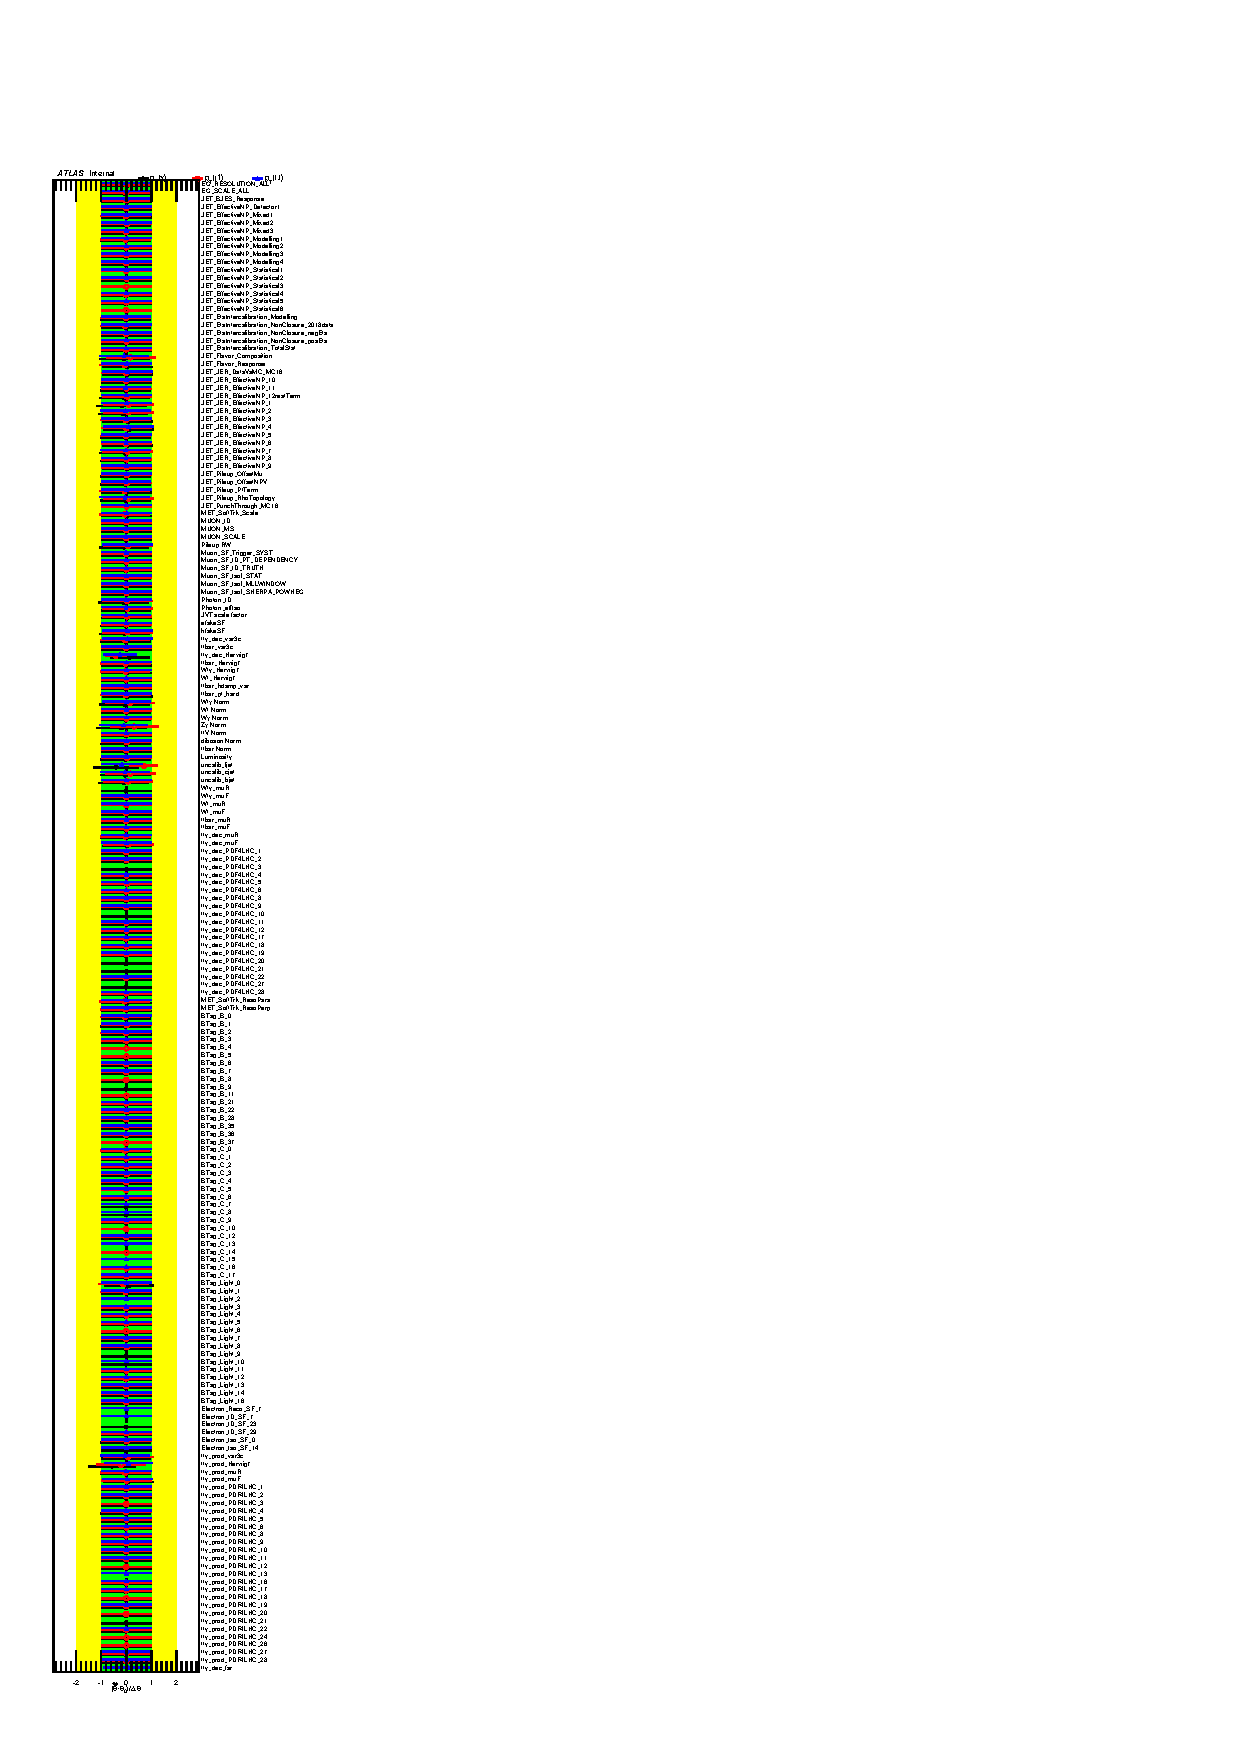
\includegraphics[width=0.40\textwidth, viewport=0 375 150 750, clip]{figures/diff_xsec/dilep_tty_prod_mu_blinded/compare_NP_pulls/compare_NP_dilep_fits_pt_ptj1_ptll/NuisPar_comp.pdf}}
  \quad
  \subfloat[Part 2]{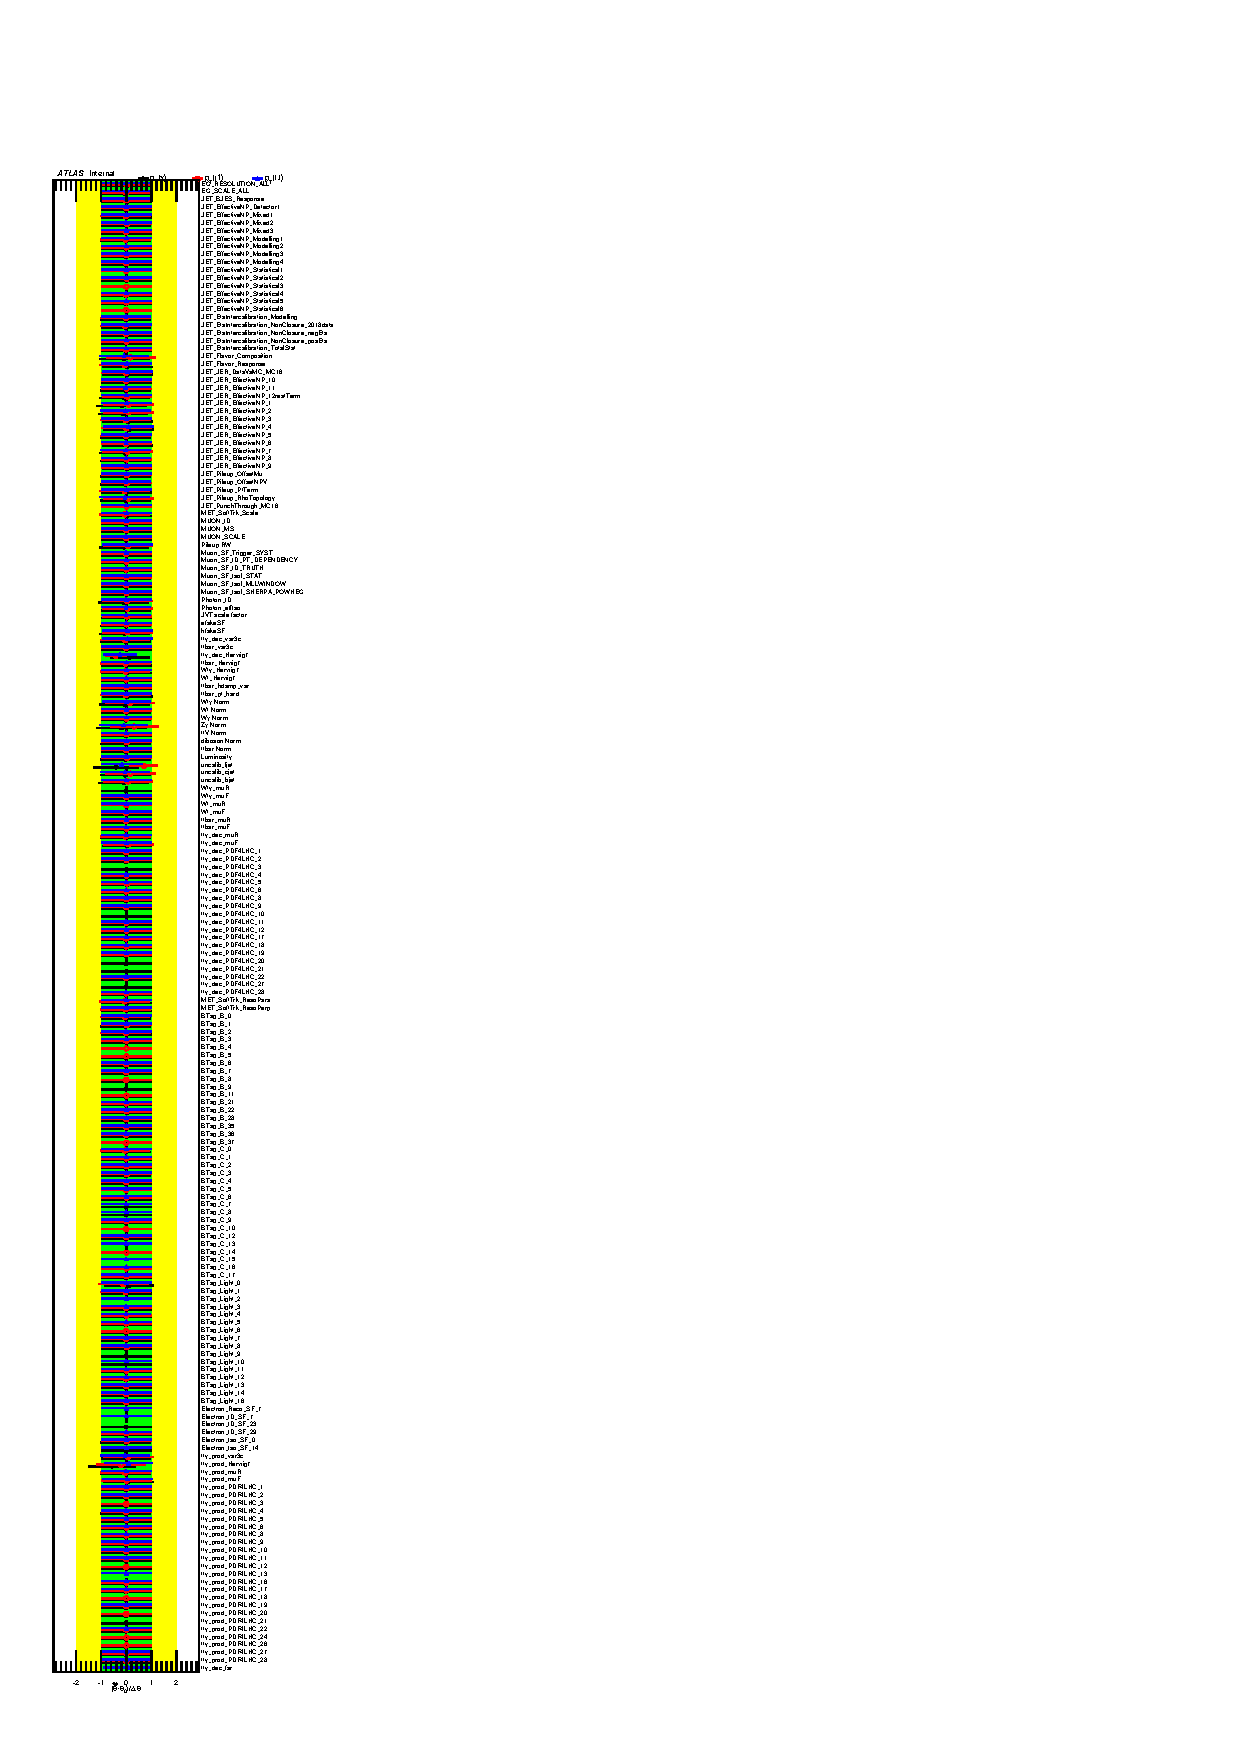
\includegraphics[width=0.40\textwidth, viewport=0 0 150 375, clip]{figures/diff_xsec/dilep_tty_prod_mu_blinded/compare_NP_pulls/compare_NP_dilep_fits_pt_ptj1_ptll/NuisPar_comp.pdf}}
  %\vspace{0.5cm}
  \caption{Pull plots obtained from the fit to the data for the l+jet channel, for the \tty (prod.) measurement 
  with the \tty (decay) parameter left as a free variable.}
  \label{fig:pull_plot_pt_tty_dec_free_ljet_mu_blinded}
\end{figure}

\begin{figure}[ht]
  \centering
  \subfloat[Part 3]{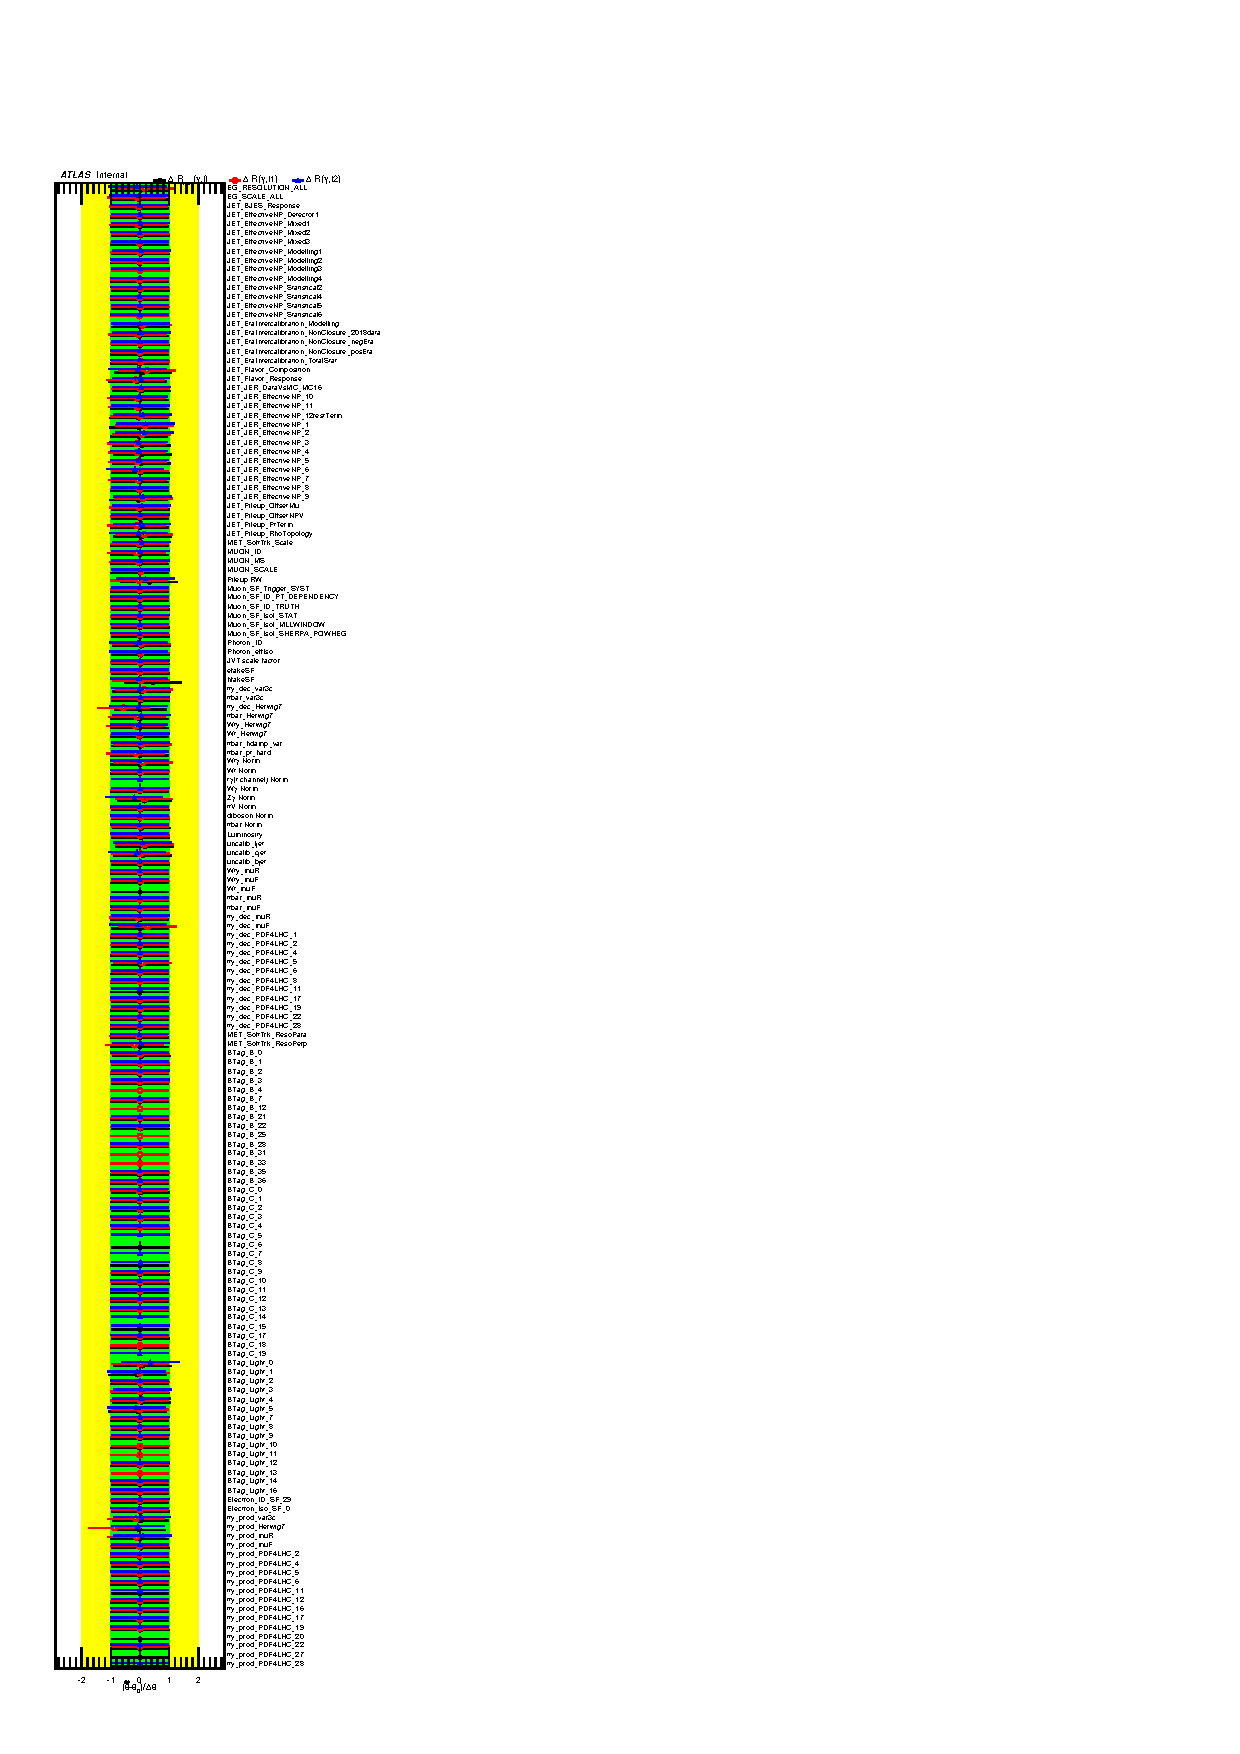
\includegraphics[width=0.40\textwidth, viewport=0 375 150 750, clip]{figures/diff_xsec/dilep_tty_prod_mu_blinded/compare_NP_pulls/compare_NP_dilep_fits_dr_dr1_dr2/NuisPar_comp.pdf}}
  \quad
  \subfloat[Part 4]{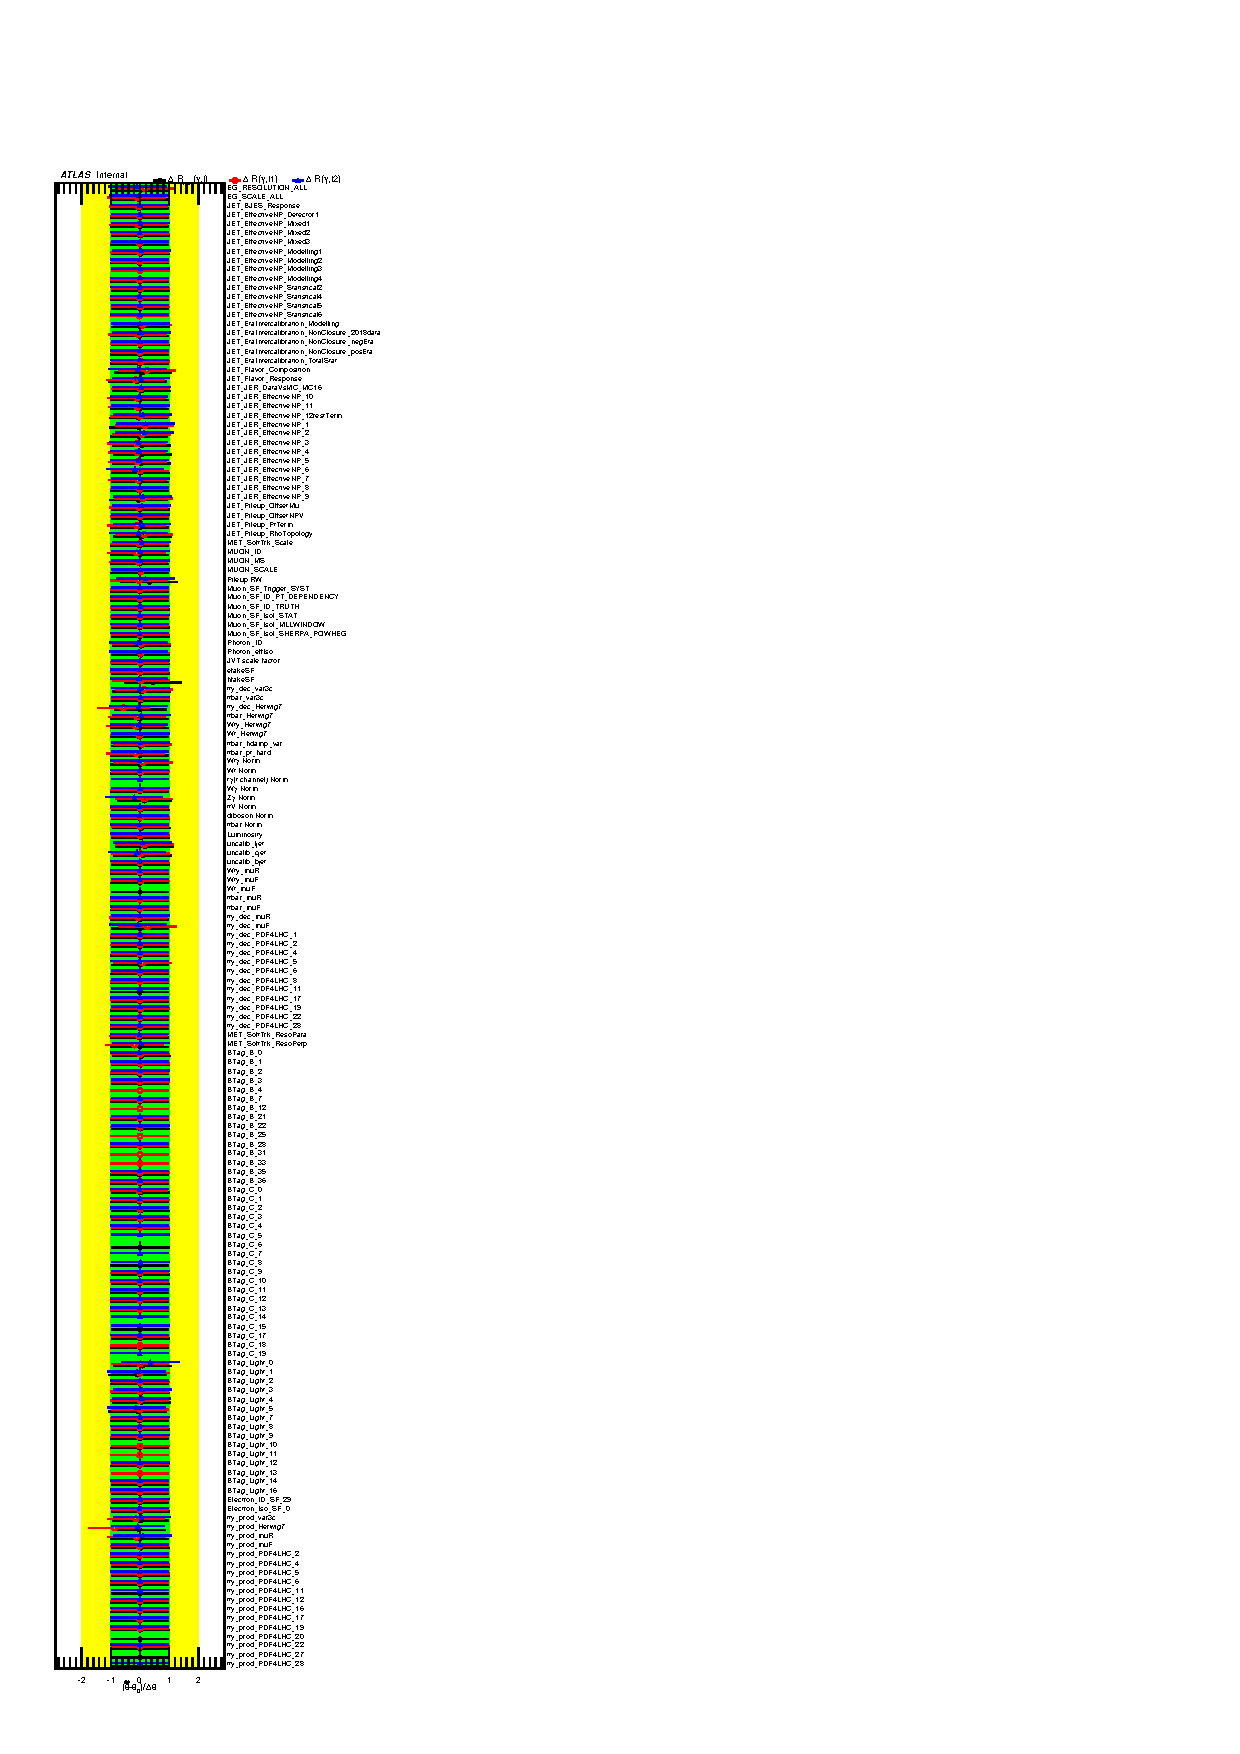
\includegraphics[width=0.40\textwidth, viewport=0 0 150 375, clip]{figures/diff_xsec/dilep_tty_prod_mu_blinded/compare_NP_pulls/compare_NP_dilep_fits_dr_dr1_dr2/NuisPar_comp.pdf}}
  \caption{Pull plots obtained from the fit to the data for the l+jet channel, for the \tty (prod.) measurement 
  with the \tty (decay) parameter left as a free variable.}
  \label{fig:pull_plot_pt_tty_dec_free_ljet_mu_blinded}

\end{figure}


\begin{figure}[ht]
  \centering
  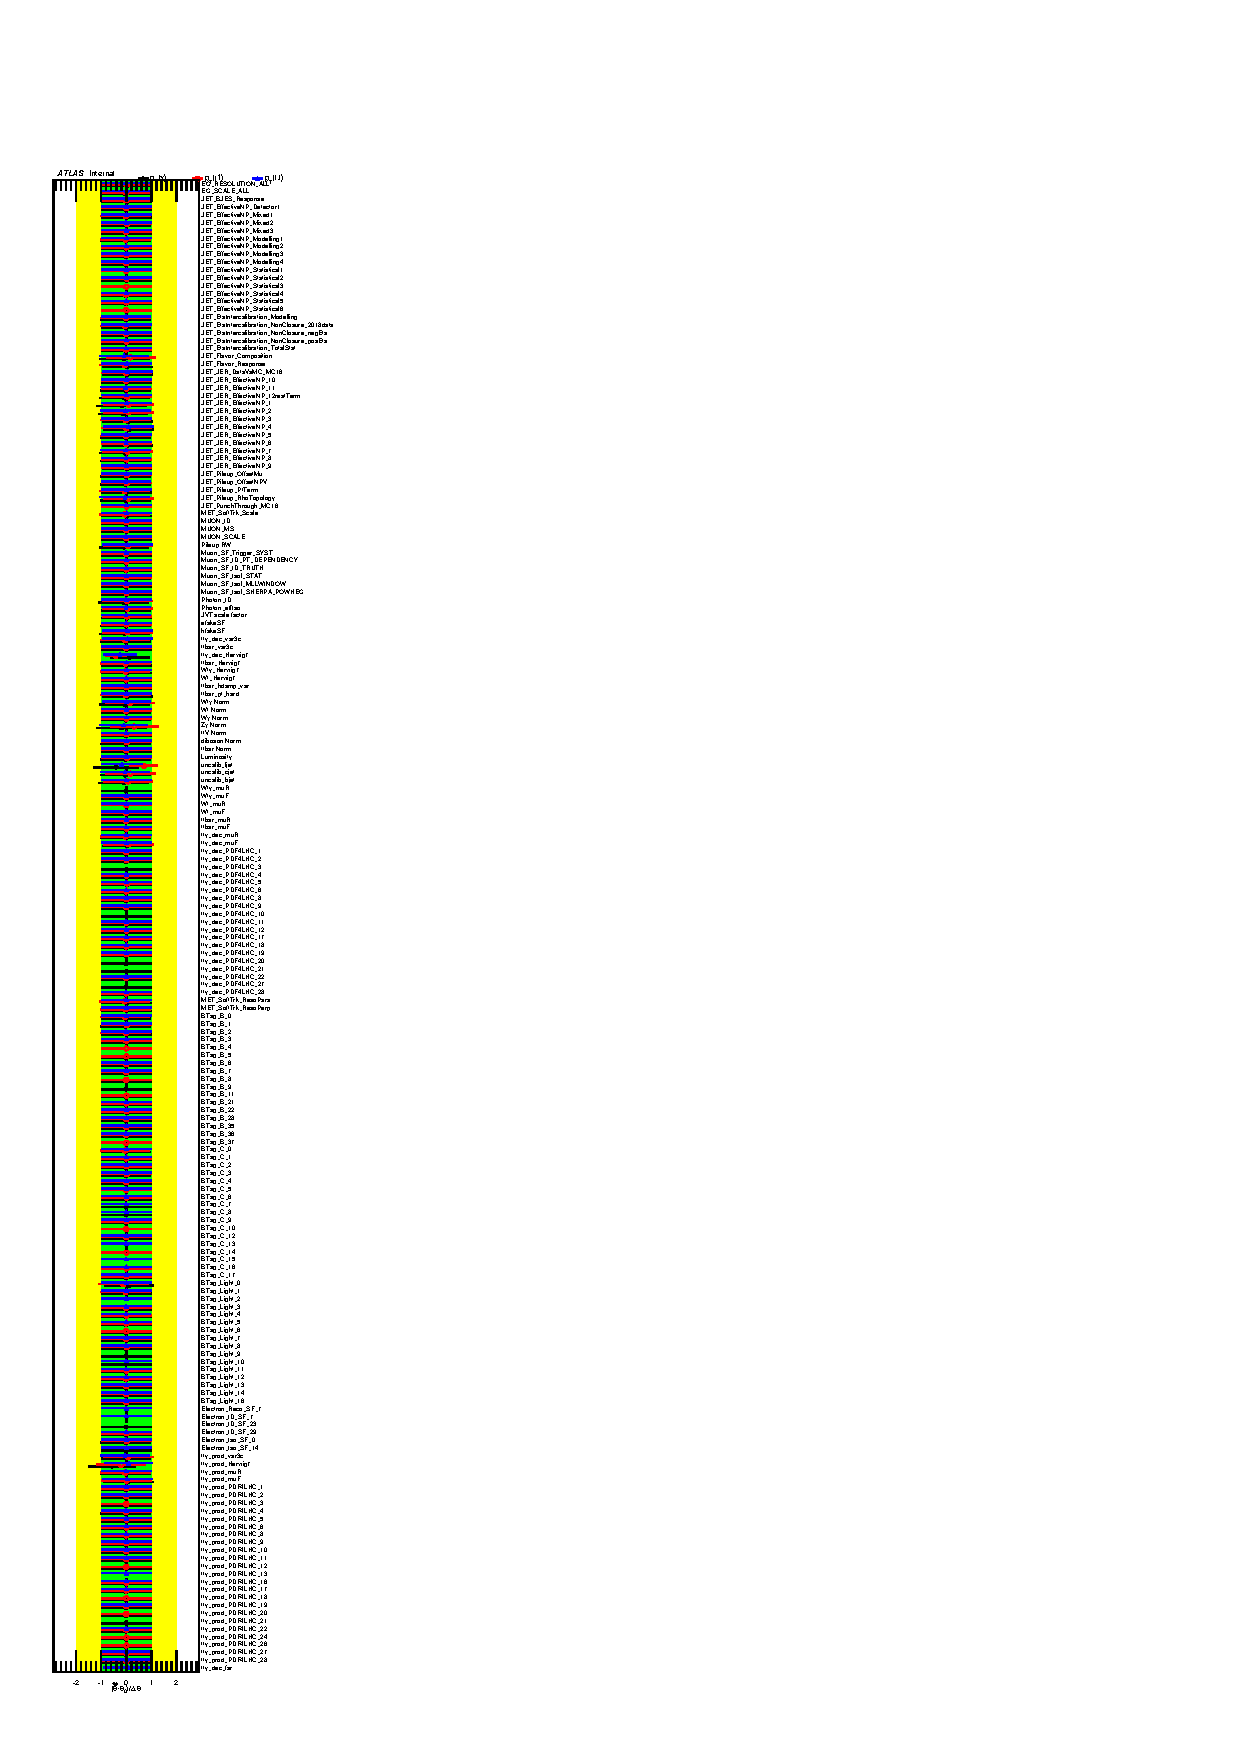
\includegraphics[width=0.35\textwidth]{figures/diff_xsec/dilep_tty_prod_mu_blinded/compare_NP_pulls/compare_NP_dilep_fits_pt_ptj1_ptll/NuisPar_comp.pdf}
  \quad \quad 
  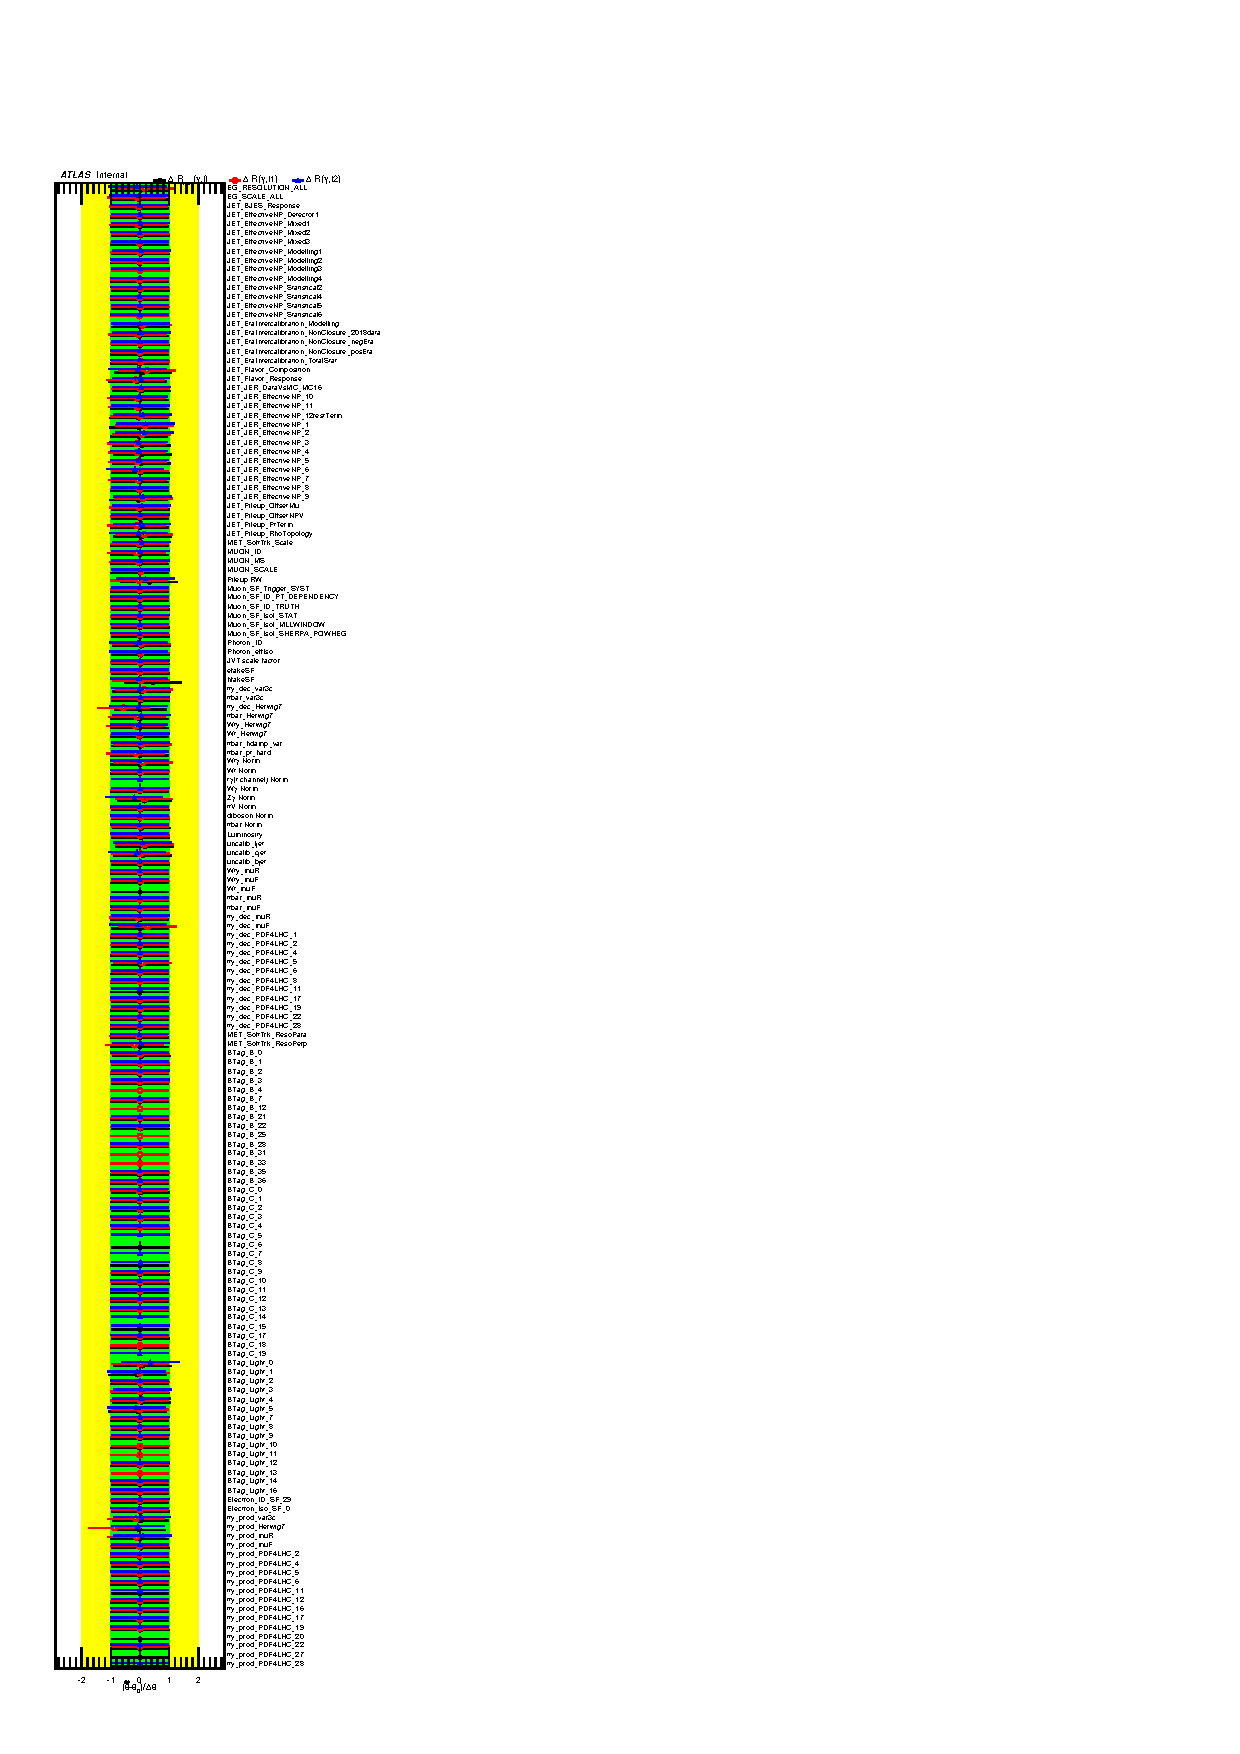
\includegraphics[width=0.35\textwidth]{figures/diff_xsec/dilep_tty_prod_mu_blinded/compare_NP_pulls/compare_NP_dilep_fits_dr_dr1_dr2/NuisPar_comp.pdf}
  %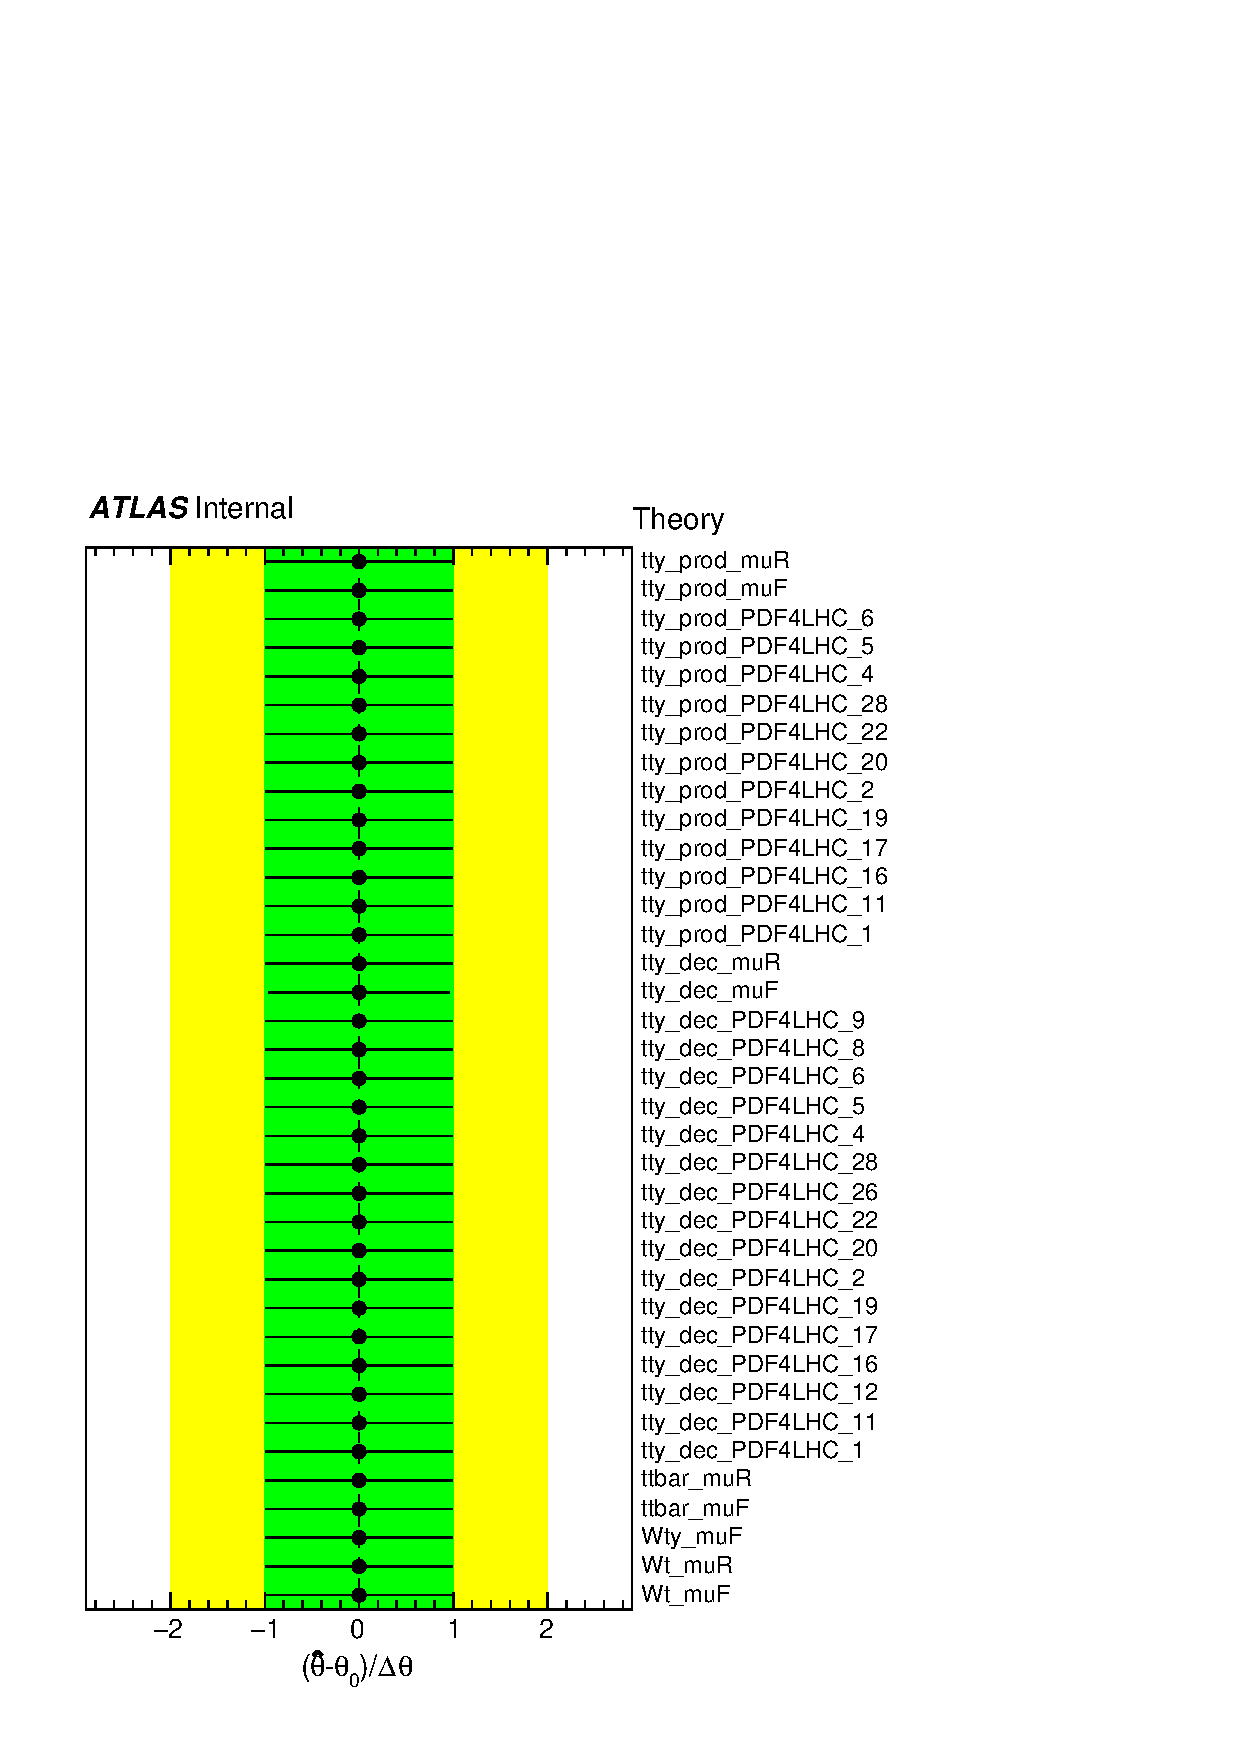
\includegraphics[width=0.32\textwidth]{figures/diff_xsec/dilep/Unfolded_data_tty_dec_free_mu_blinded/compare_NP_dilep_fits_pt_ptj1_ptll/NuisPar_Theory.pdf}
  \caption{Pull plots obtained from the fit to the data for the dilepton channel, for the \tty (prod.) measurement
  with the \tty (decay) parameter left as a free variable.}
  \label{fig:pull_plot_pt_tty_dec_free_dilep_mu_blinded_1}
\end{figure}
\FloatBarrier

\begin{figure}[ht]
  \centering
  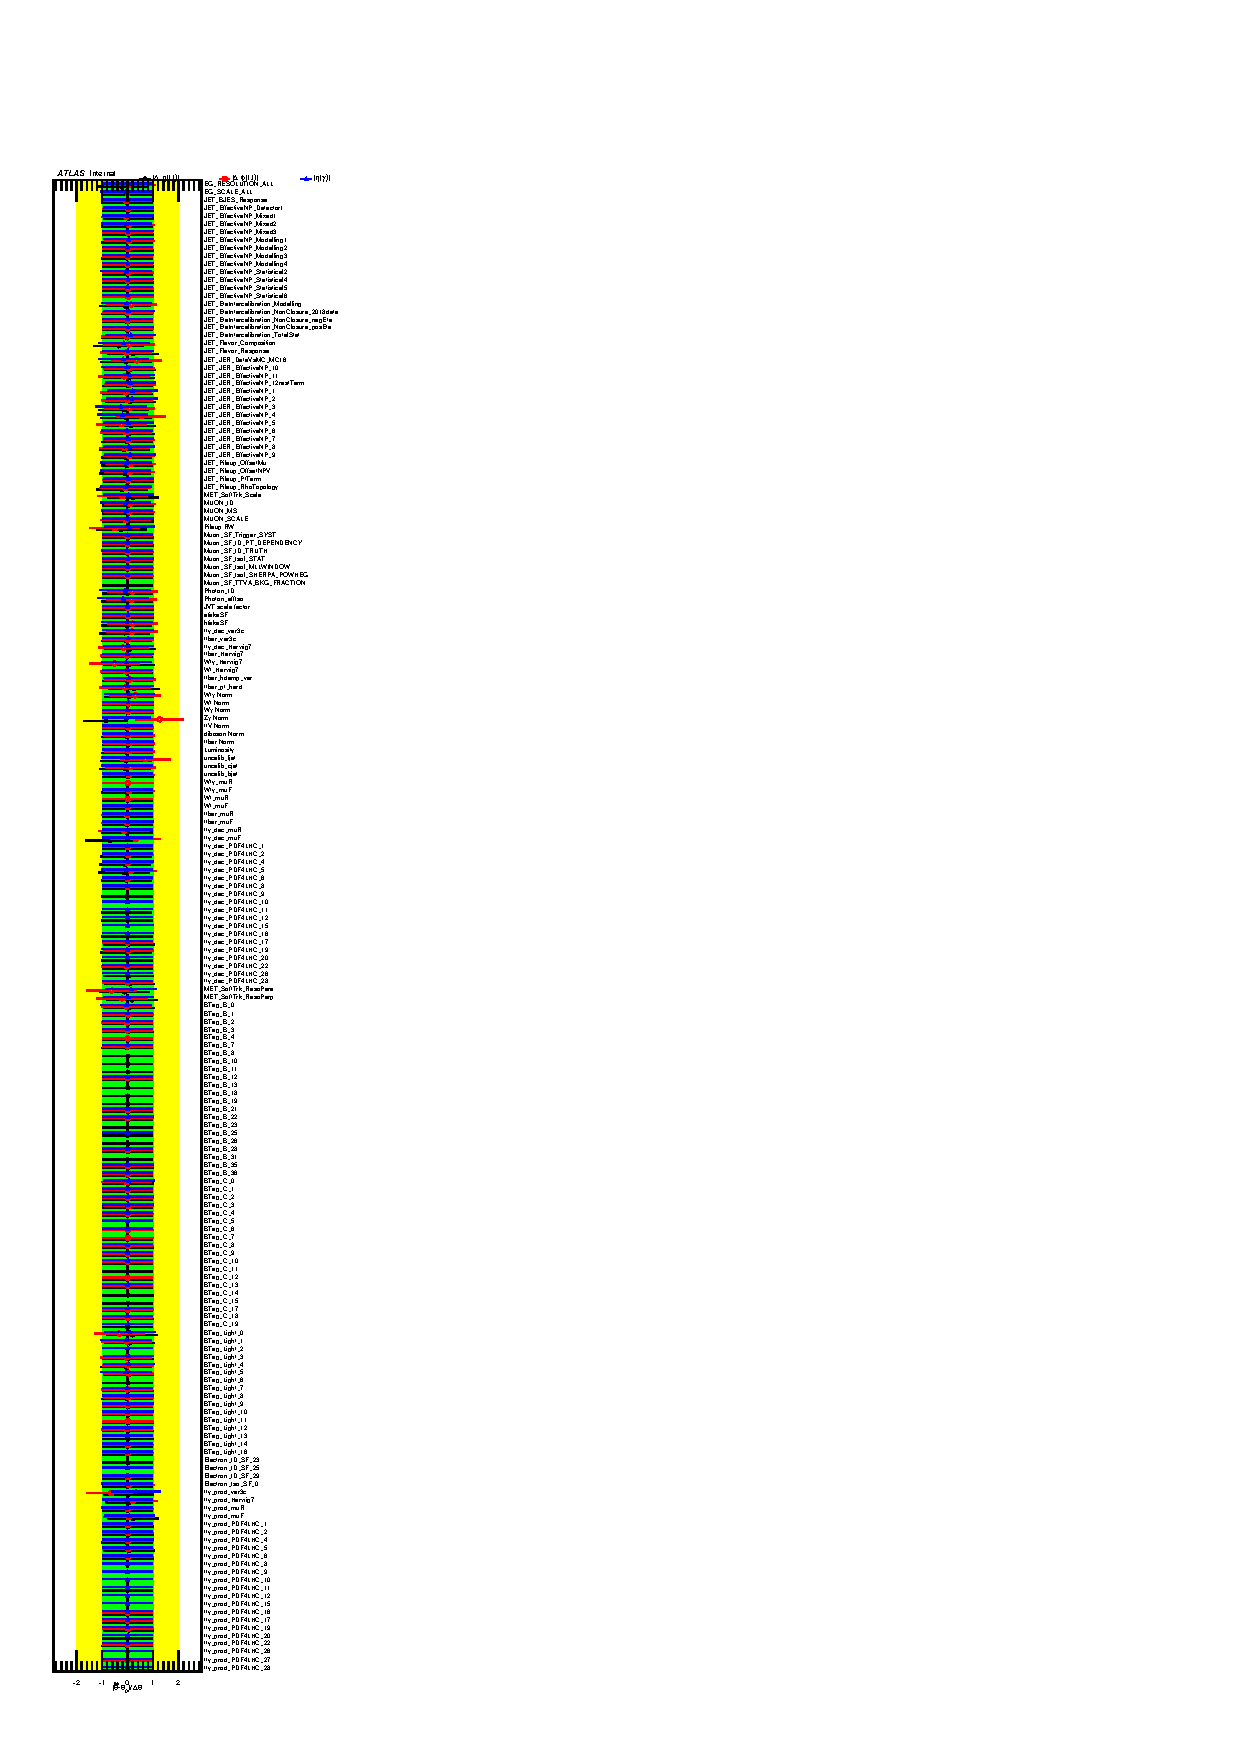
\includegraphics[width=0.35\textwidth]{figures/diff_xsec/dilep_tty_prod_mu_blinded/compare_NP_pulls/compare_NP_dilep_fits_detall_dphill_eta/NuisPar_comp.pdf}
  \quad \quad
  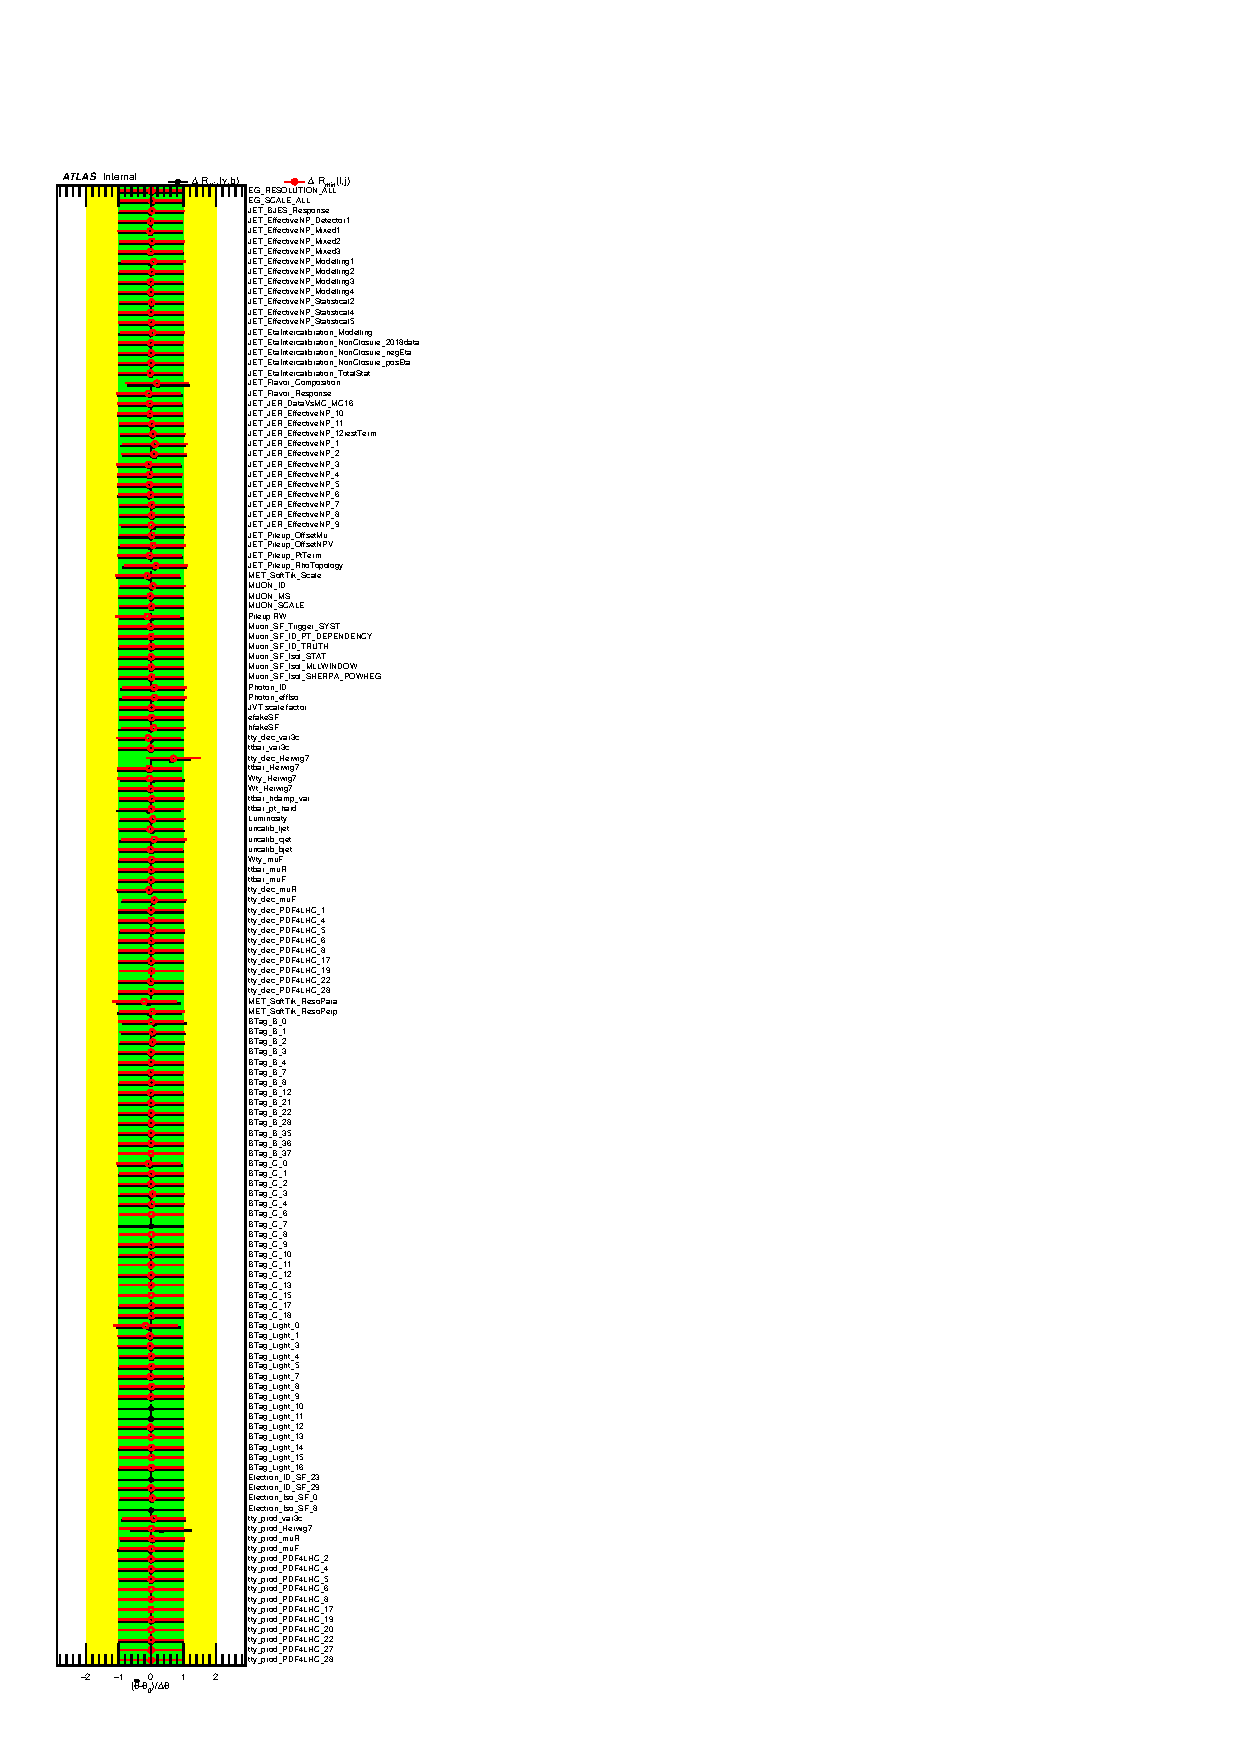
\includegraphics[width=0.35\textwidth]{figures/diff_xsec/dilep_tty_prod_mu_blinded/compare_NP_pulls/compare_NP_dilep_fits_drphb_drlj/NuisPar_comp.pdf}
  \caption{Pull plots obtained from the fit to the data for the dilepton channel, for the \tty (prod.) measurement
  with the \tty (decay) parameter left as a free variable.}
  \label{fig:pull_plot_pt_tty_dec_free_dilep_mu_blinded_2}
\end{figure}
\FloatBarrier



\begin{figure}[ht]
  \centering
  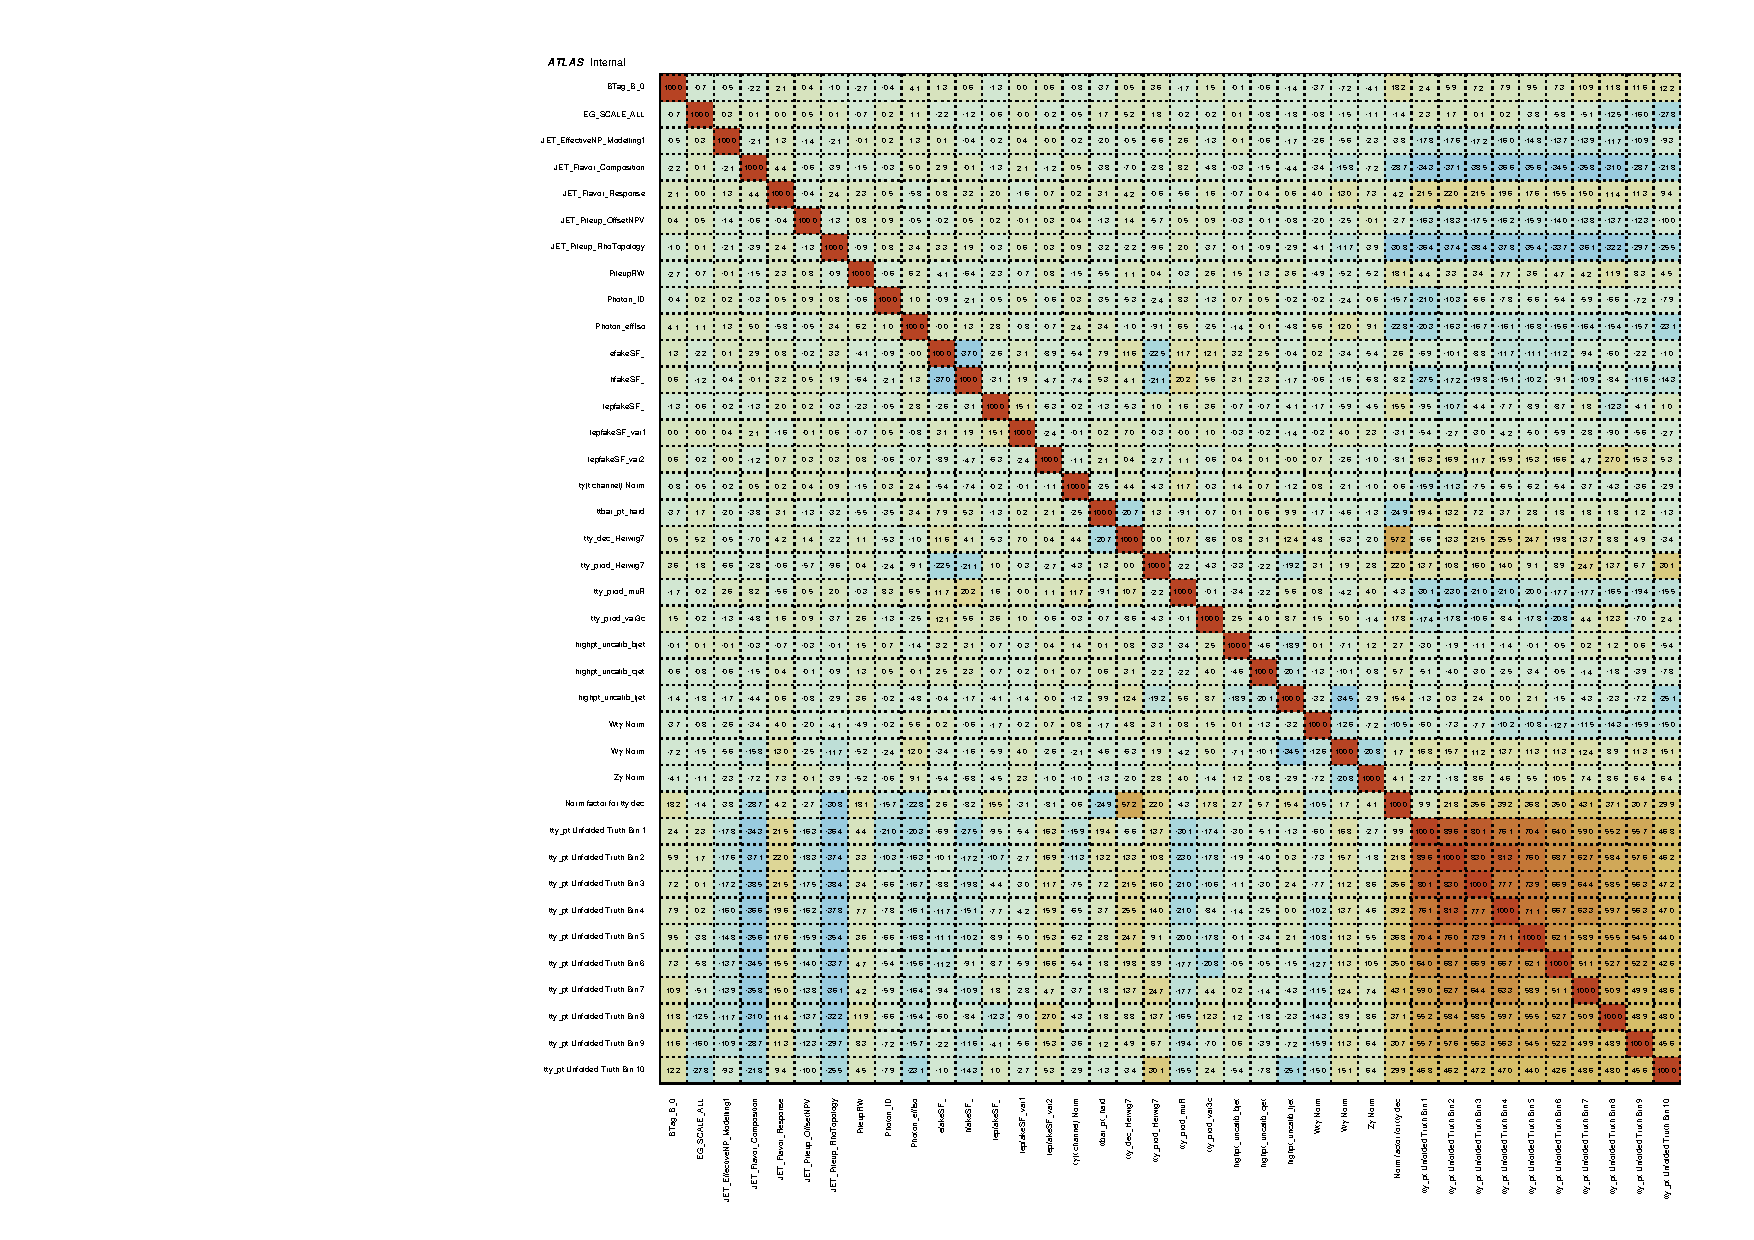
\includegraphics[width=0.8\textwidth]{figures/diff_xsec/ljet_tty_prod_mu_blinded/correlations/tty1l_pt_all_syst/CorrMatrix.pdf}
  \caption{The correlation between the NPs and POIs for the measurement of 
  the $p_T(\gamma)$ distribution in single lepton channel for the \tty(prod) measurement.}
  \label{fig:NP-corr_ljet_mu_blinded}
\end{figure}
\FloatBarrier


\begin{figure}[ht]
  \centering
  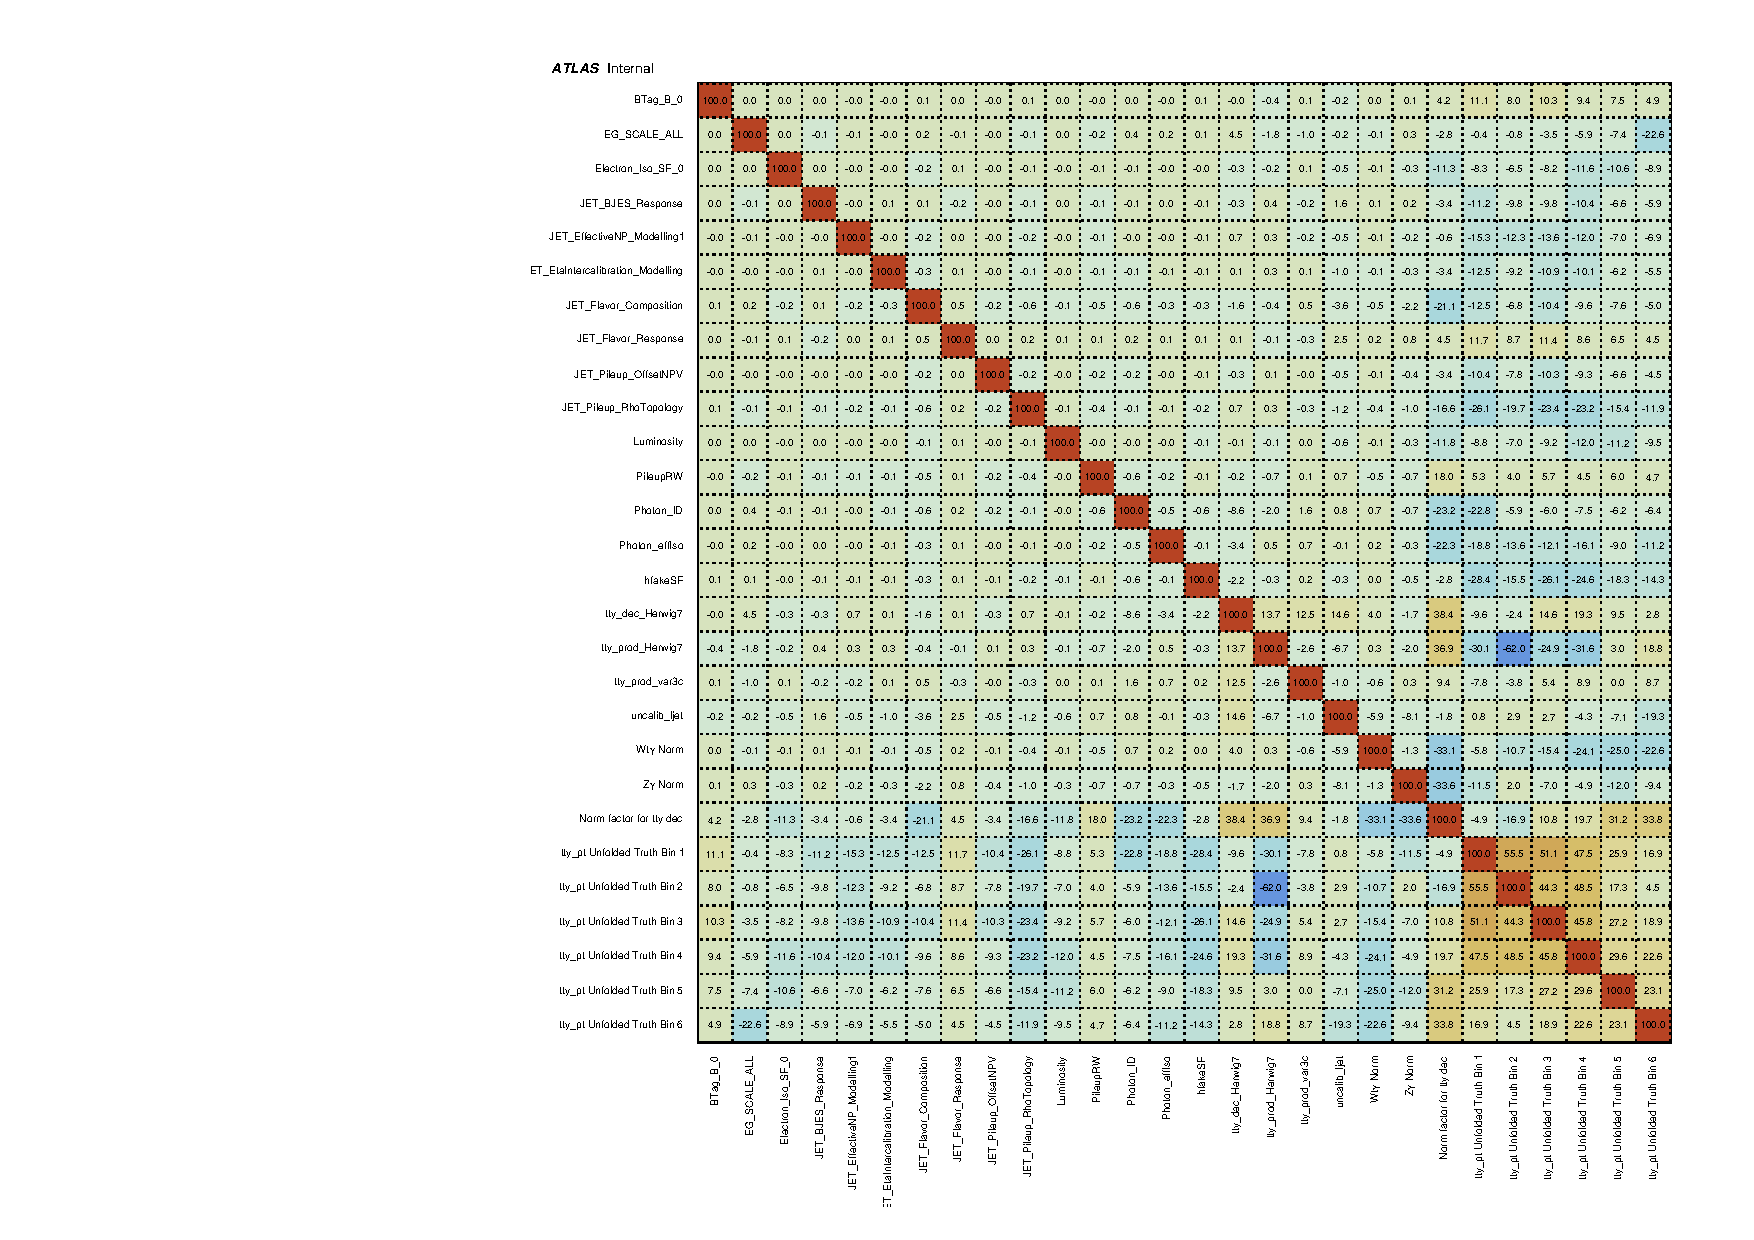
\includegraphics[width=0.8\textwidth]{figures/diff_xsec/dilep_tty_prod_mu_blinded/correlations/tty2l_pt_all_syst/CorrMatrix.pdf}
  \caption{The correlation between the NPs and POIs for the measurement of 
  the $p_T(\gamma)$ distribution in dilepton channel for the \tty (prod.) measurement.}
  \label{fig:NP-corr_dilep_mu_blinded}
\end{figure}
\FloatBarrier

%%%%%%%%%%%% RANKING %%%%%%%%%%%%%%%%%%%

\begin{figure}[ht]
  \centering
  \subfloat[]{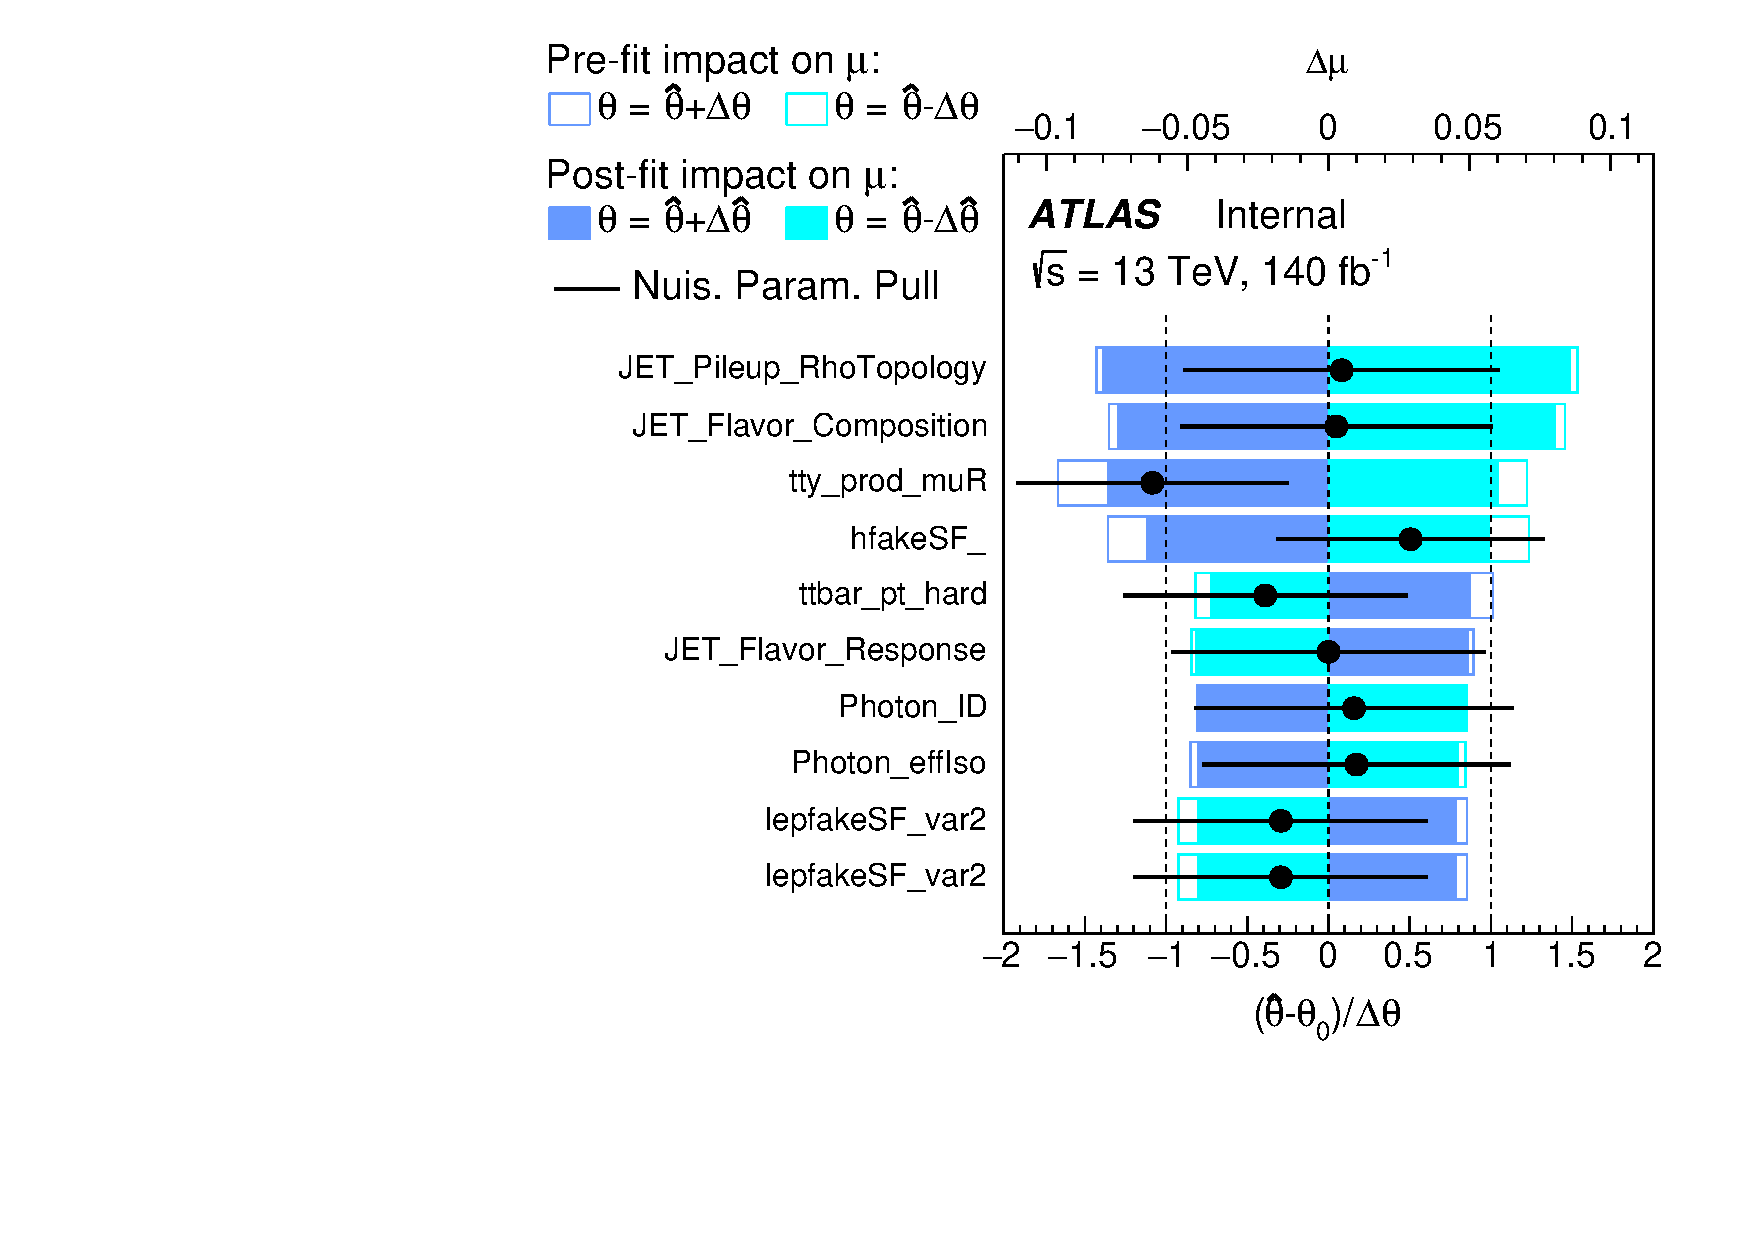
\includegraphics[width=0.2\textwidth]{figures/diff_xsec/ljet_tty_prod_mu_blinded/Ranking/tty1l_pt_all_syst/Ranking_tty_pt_Bin_001_mu.pdf}}
  \quad
  \subfloat[]{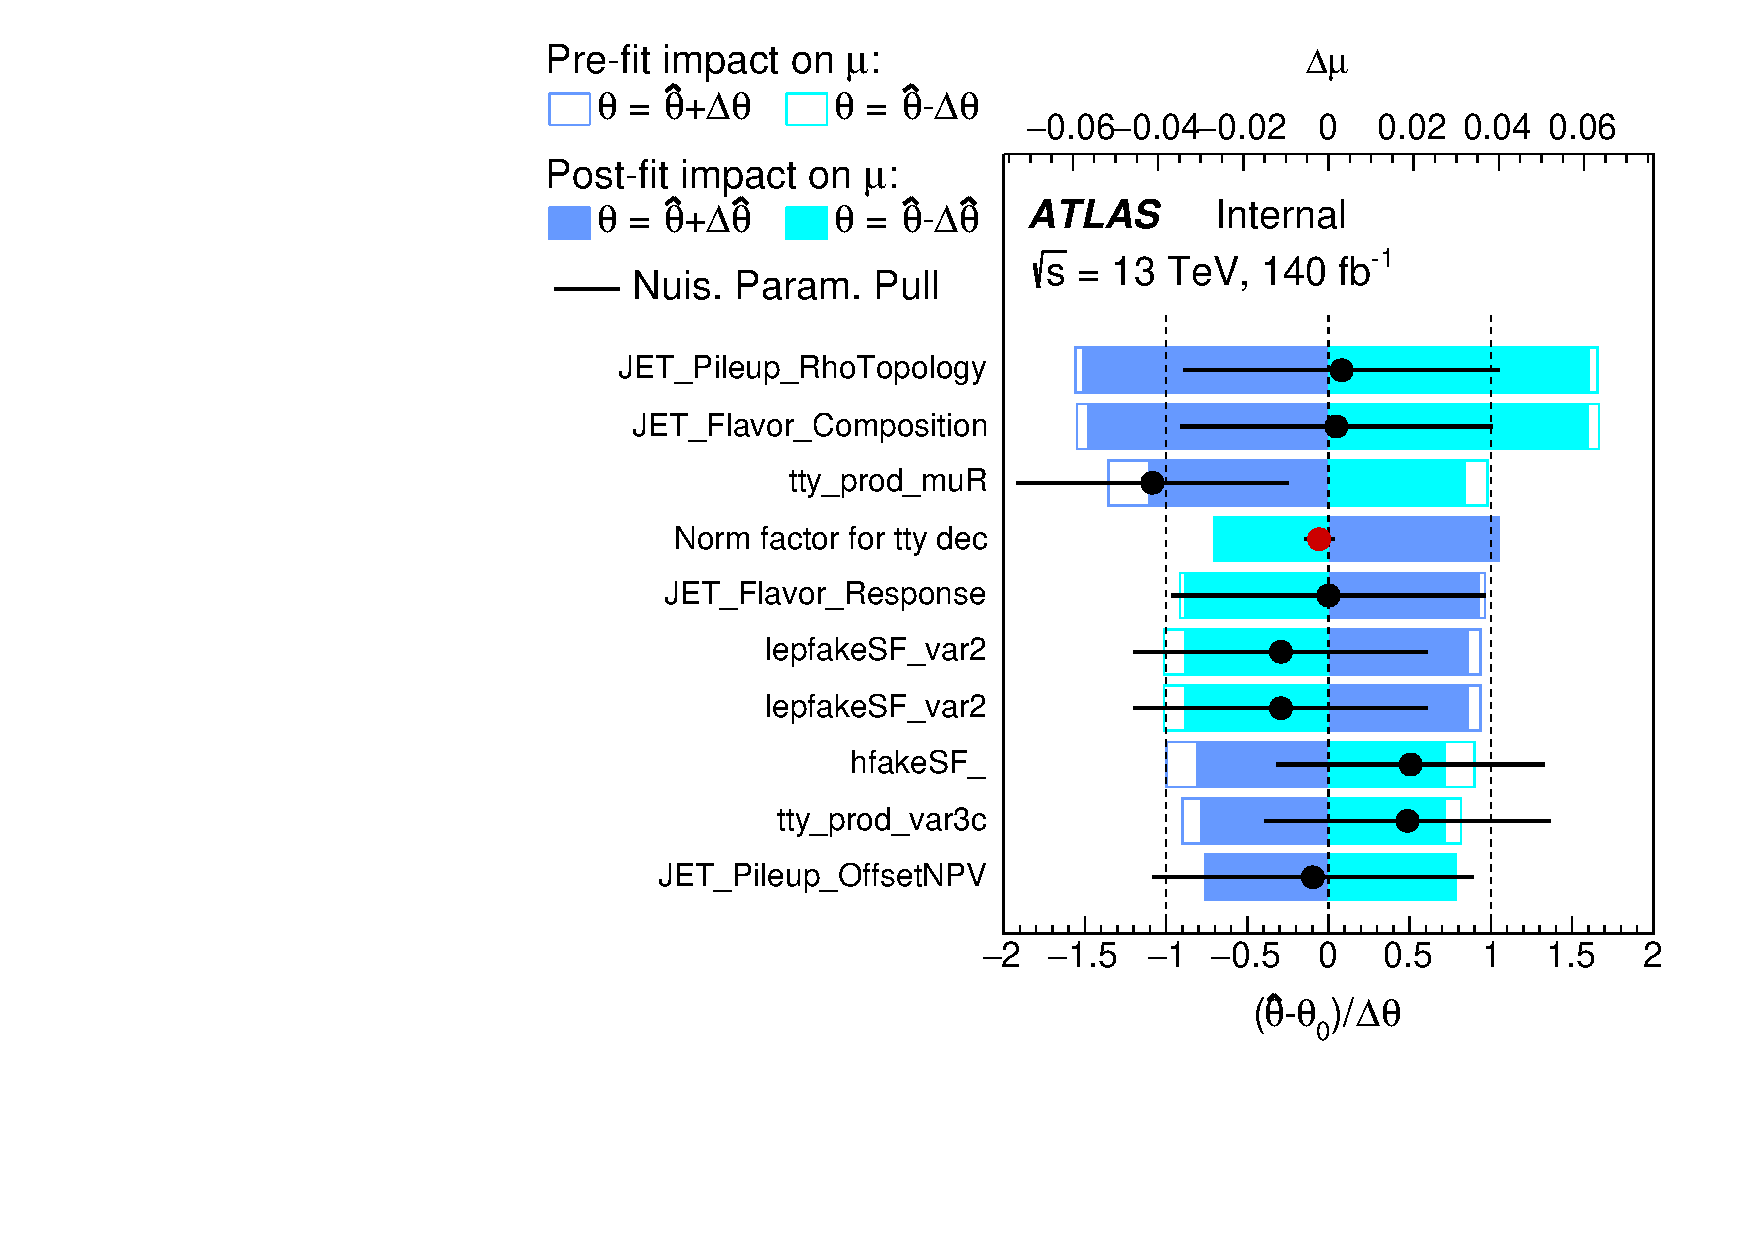
\includegraphics[width=0.2\textwidth]{figures/diff_xsec/ljet_tty_prod_mu_blinded/Ranking/tty1l_pt_all_syst/Ranking_tty_pt_Bin_002_mu.pdf}}
  \quad
  \subfloat[]{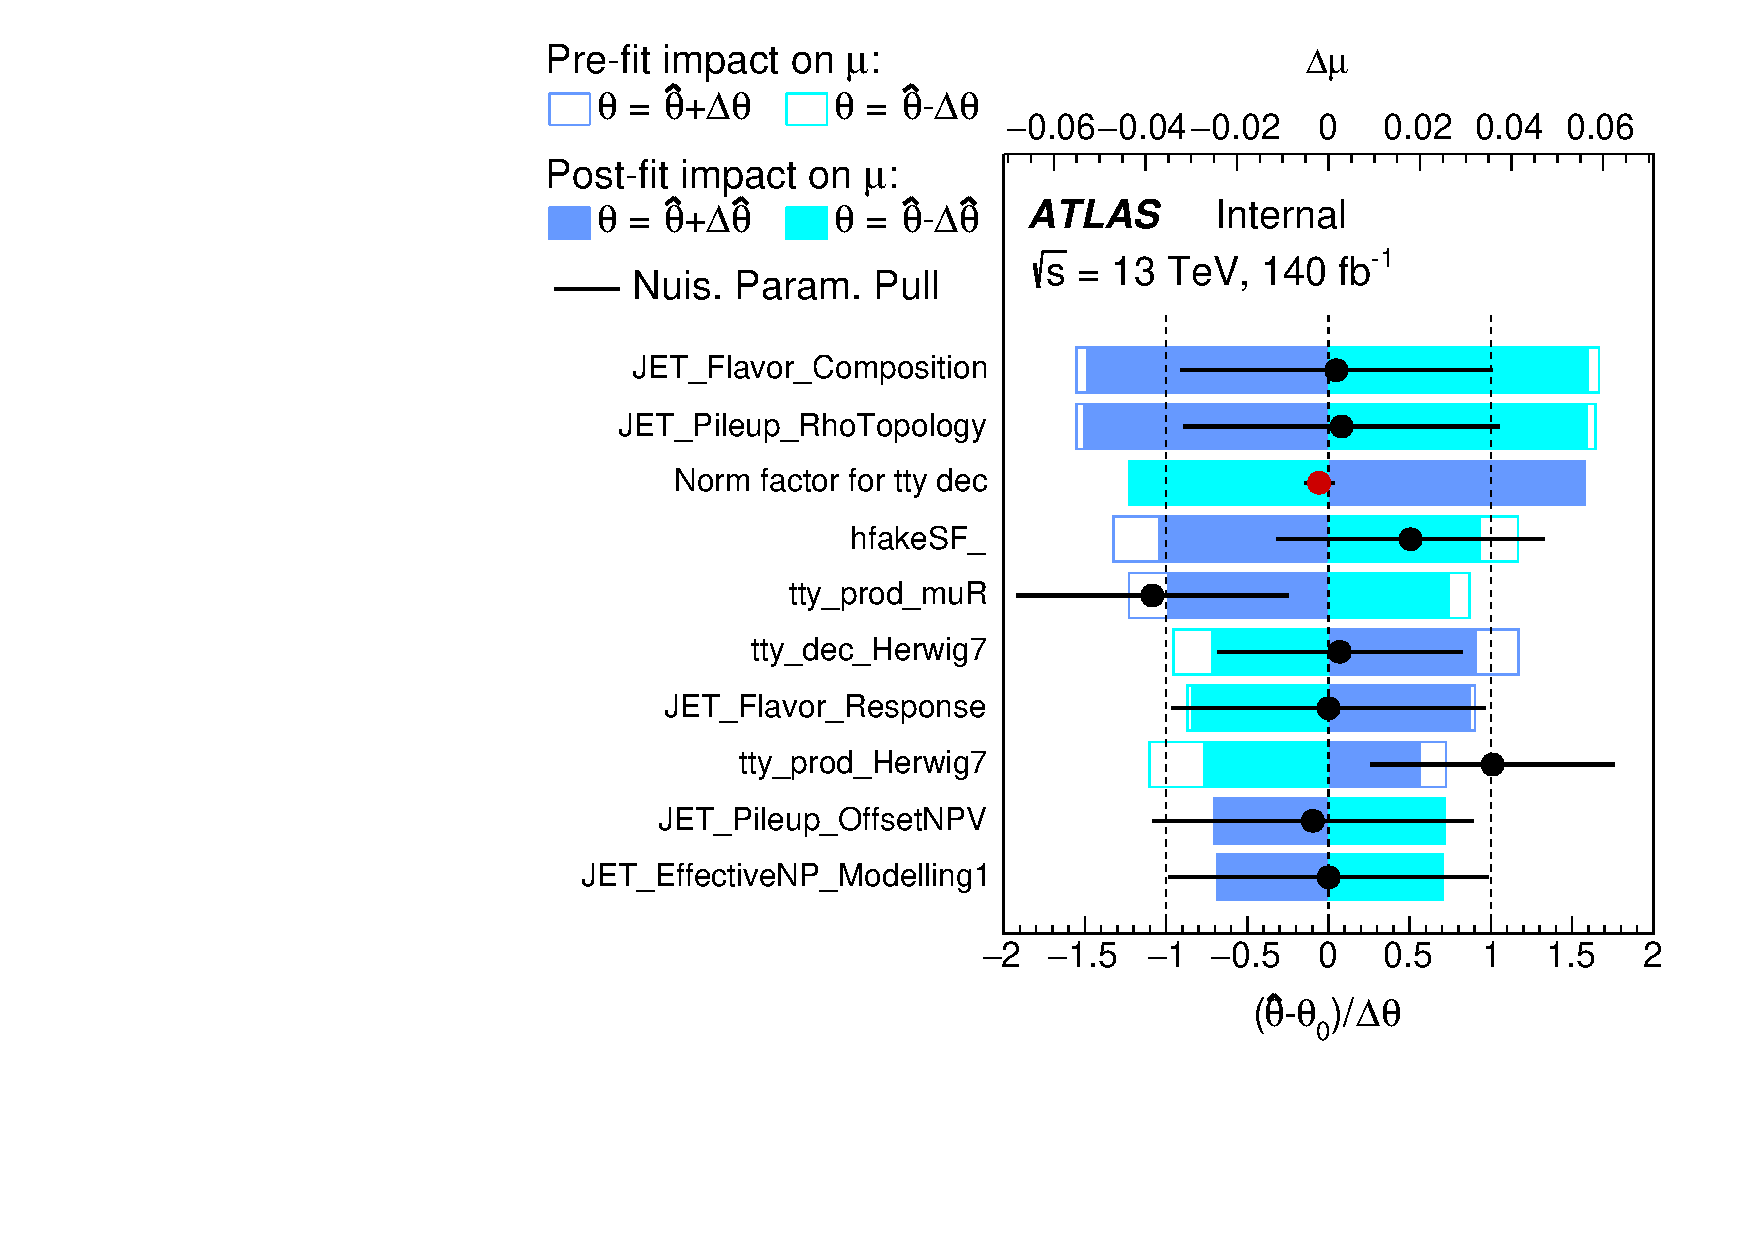
\includegraphics[width=0.2\textwidth]{figures/diff_xsec/ljet_tty_prod_mu_blinded/Ranking/tty1l_pt_all_syst/Ranking_tty_pt_Bin_003_mu.pdf}}
  \quad
  \subfloat[]{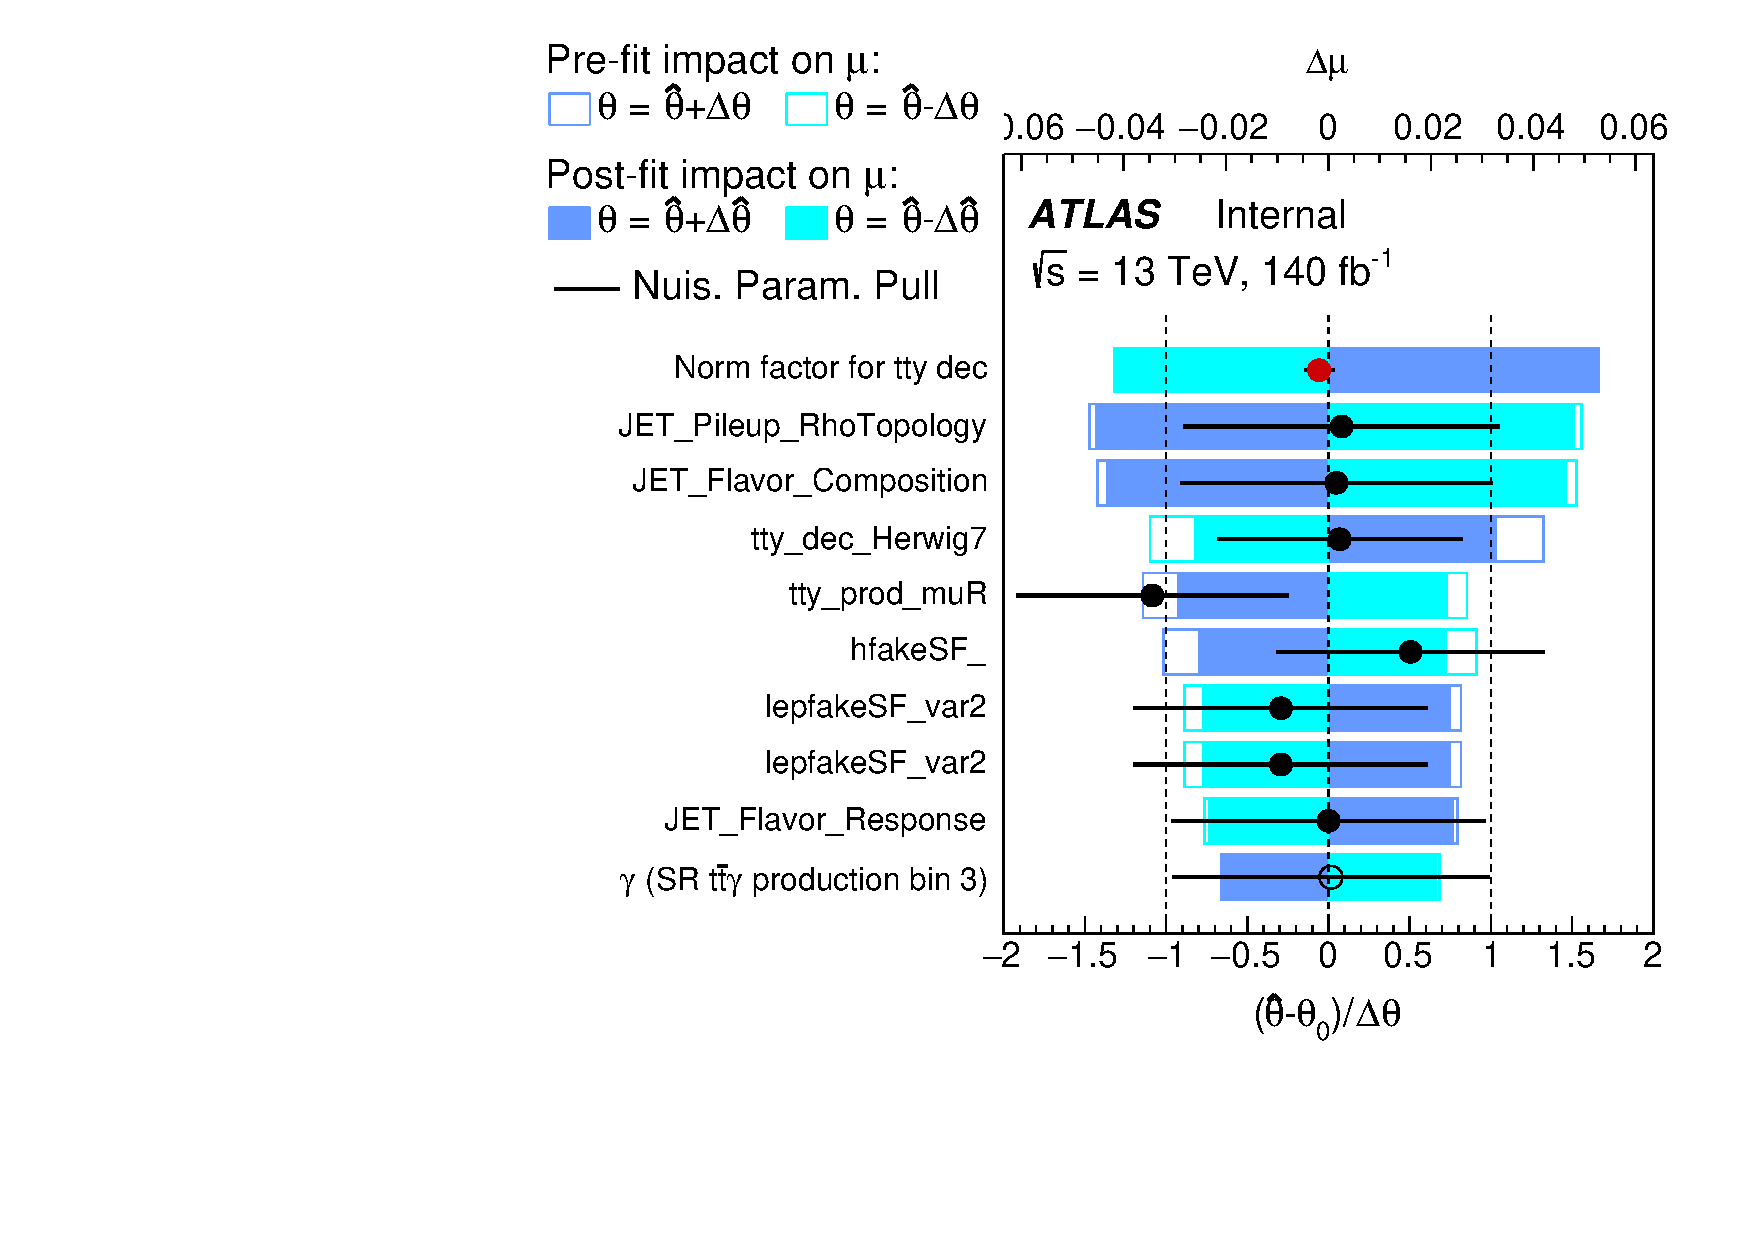
\includegraphics[width=0.2\textwidth]{figures/diff_xsec/ljet_tty_prod_mu_blinded/Ranking/tty1l_pt_all_syst/Ranking_tty_pt_Bin_004_mu.pdf}}
  \quad
  \subfloat[]{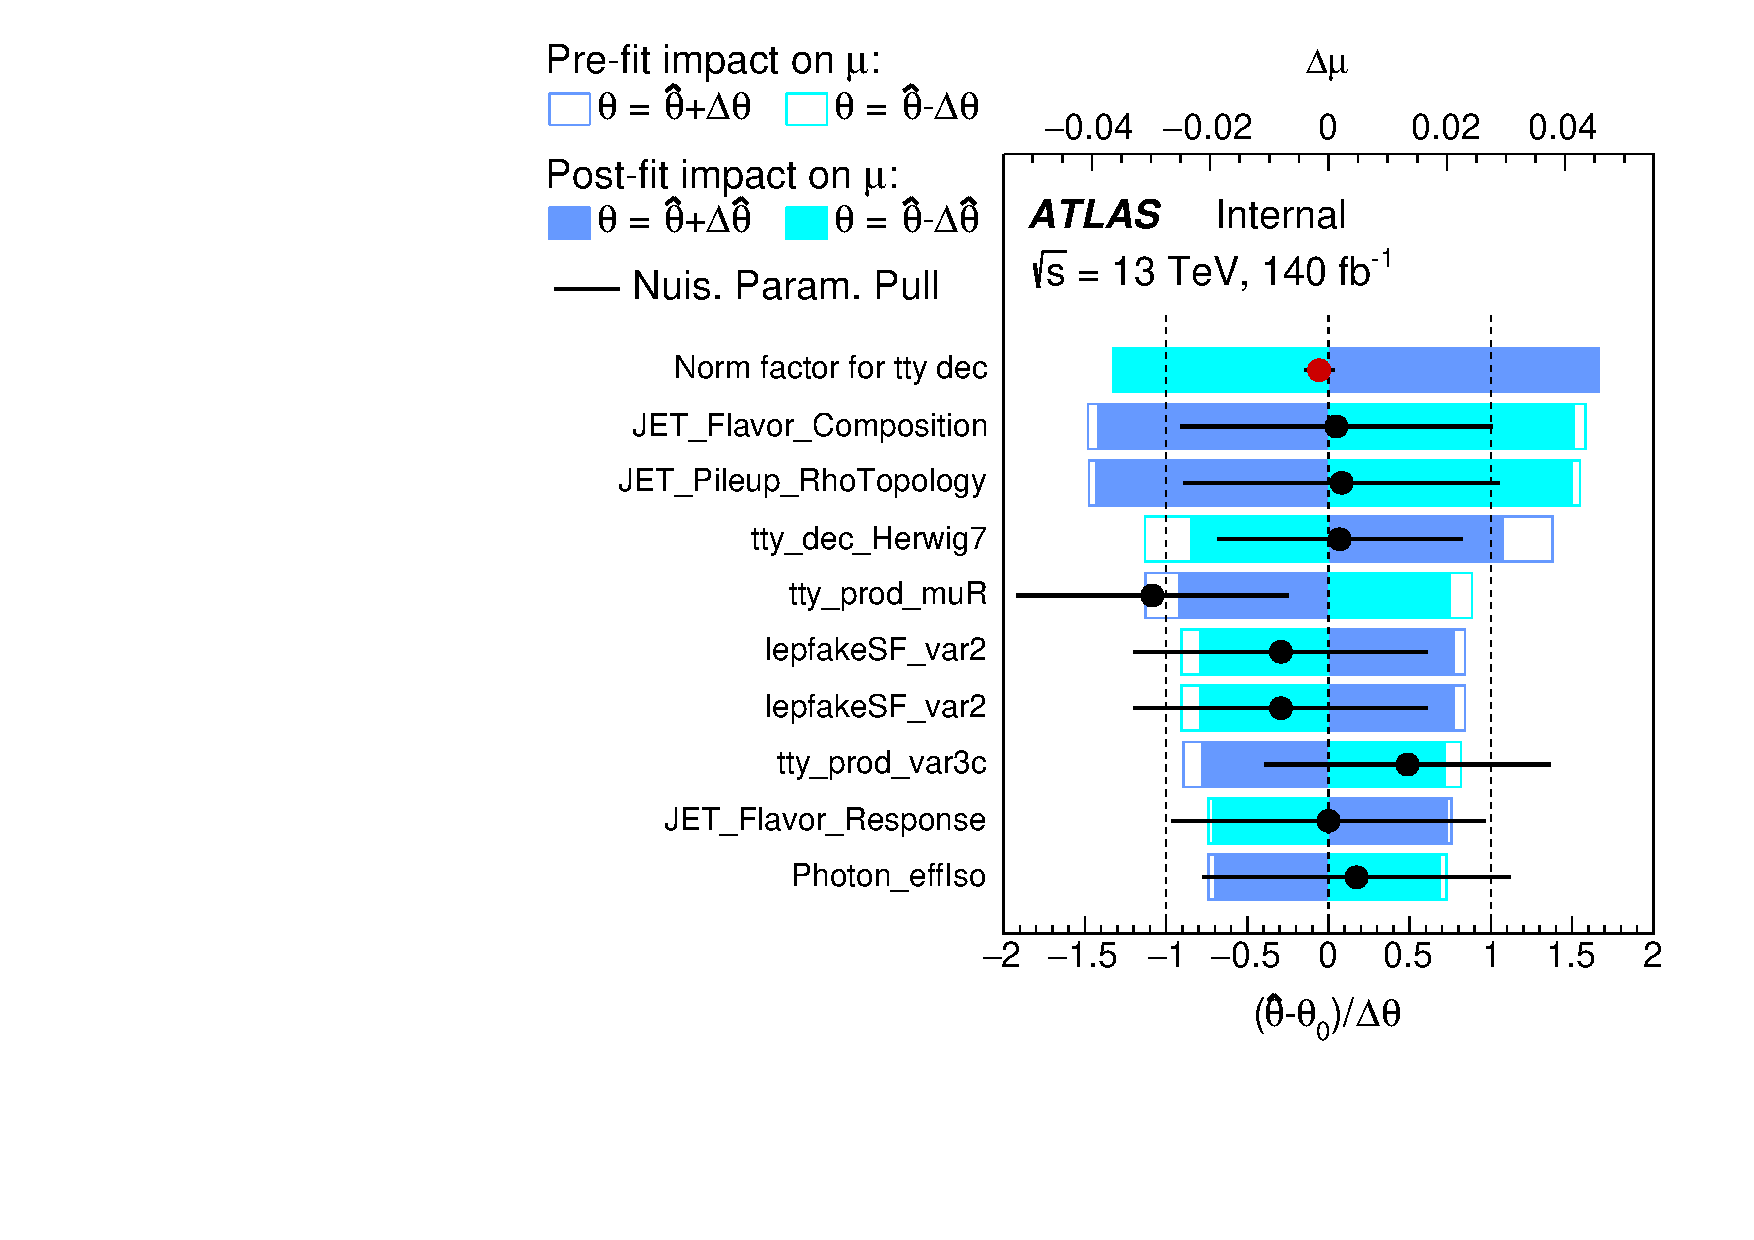
\includegraphics[width=0.2\textwidth]{figures/diff_xsec/ljet_tty_prod_mu_blinded/Ranking/tty1l_pt_all_syst/Ranking_tty_pt_Bin_005_mu.pdf}}
  \quad
  \subfloat[]{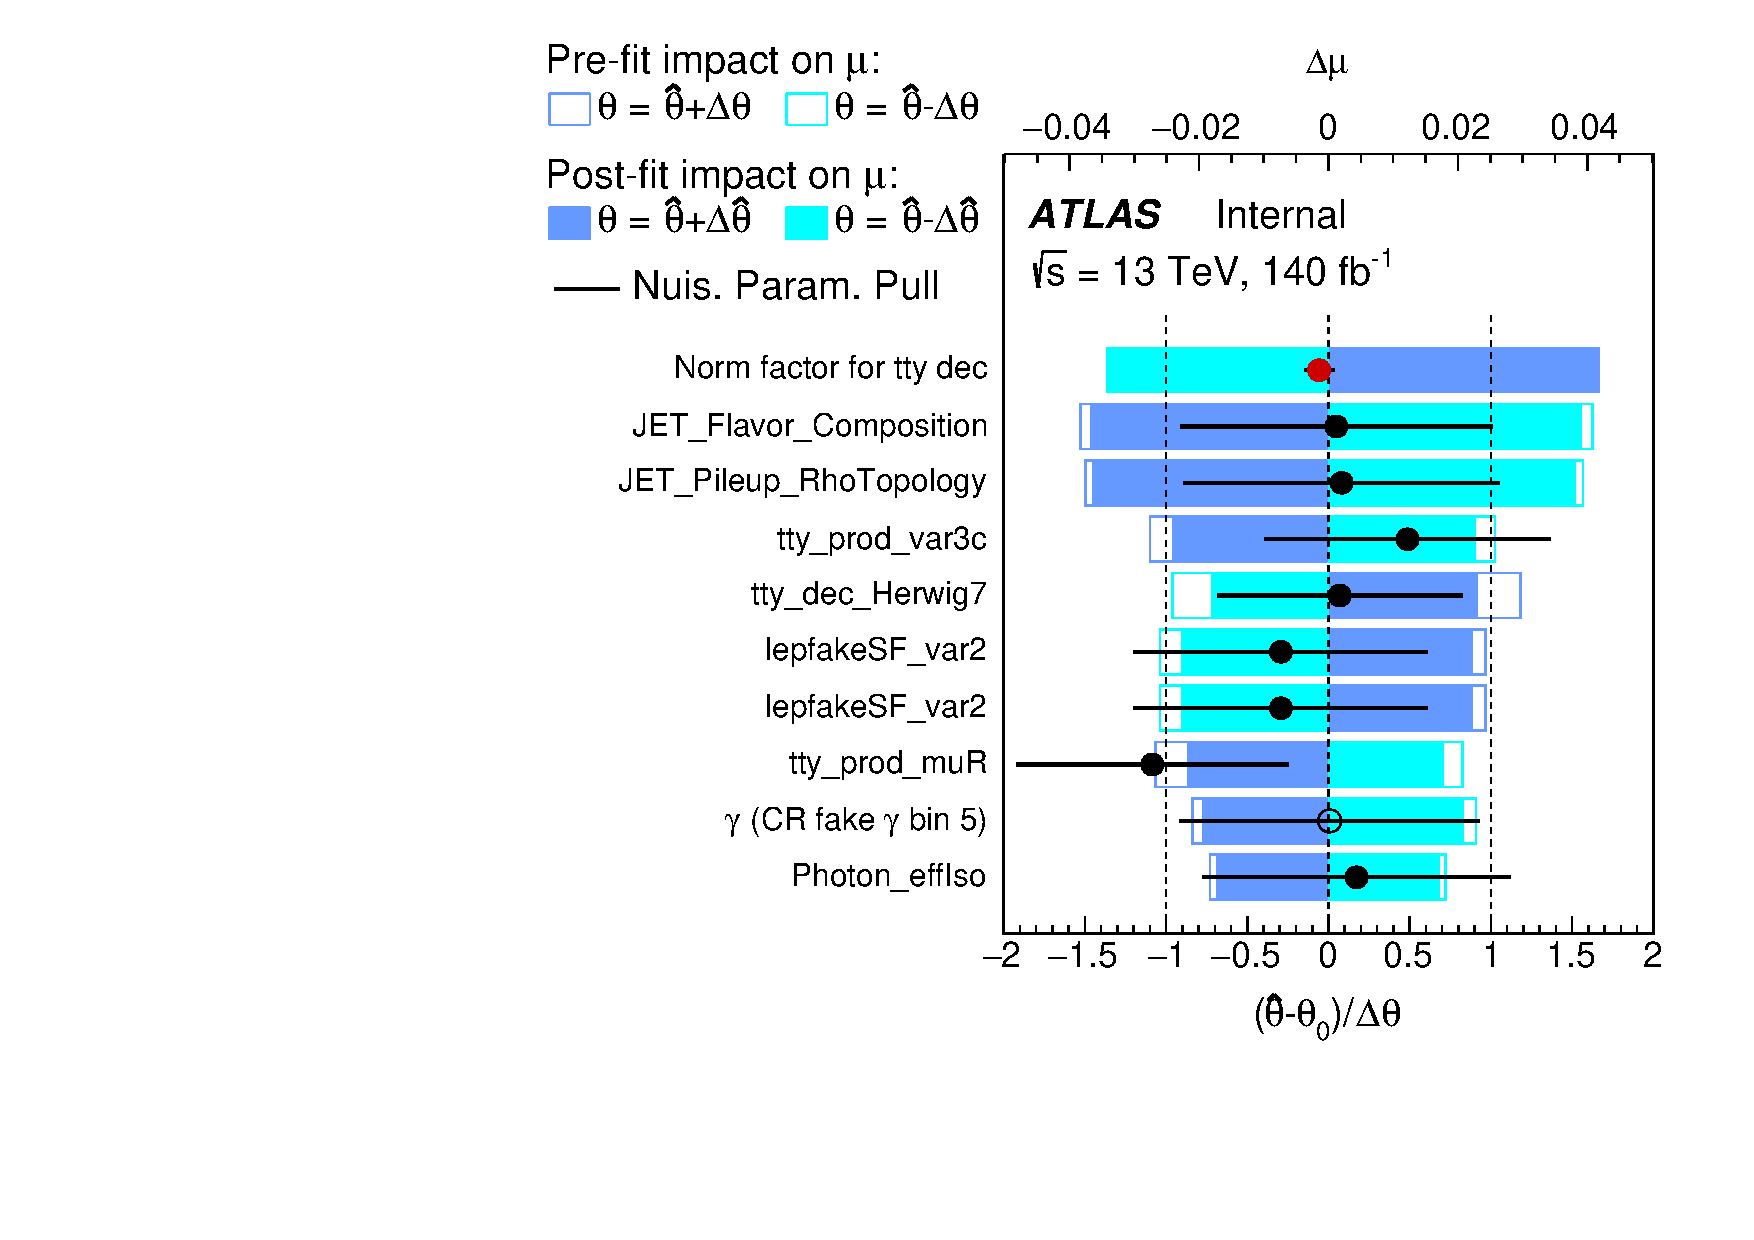
\includegraphics[width=0.2\textwidth]{figures/diff_xsec/ljet_tty_prod_mu_blinded/Ranking/tty1l_pt_all_syst/Ranking_tty_pt_Bin_006_mu.pdf}}
  \quad
  \subfloat[]{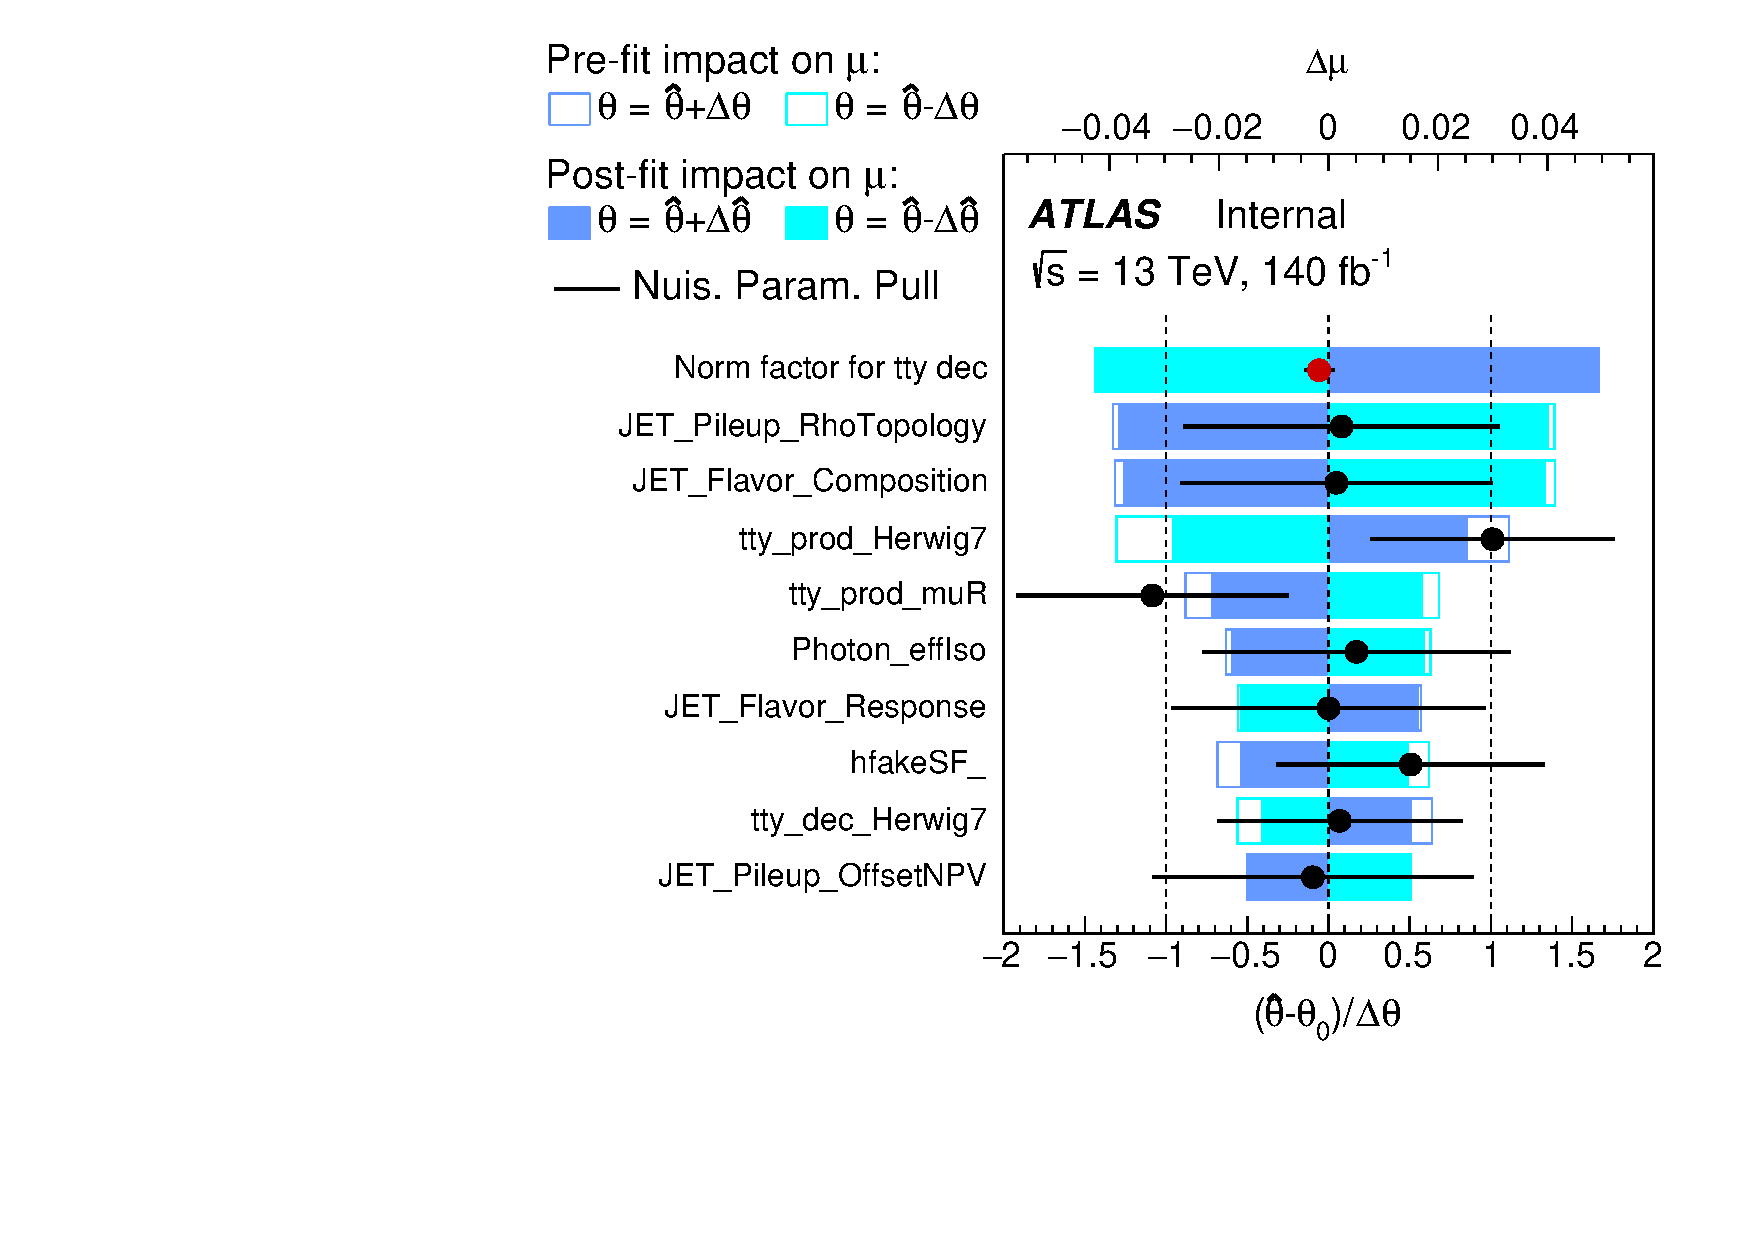
\includegraphics[width=0.2\textwidth]{figures/diff_xsec/ljet_tty_prod_mu_blinded/Ranking/tty1l_pt_all_syst/Ranking_tty_pt_Bin_007_mu.pdf}}
  \quad
  \subfloat[]{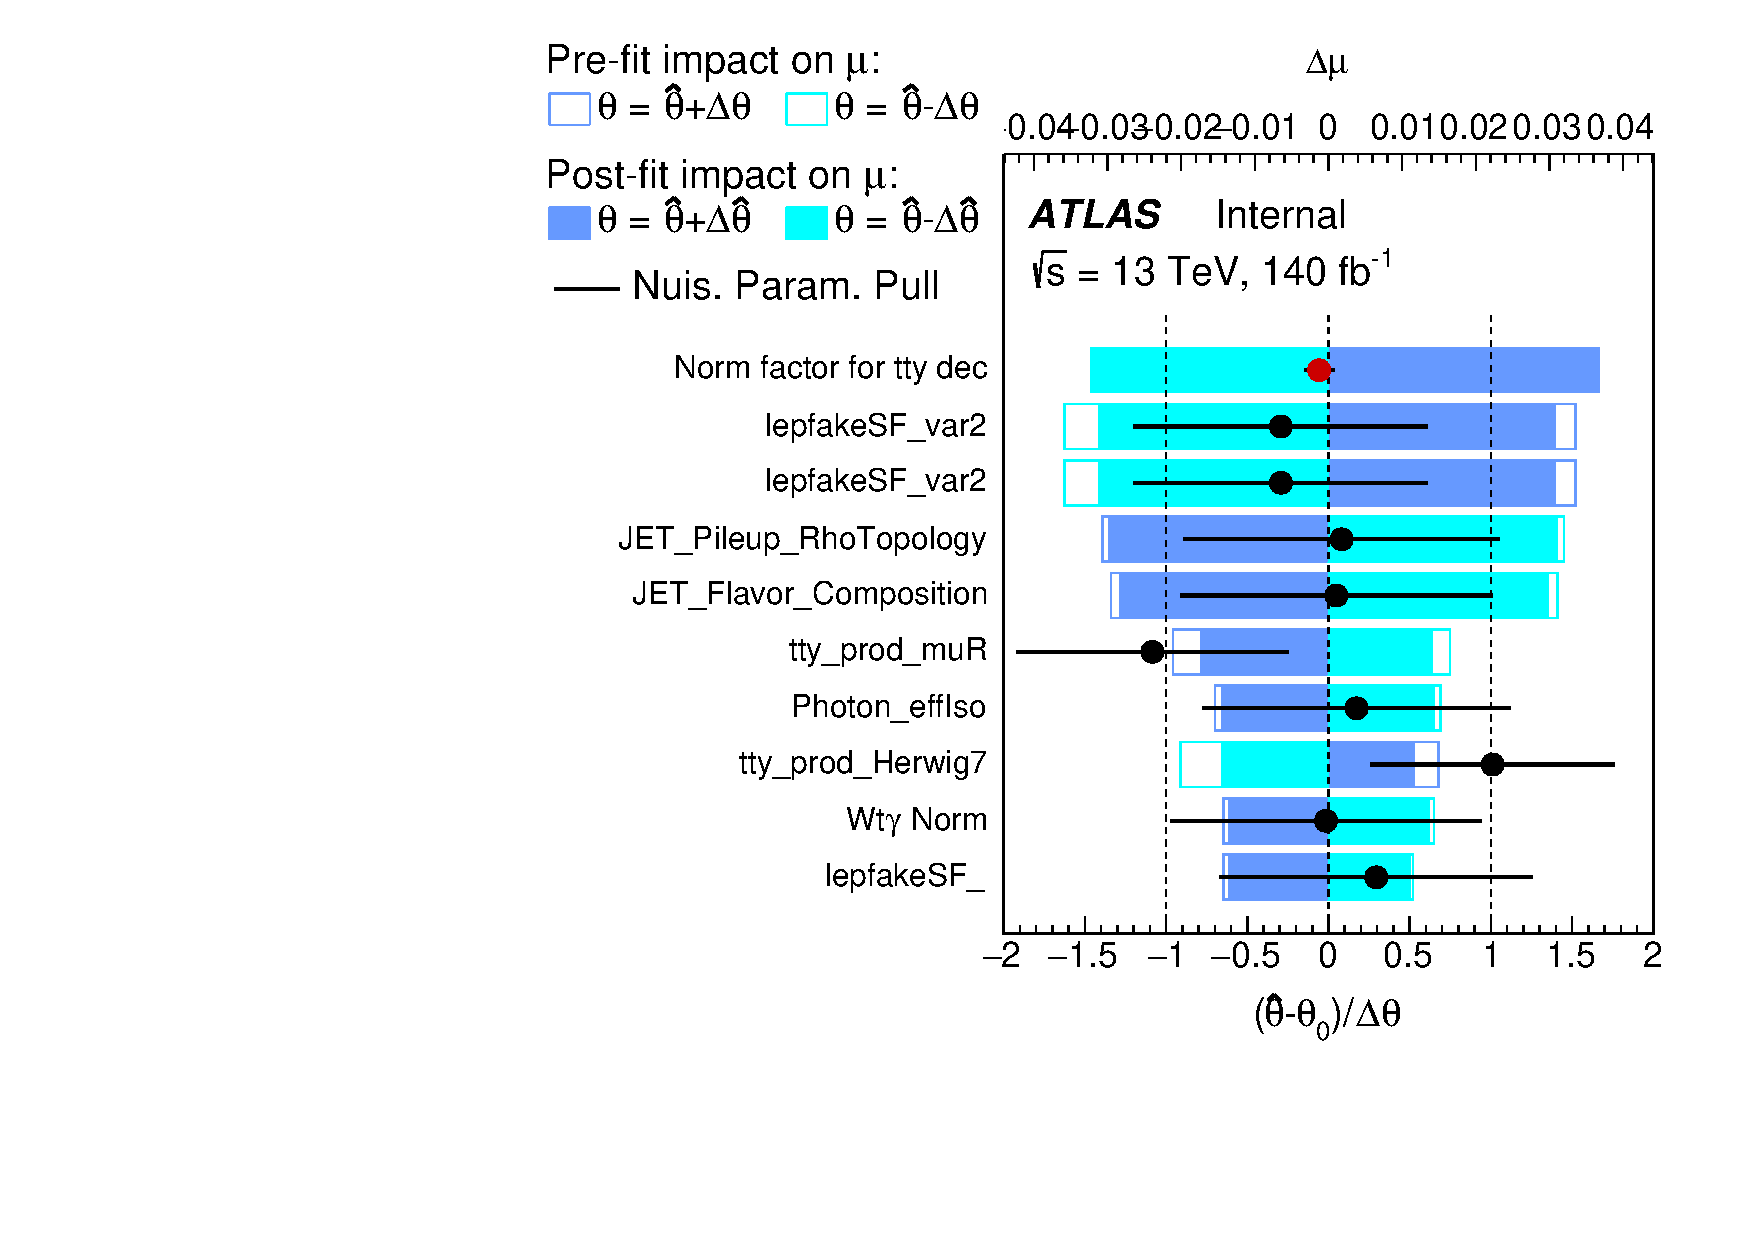
\includegraphics[width=0.2\textwidth]{figures/diff_xsec/ljet_tty_prod_mu_blinded/Ranking/tty1l_pt_all_syst/Ranking_tty_pt_Bin_008_mu.pdf}}
  \quad
  \subfloat[]{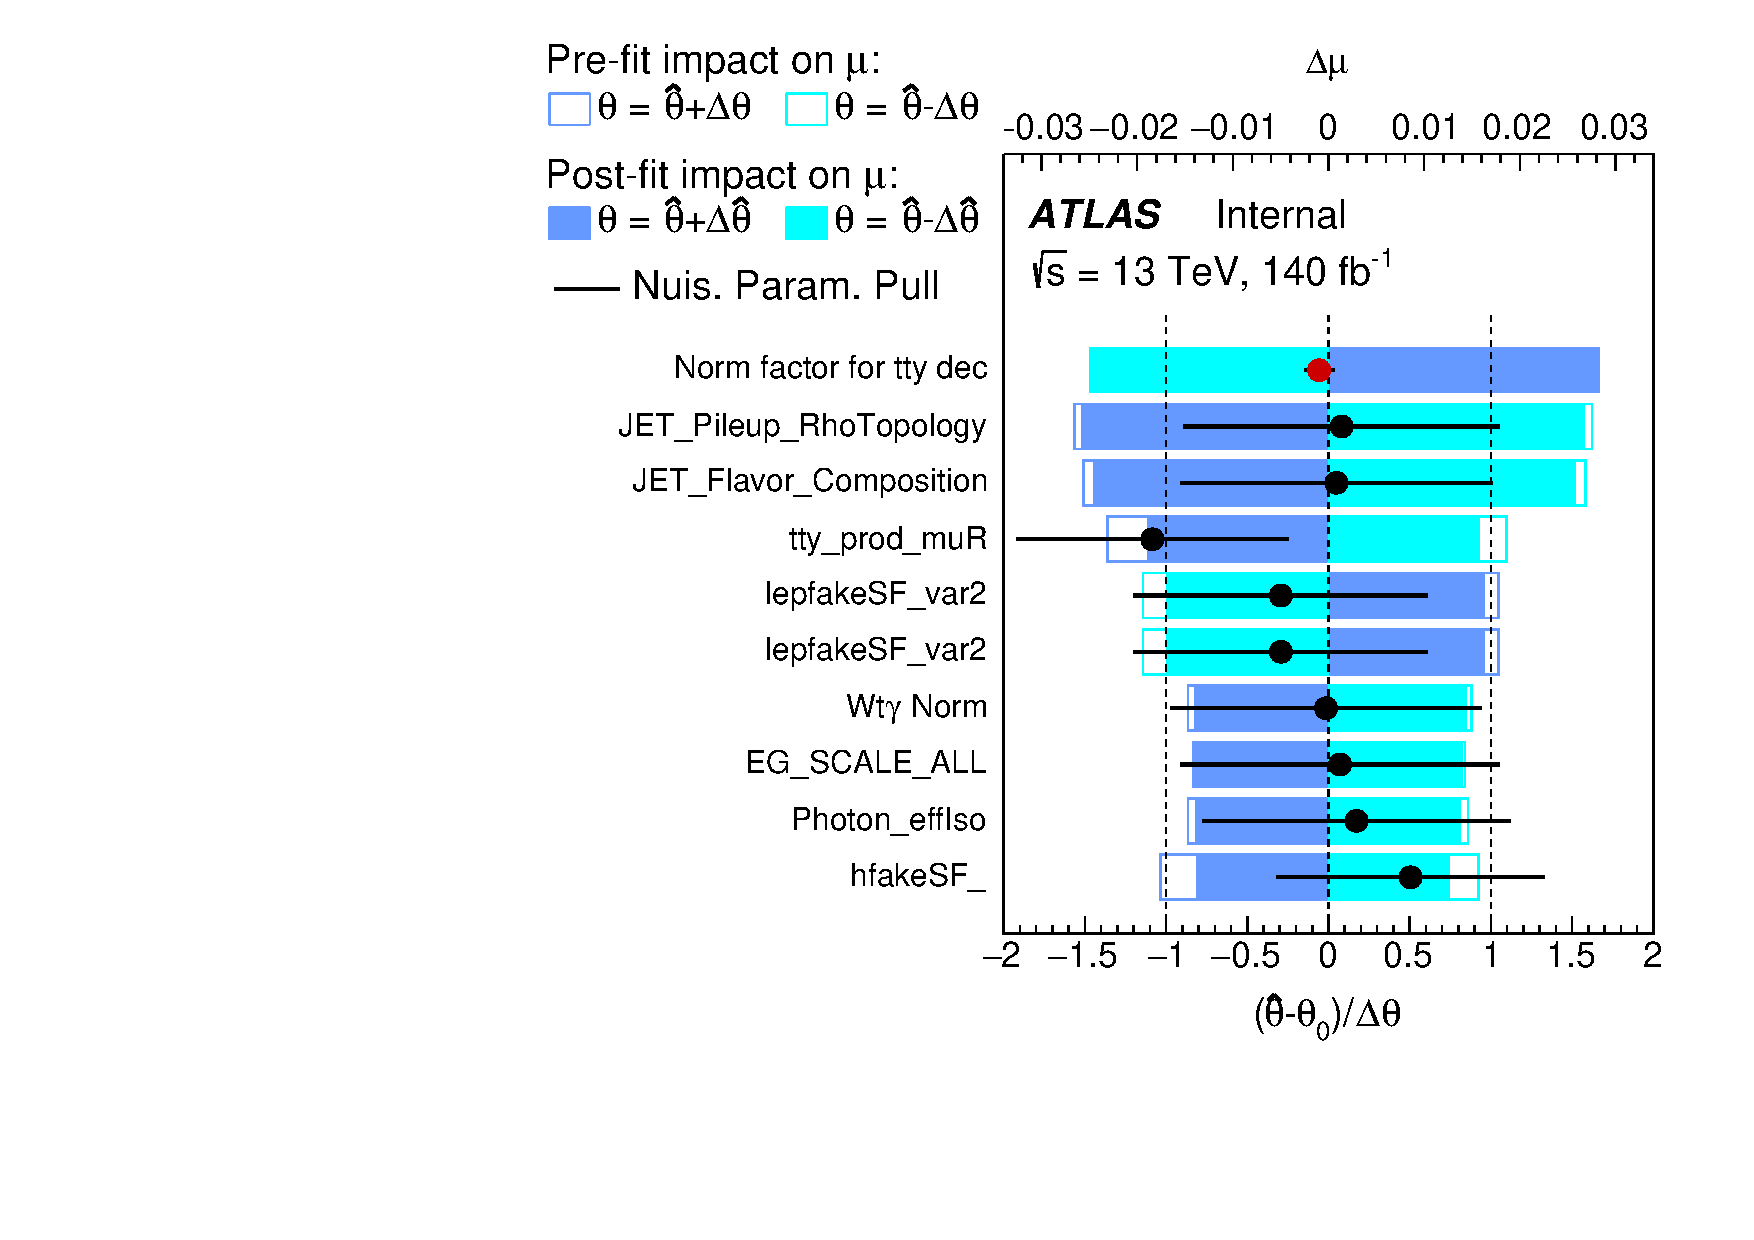
\includegraphics[width=0.2\textwidth]{figures/diff_xsec/ljet_tty_prod_mu_blinded/Ranking/tty1l_pt_all_syst/Ranking_tty_pt_Bin_009_mu.pdf}}
  \quad
  \subfloat[]{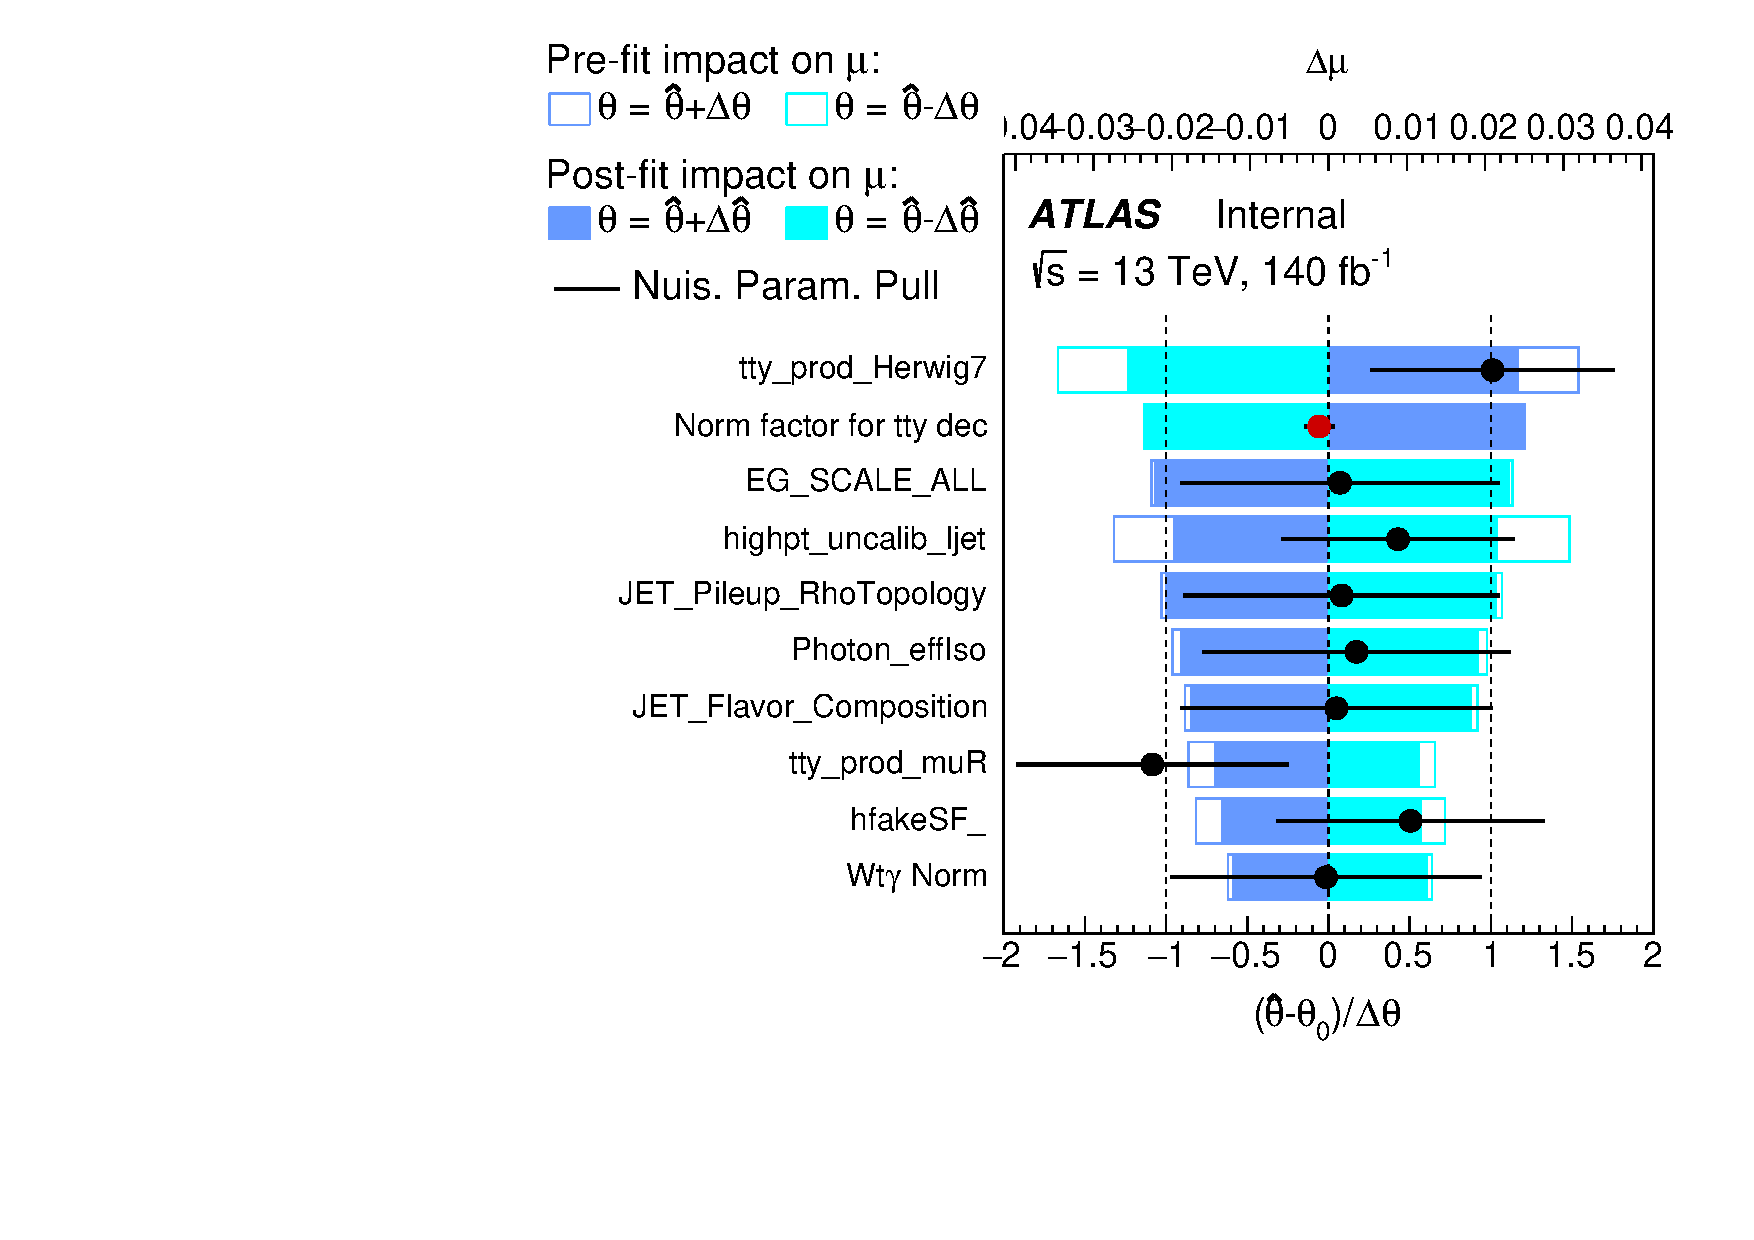
\includegraphics[width=0.2\textwidth]{figures/diff_xsec/ljet_tty_prod_mu_blinded/Ranking/tty1l_pt_all_syst/Ranking_tty_pt_Bin_010_mu.pdf}}
  \quad

  \caption{Ranking plots of the 10 NPs with the largest impact on the \tty (prod) singal strength in each bin of the $p_T(\gamma)$ distribution in the single 
  lepton channel. The fit was performed to the real dataset. Each subfigure, labeled (a), (b), (c), (d), ... (j), corresponds to a specific bin 
  of the $p_T(\gamma)$ distribution, with bin 1 represented in subfigure (a), bin 2 represented in 
  subfigure (b), and so on.}
  \label{fig:ranking_ljet_total}
\end{figure}
\FloatBarrier


\begin{figure}[ht]
  \centering
  \subfloat[]{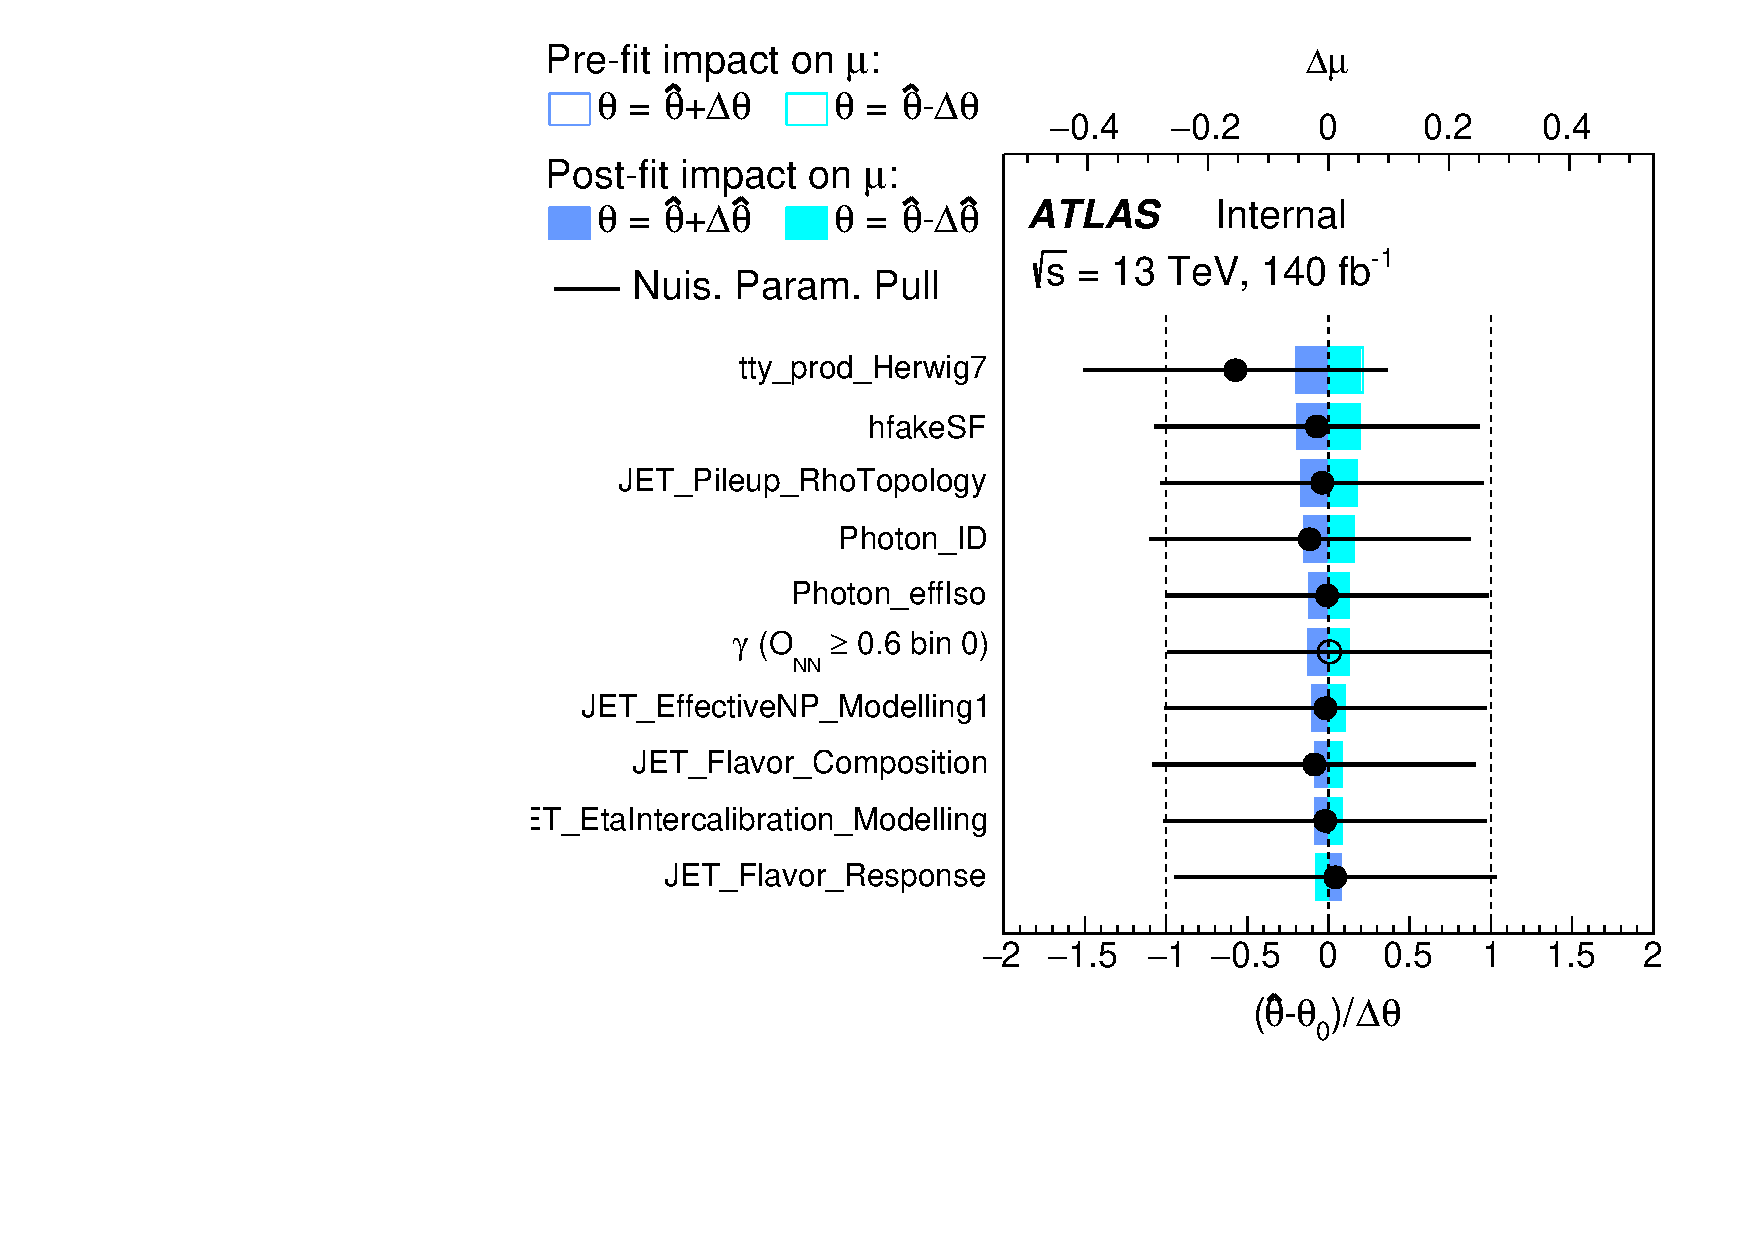
\includegraphics[width=0.2\textwidth]{figures/diff_xsec/dilep_tty_prod_mu_blinded/Ranking/tty2l_pt_all_syst/Ranking_tty_pt_Bin_001_mu.pdf}}
  \quad
  \subfloat[]{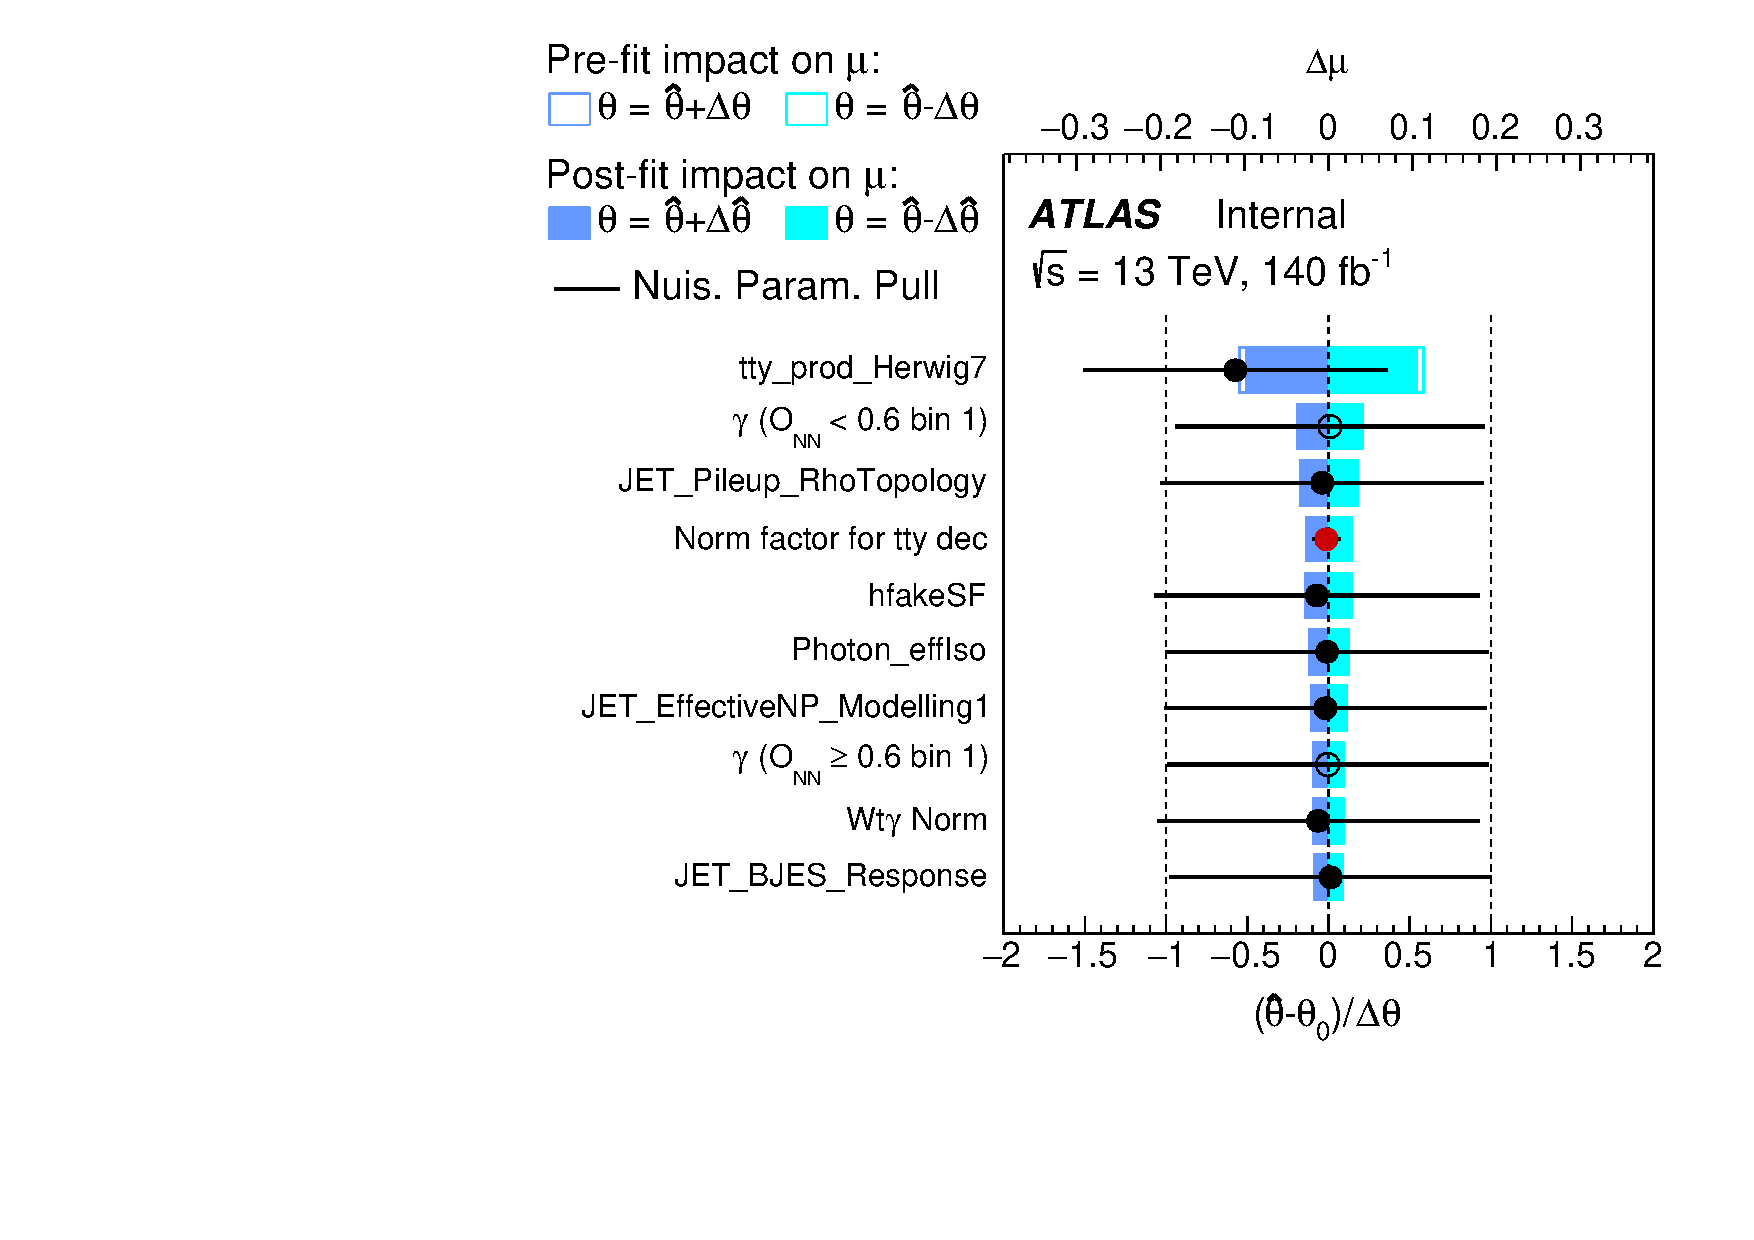
\includegraphics[width=0.2\textwidth]{figures/diff_xsec/dilep_tty_prod_mu_blinded/Ranking/tty2l_pt_all_syst/Ranking_tty_pt_Bin_002_mu.pdf}}
  \quad
  \subfloat[]{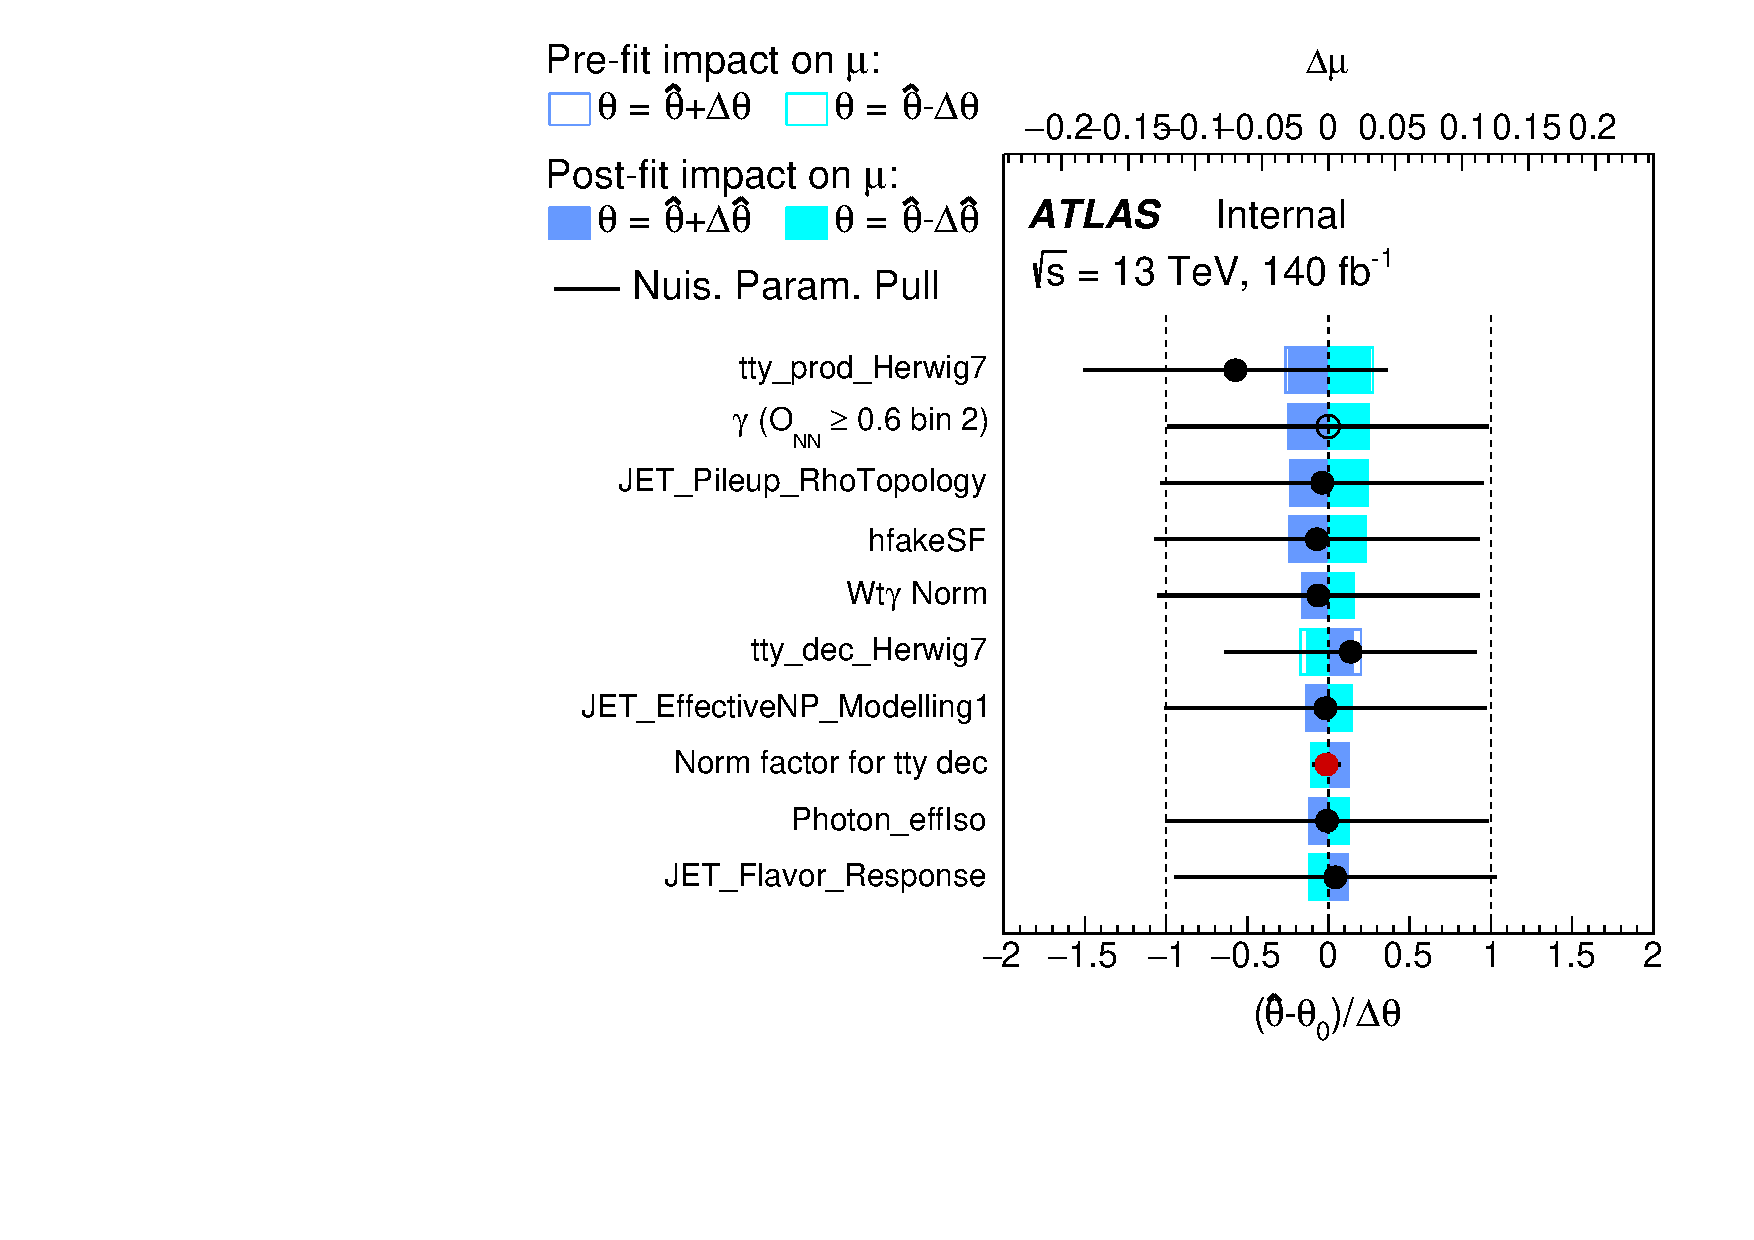
\includegraphics[width=0.2\textwidth]{figures/diff_xsec/dilep_tty_prod_mu_blinded/Ranking/tty2l_pt_all_syst/Ranking_tty_pt_Bin_003_mu.pdf}}
  \quad
  \subfloat[]{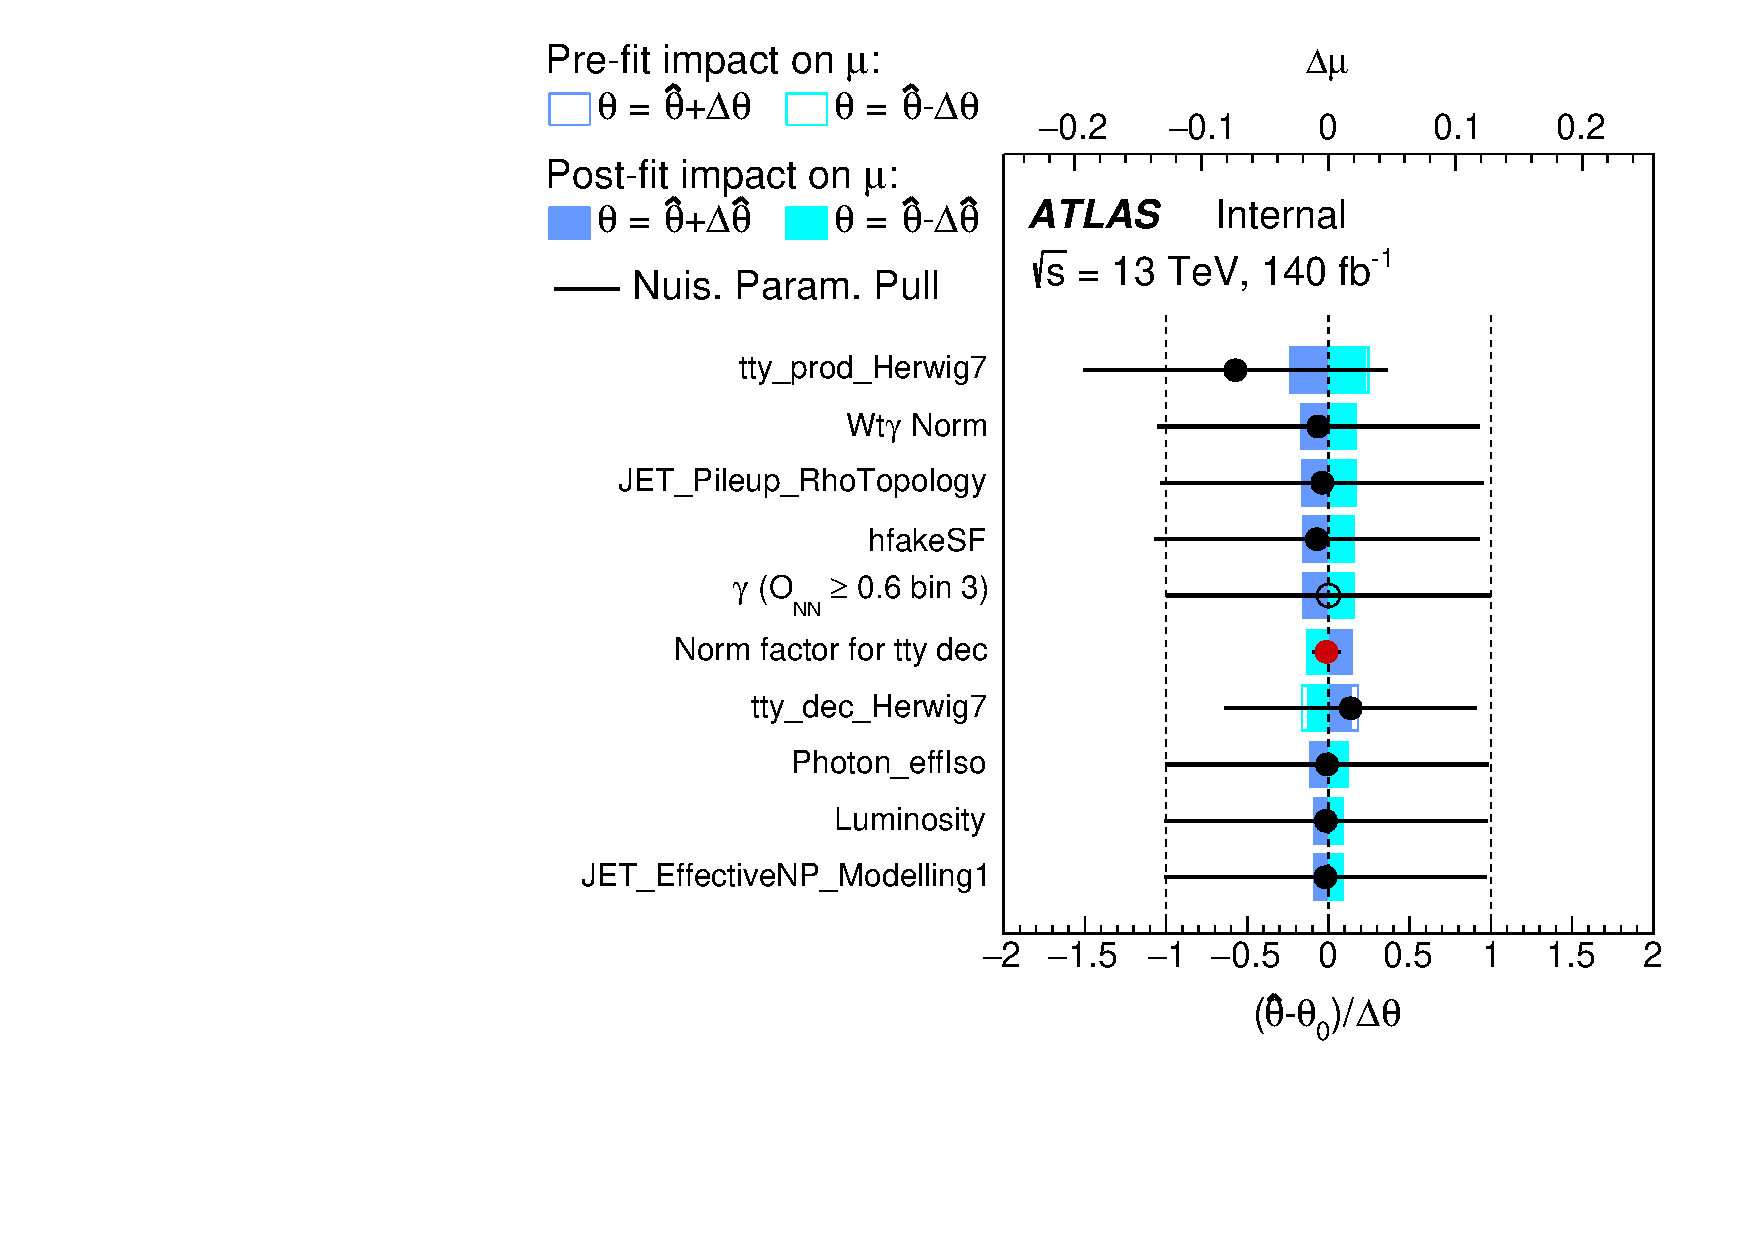
\includegraphics[width=0.2\textwidth]{figures/diff_xsec/dilep_tty_prod_mu_blinded/Ranking/tty2l_pt_all_syst/Ranking_tty_pt_Bin_004_mu.pdf}}
  \quad
  \subfloat[]{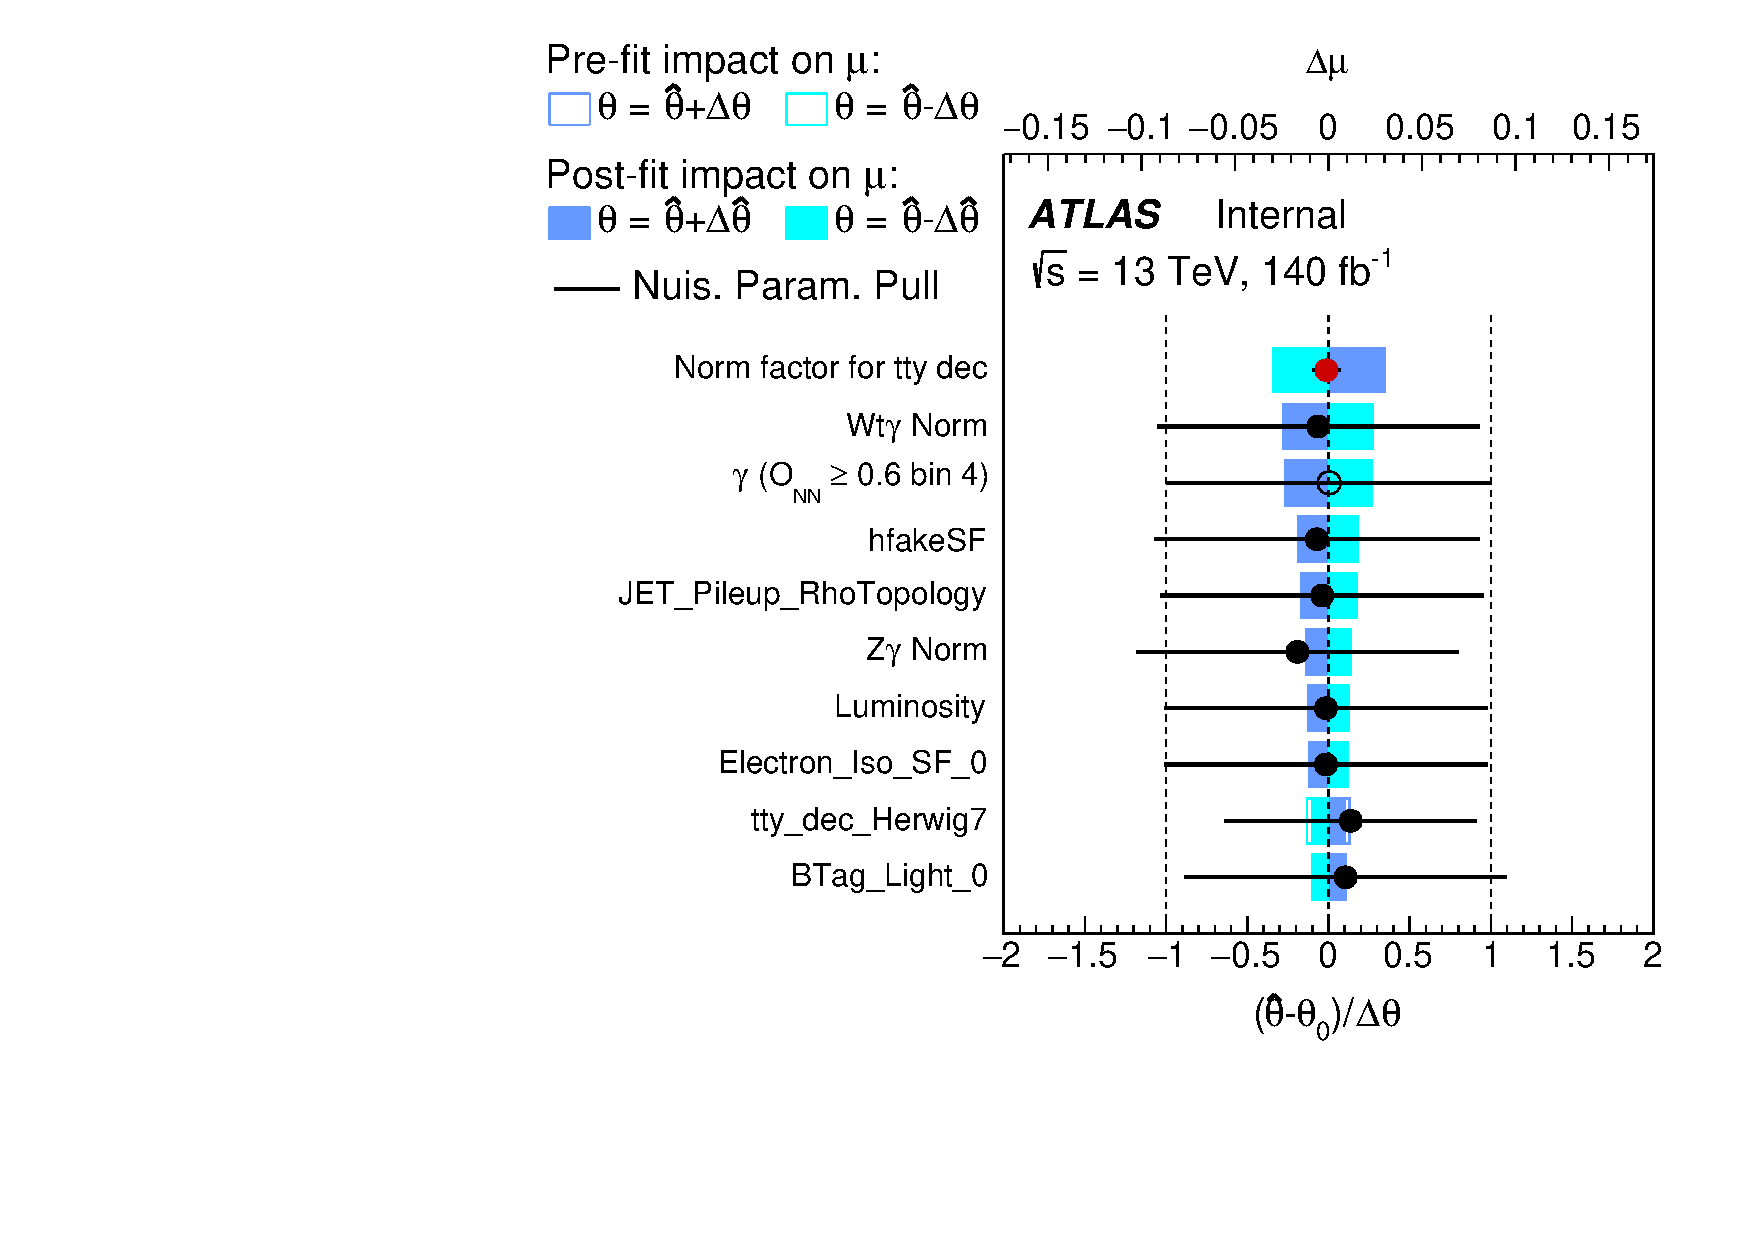
\includegraphics[width=0.2\textwidth]{figures/diff_xsec/dilep_tty_prod_mu_blinded/Ranking/tty2l_pt_all_syst/Ranking_tty_pt_Bin_005_mu.pdf}}
  \quad
  \subfloat[]{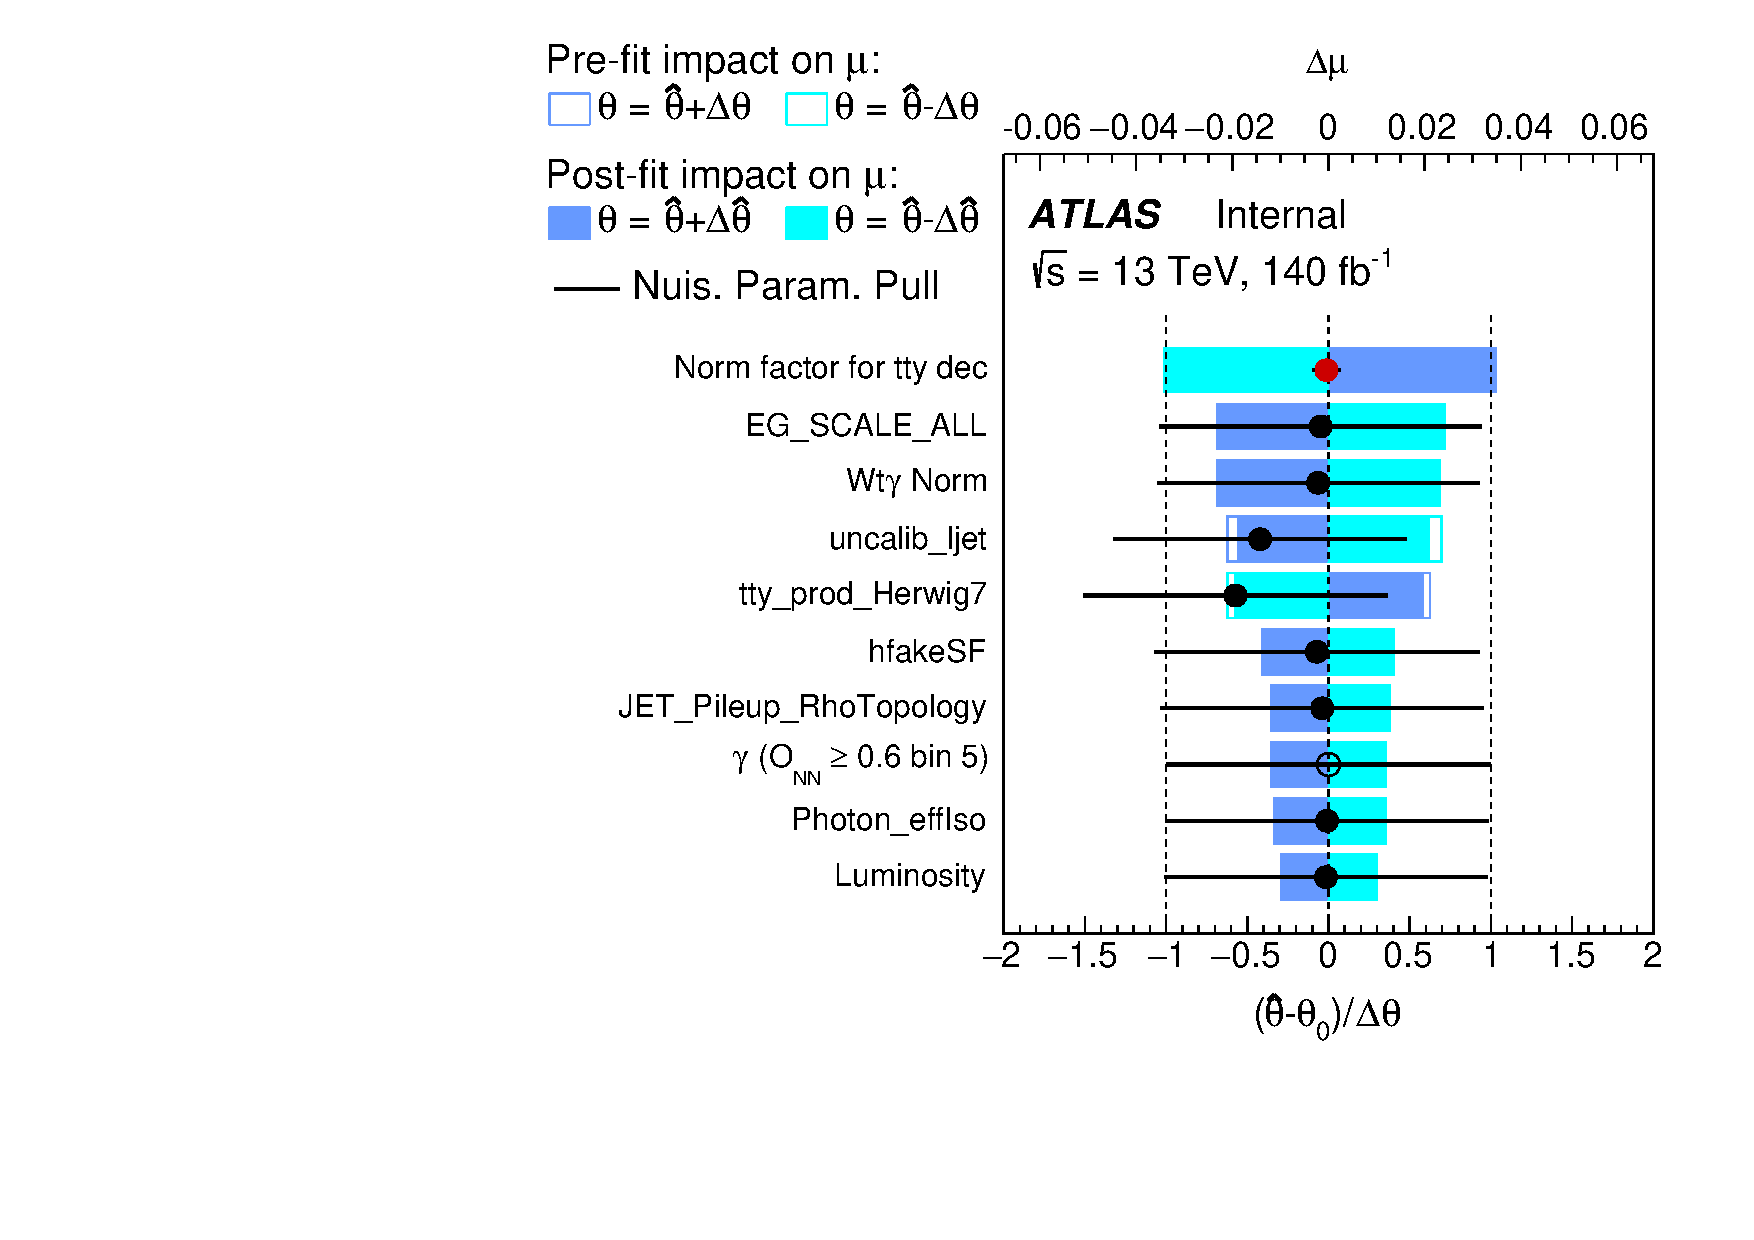
\includegraphics[width=0.2\textwidth]{figures/diff_xsec/dilep_tty_prod_mu_blinded/Ranking/tty2l_pt_all_syst/Ranking_tty_pt_Bin_006_mu.pdf}}
  \caption{Ranking plots of the 10 NPs with the largest impact on the \tty (prod) signal strength in each bin of the $p_T(\gamma)$ distribution in the dilepton channel. 
  The fit was performed to the real dataset. Each subfigure, labeled (a), (b), (c), (d), (e), and (f), corresponds to a specific bin 
  of the $p_T(\gamma)$ distribution, with bin 1 (lowest \pt) represented in subfigure (a), bin 2 represented in 
  subfigure (b), and so on. }
  \label{fig:ranking_dilep_total}
\end{figure}
\FloatBarrier

\begin{figure}[ht]
  \centering
  \subfloat[]{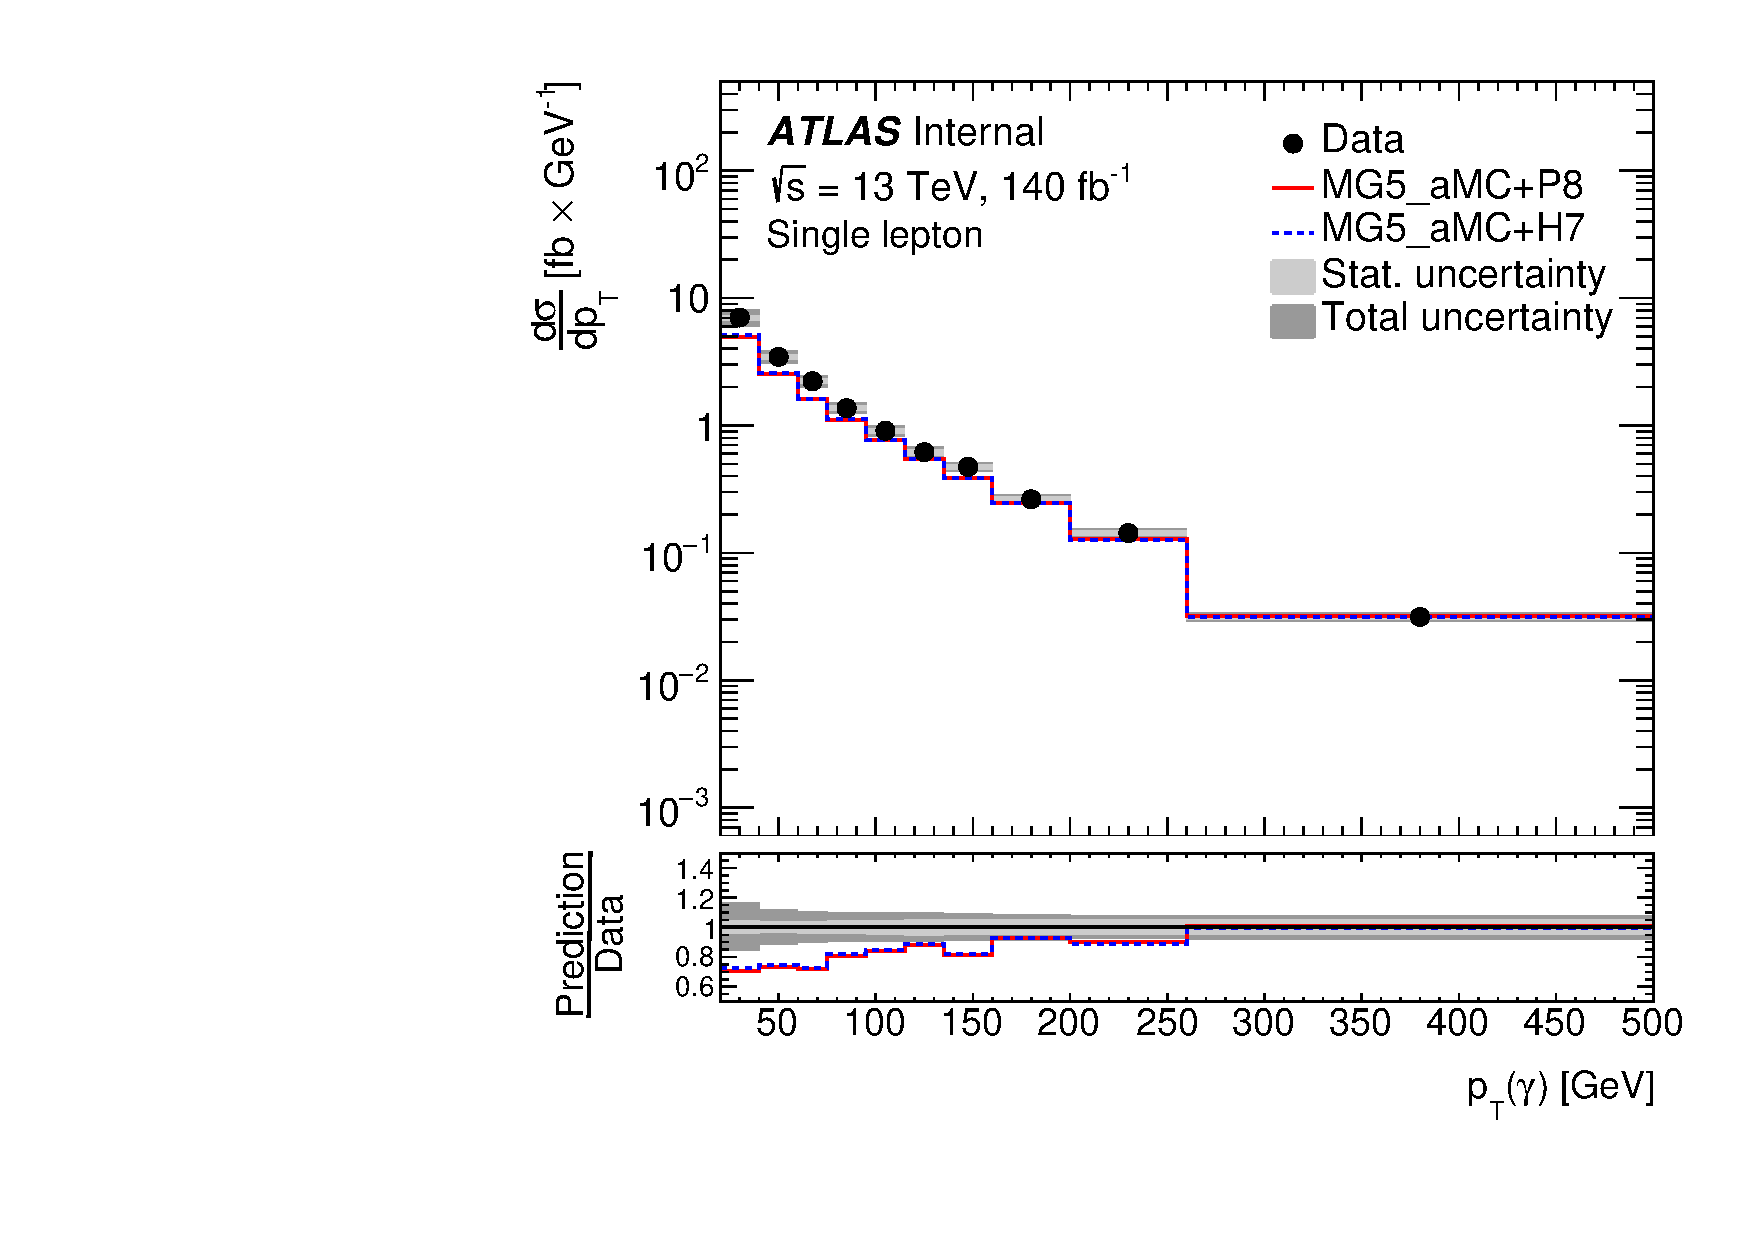
\includegraphics[width=0.4\textwidth]{figures/diff_xsec/absolute-unfolded-distributions/tty_prod_ljet/SL_tty_prod_pt_unfolded_absolute.pdf}}
  \quad\quad
  \subfloat[]{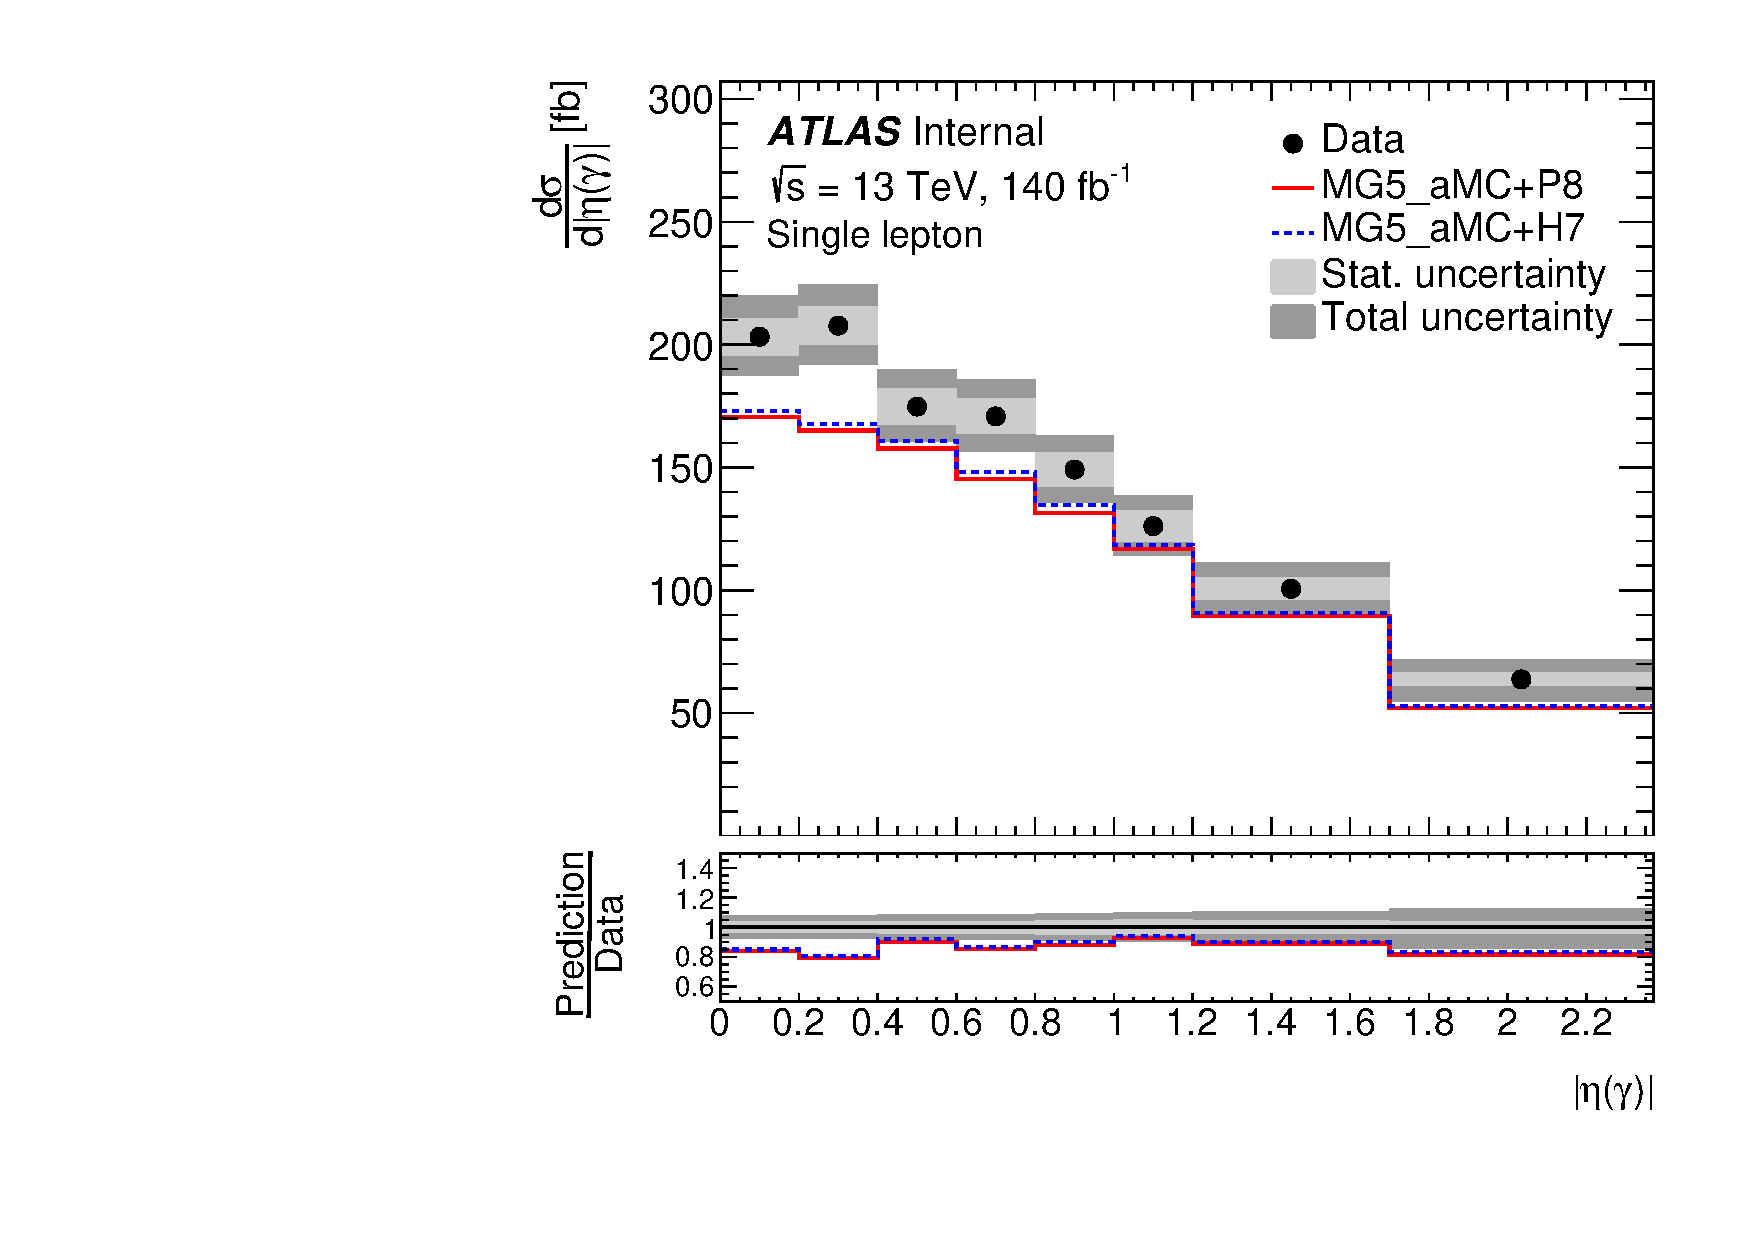
\includegraphics[width=0.4\textwidth]{figures/diff_xsec/absolute-unfolded-distributions/tty_prod_ljet/SL_tty_prod_eta_unfolded_absolute.pdf}}
  \quad\quad
  \subfloat[]{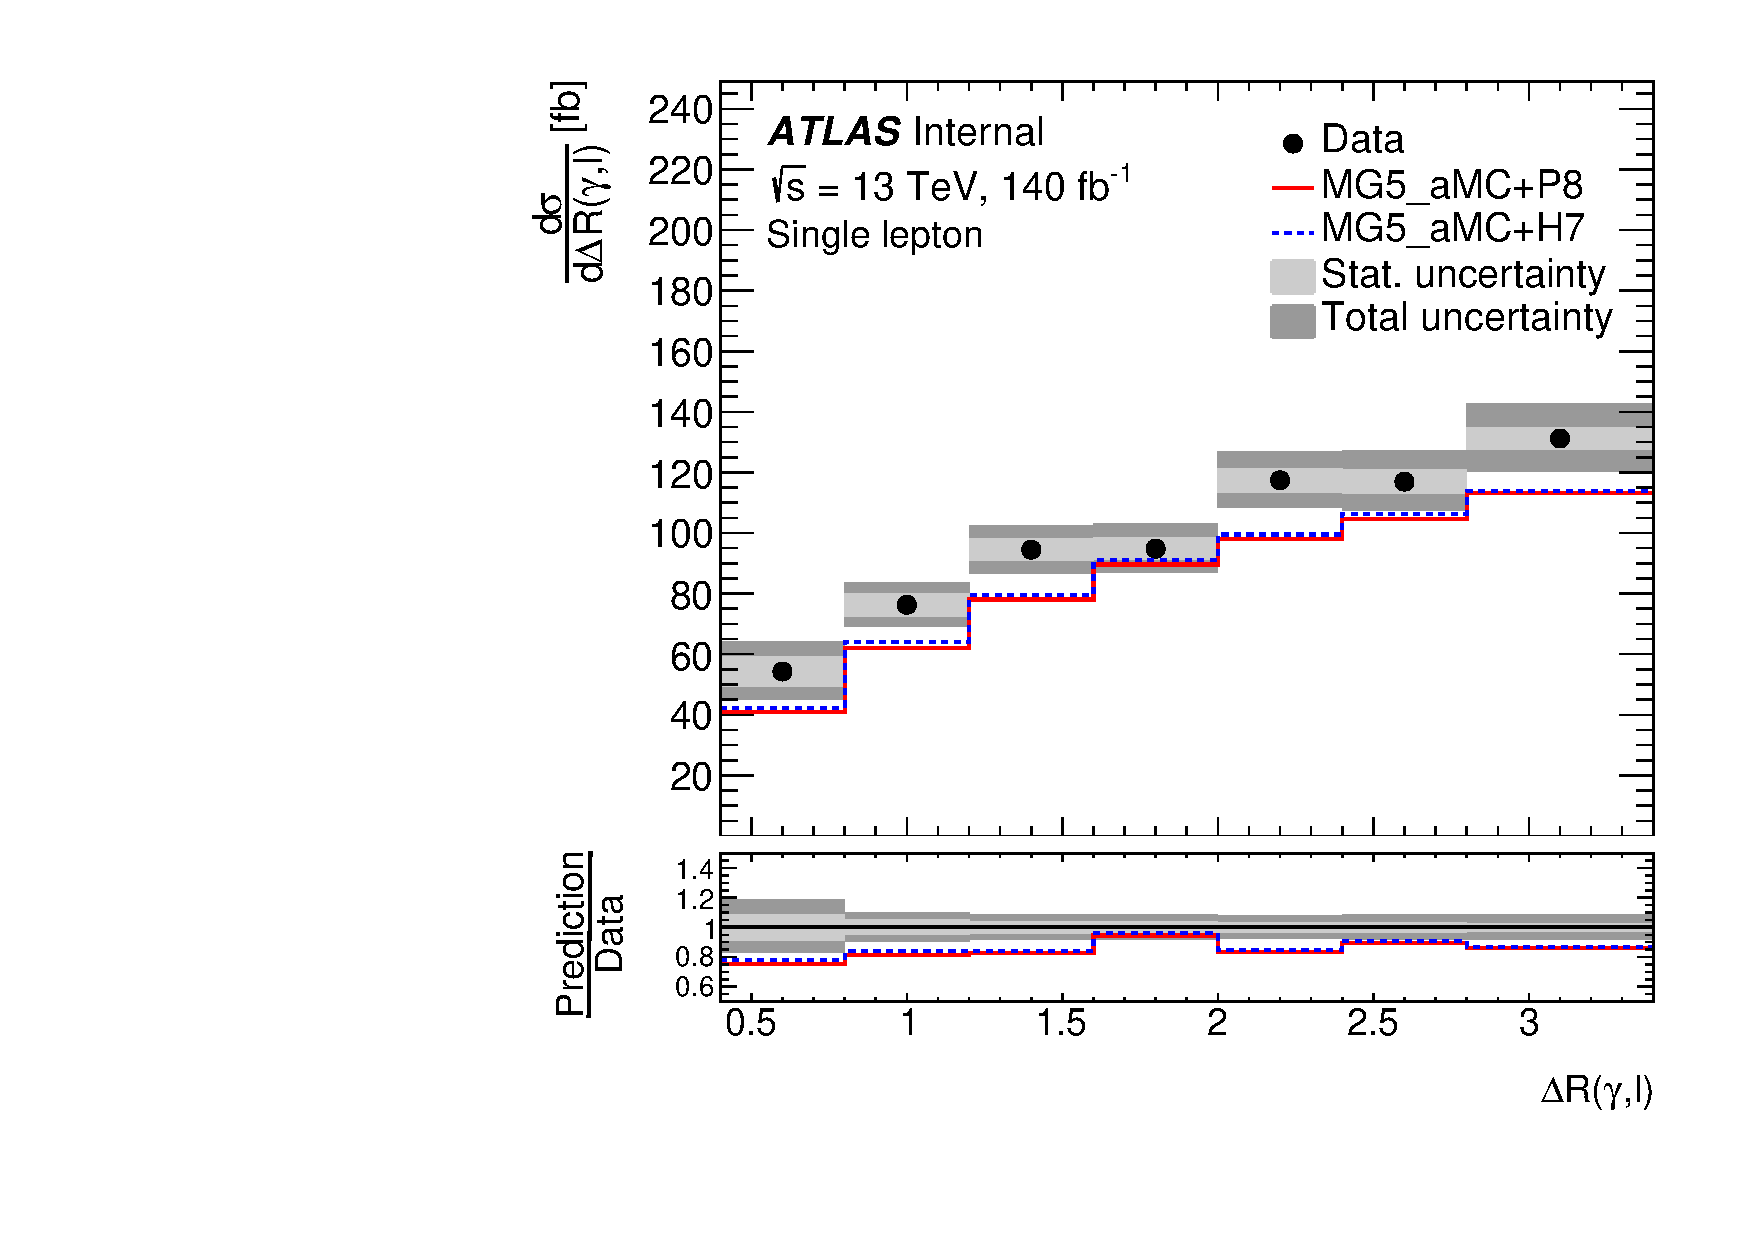
\includegraphics[width=0.4\textwidth]{figures/diff_xsec/absolute-unfolded-distributions/tty_prod_ljet/SL_tty_prod_drphl_unfolded_absolute.pdf}}
  \quad\quad
  \subfloat[]{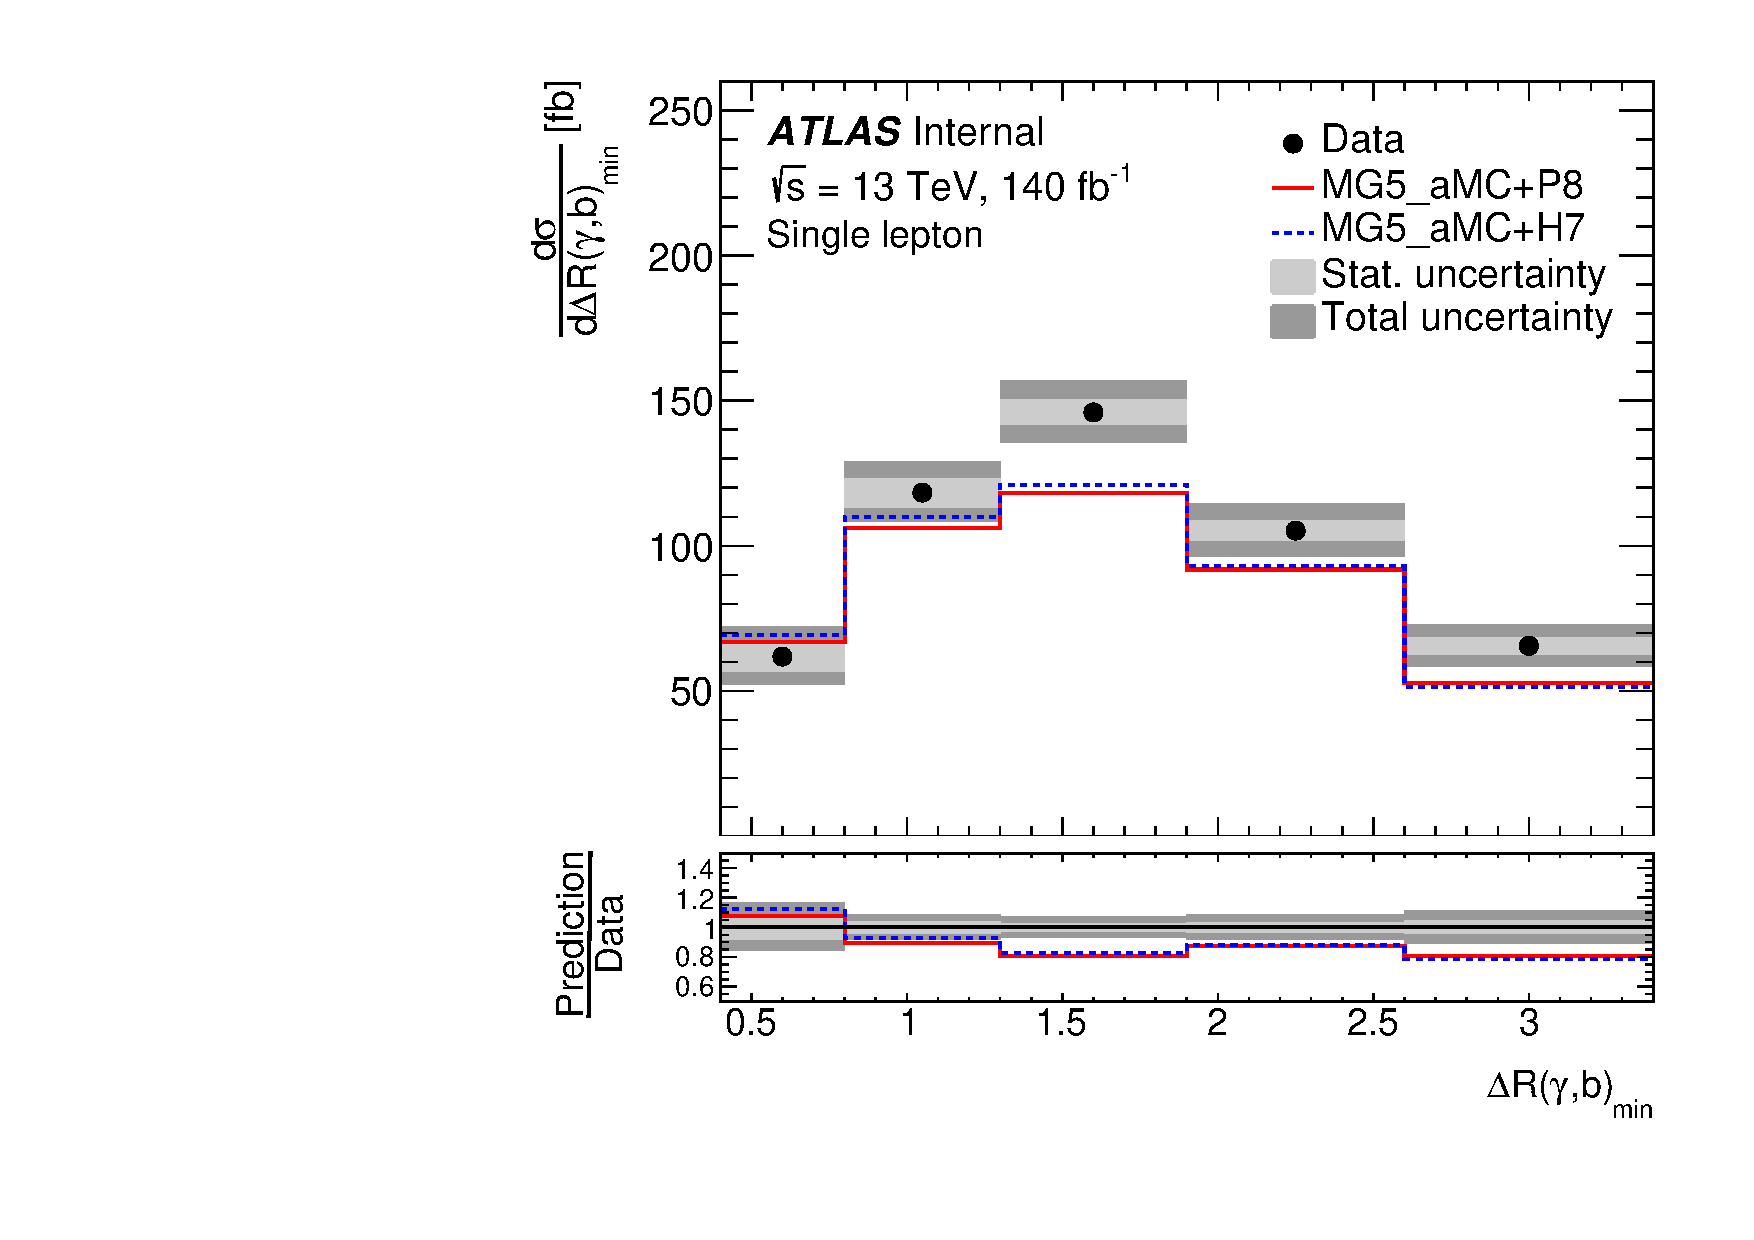
\includegraphics[width=0.4\textwidth]{figures/diff_xsec/absolute-unfolded-distributions/tty_prod_ljet/SL_tty_prod_drphb_unfolded_absolute.pdf}}
  \quad\quad
  \subfloat[]{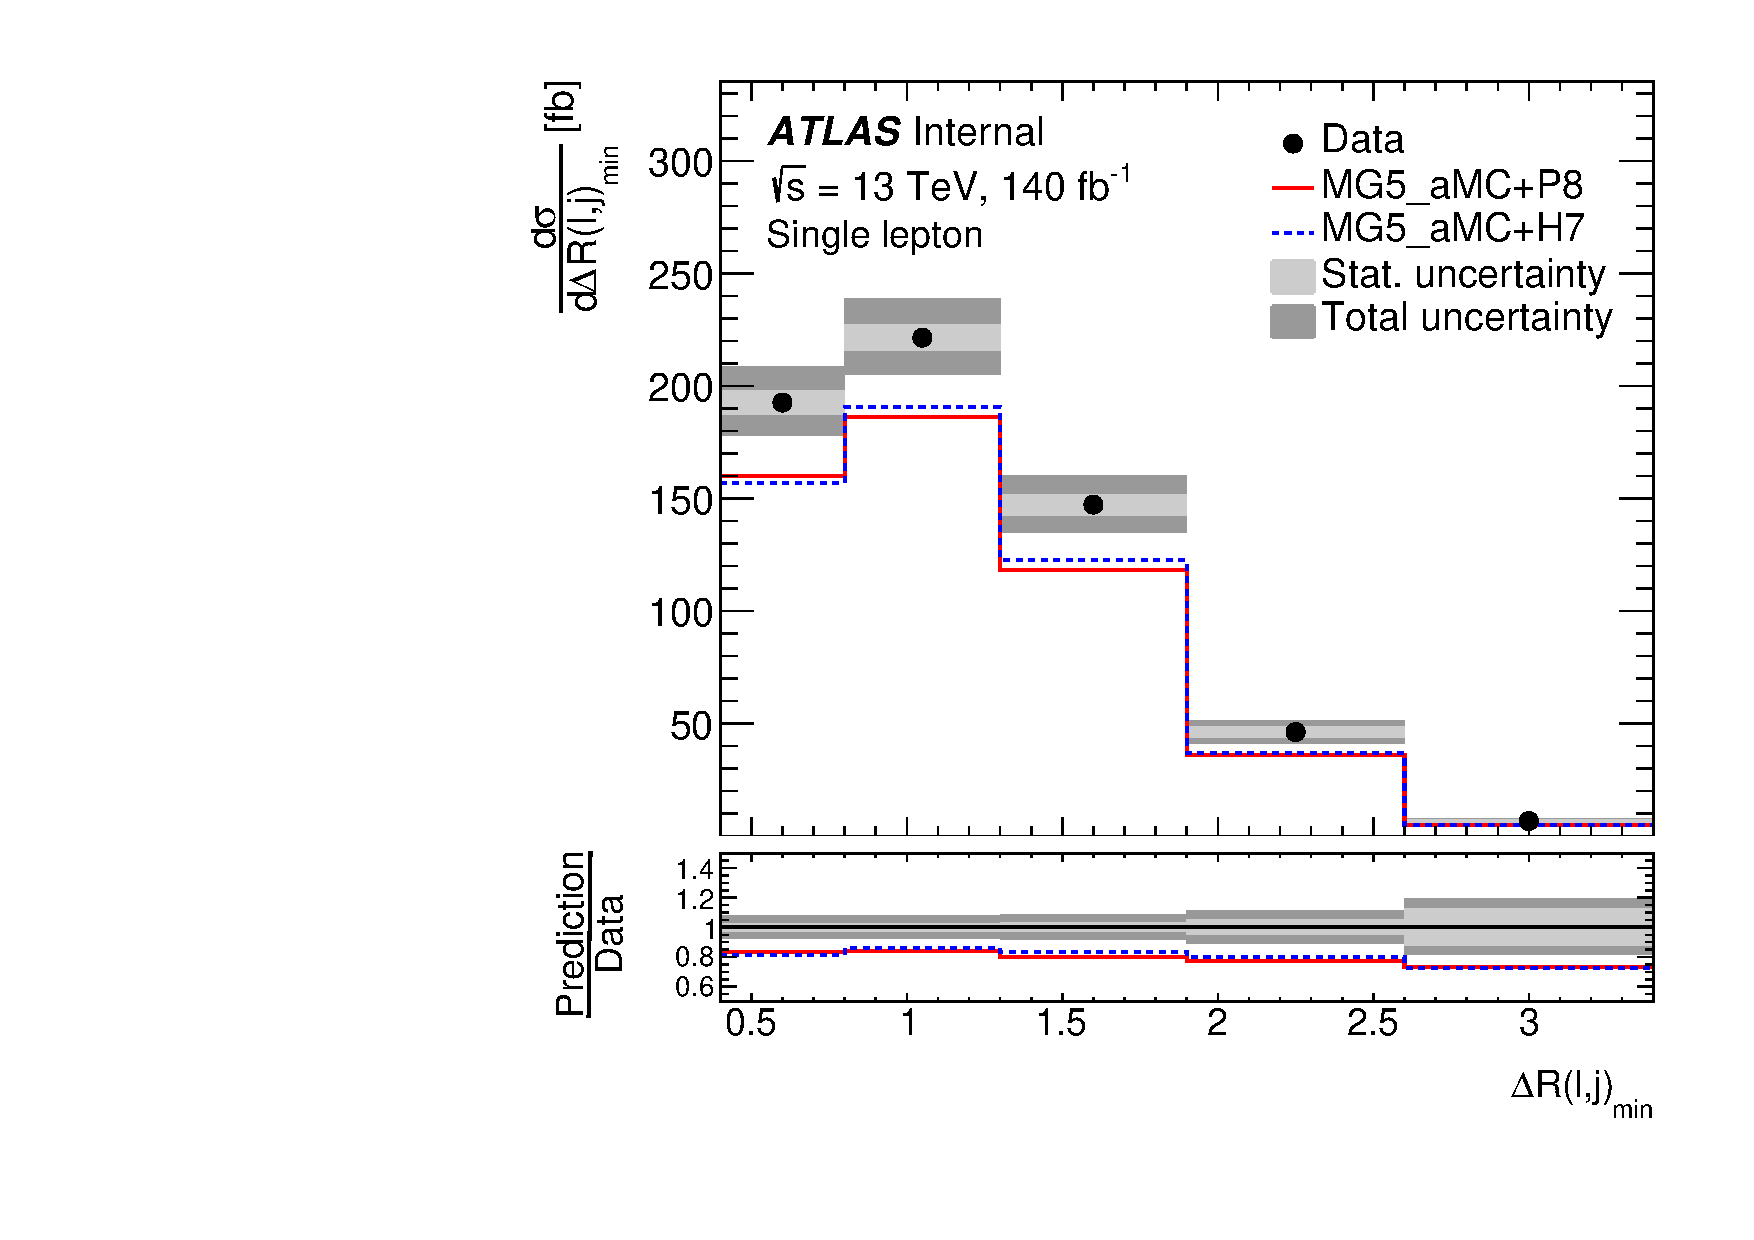
\includegraphics[width=0.4\textwidth]{figures/diff_xsec/absolute-unfolded-distributions/tty_prod_ljet/SL_tty_prod_drlj_unfolded_absolute.pdf}}
  \quad\quad
  \subfloat[]{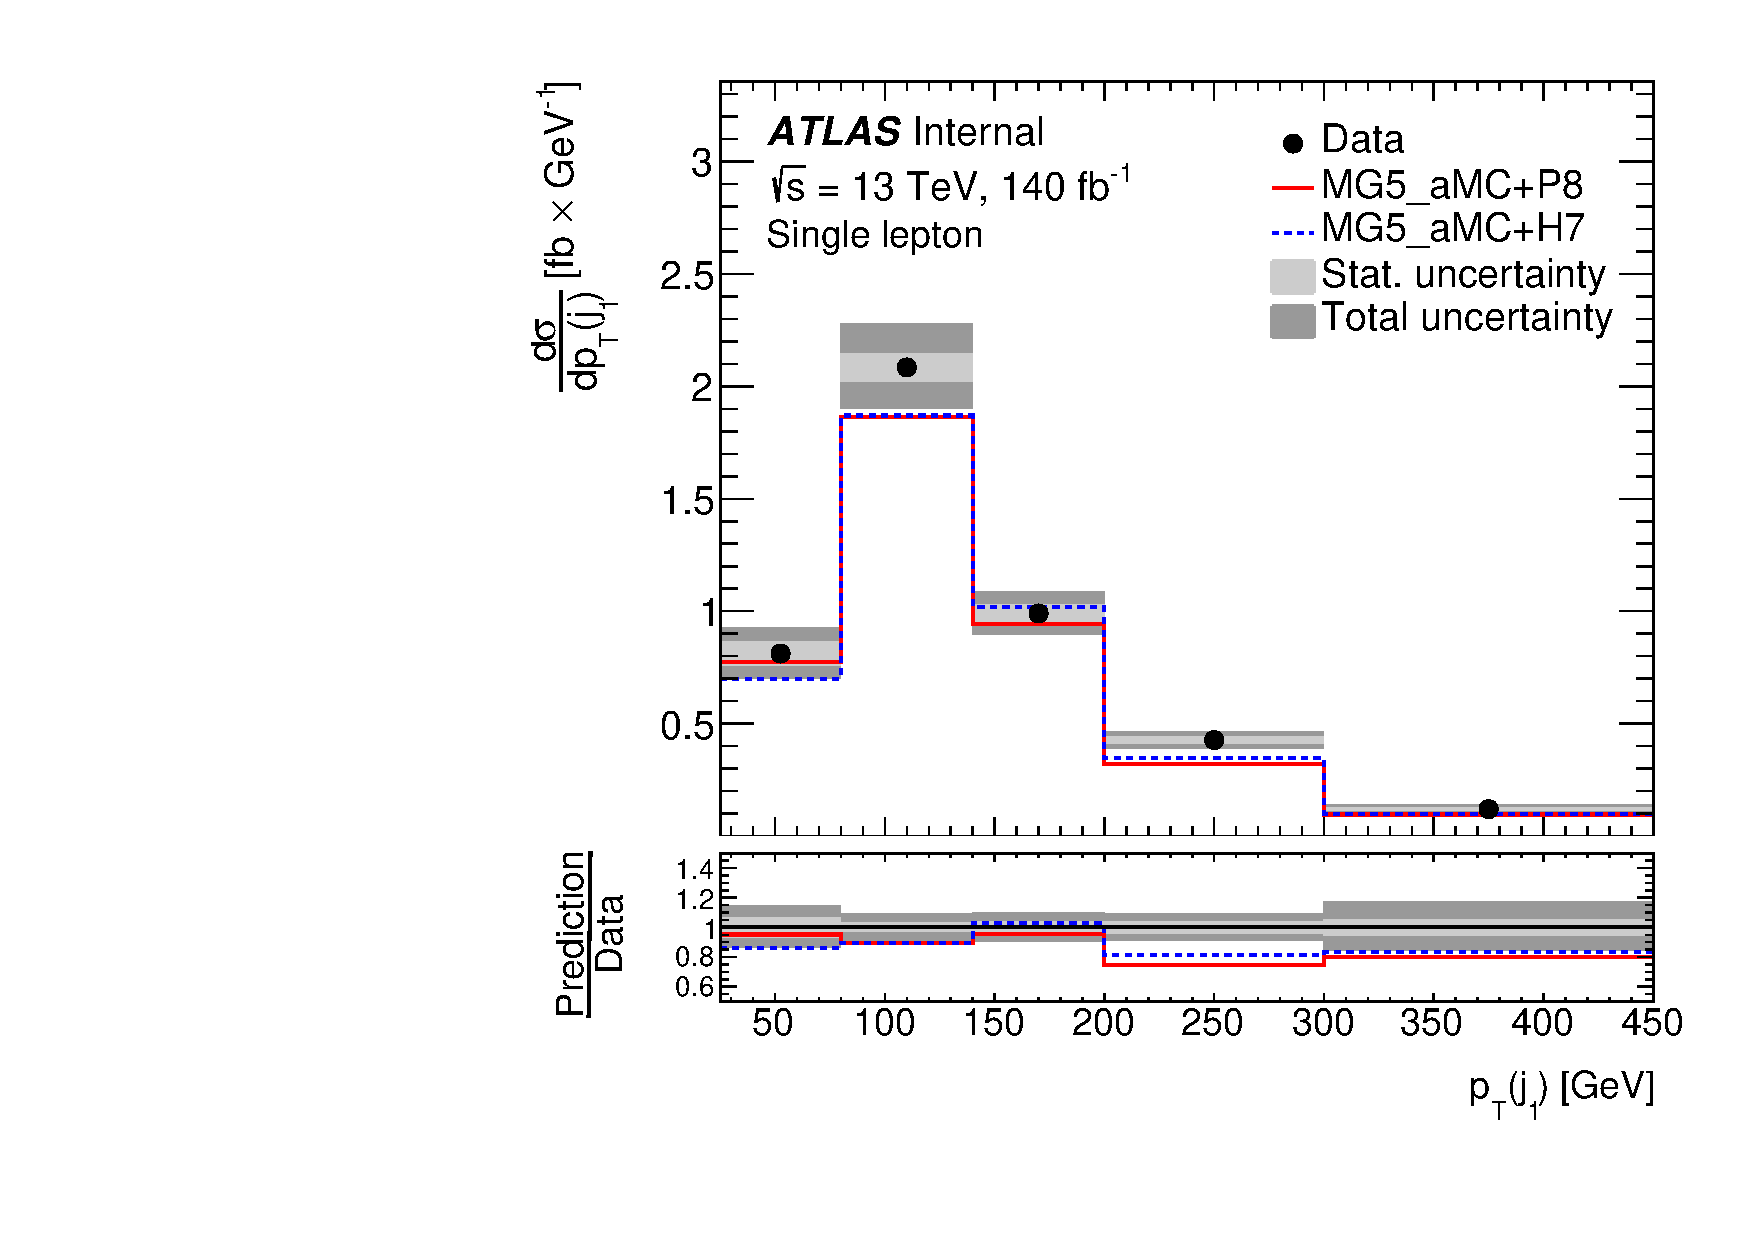
\includegraphics[width=0.4\textwidth]{figures/diff_xsec/absolute-unfolded-distributions/tty_prod_ljet/SL_tty_prod_ptj1_unfolded_absolute.pdf}}
  \quad\quad
  \caption{The particle-level unfolded distributions in the single lepton channel after fitting to the real dataset. 
  The error bars represent both statistical and systematic uncertainties. (a) $p_T(\gamma)$, (b) $|\eta(\gamma|)$, 
  (c) $\Delta R_{min}(\gamma, l)$, (d) $\Delta R(\gamma, b)$, (e) $\Delta R_{min}(l, j)$, (f) $p_T(j1)$. Overflow events are included in the last bin of the corresponding distribution.}
  \label{fig:pt_unfolded_ljet_dist_realdata}
\end{figure}
\FloatBarrier



\begin{figure}[ht]
  \centering
  \subfloat[]{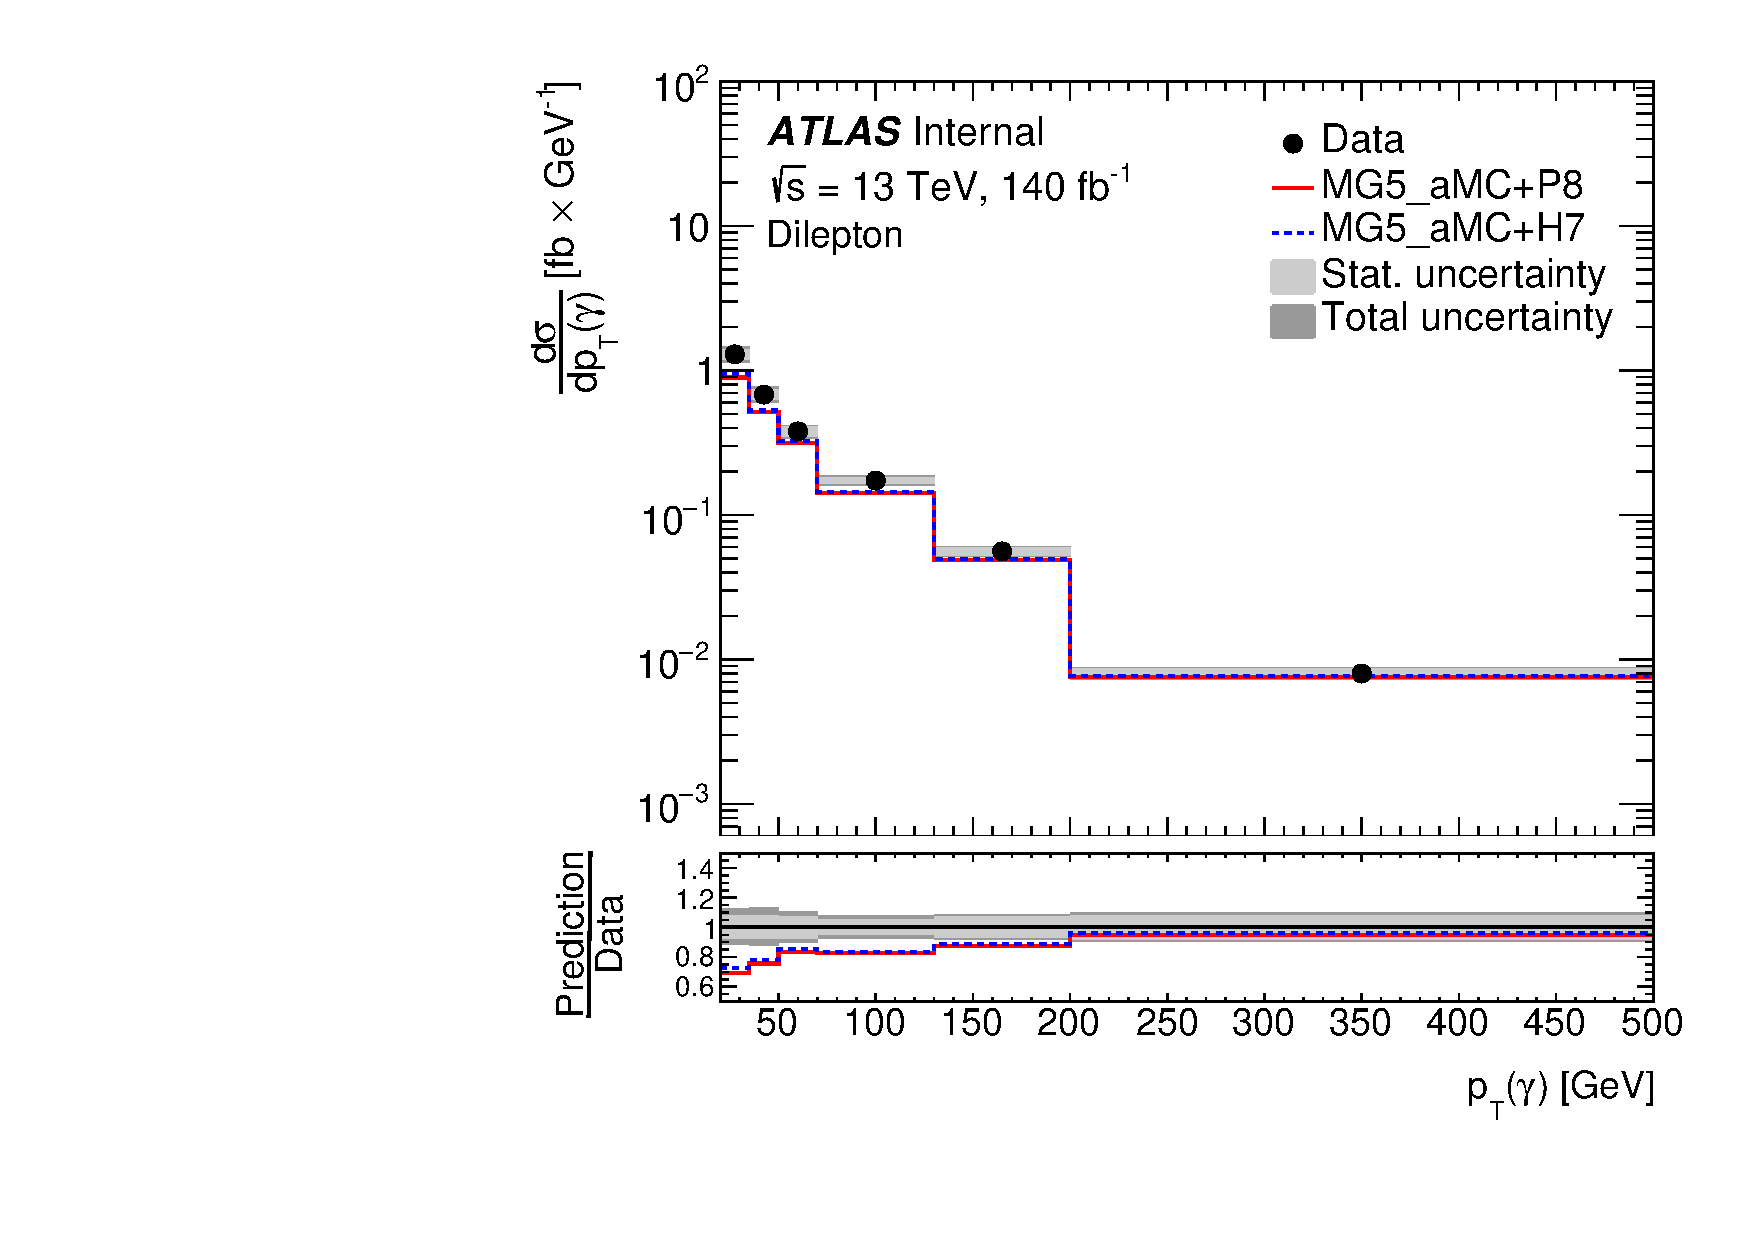
\includegraphics[width=0.4\textwidth]{figures/diff_xsec/absolute-unfolded-distributions/tty_prod_dilep/DL_tty_prod_pt_unfolded_absolute.pdf}}
  \quad\quad
  \subfloat[]{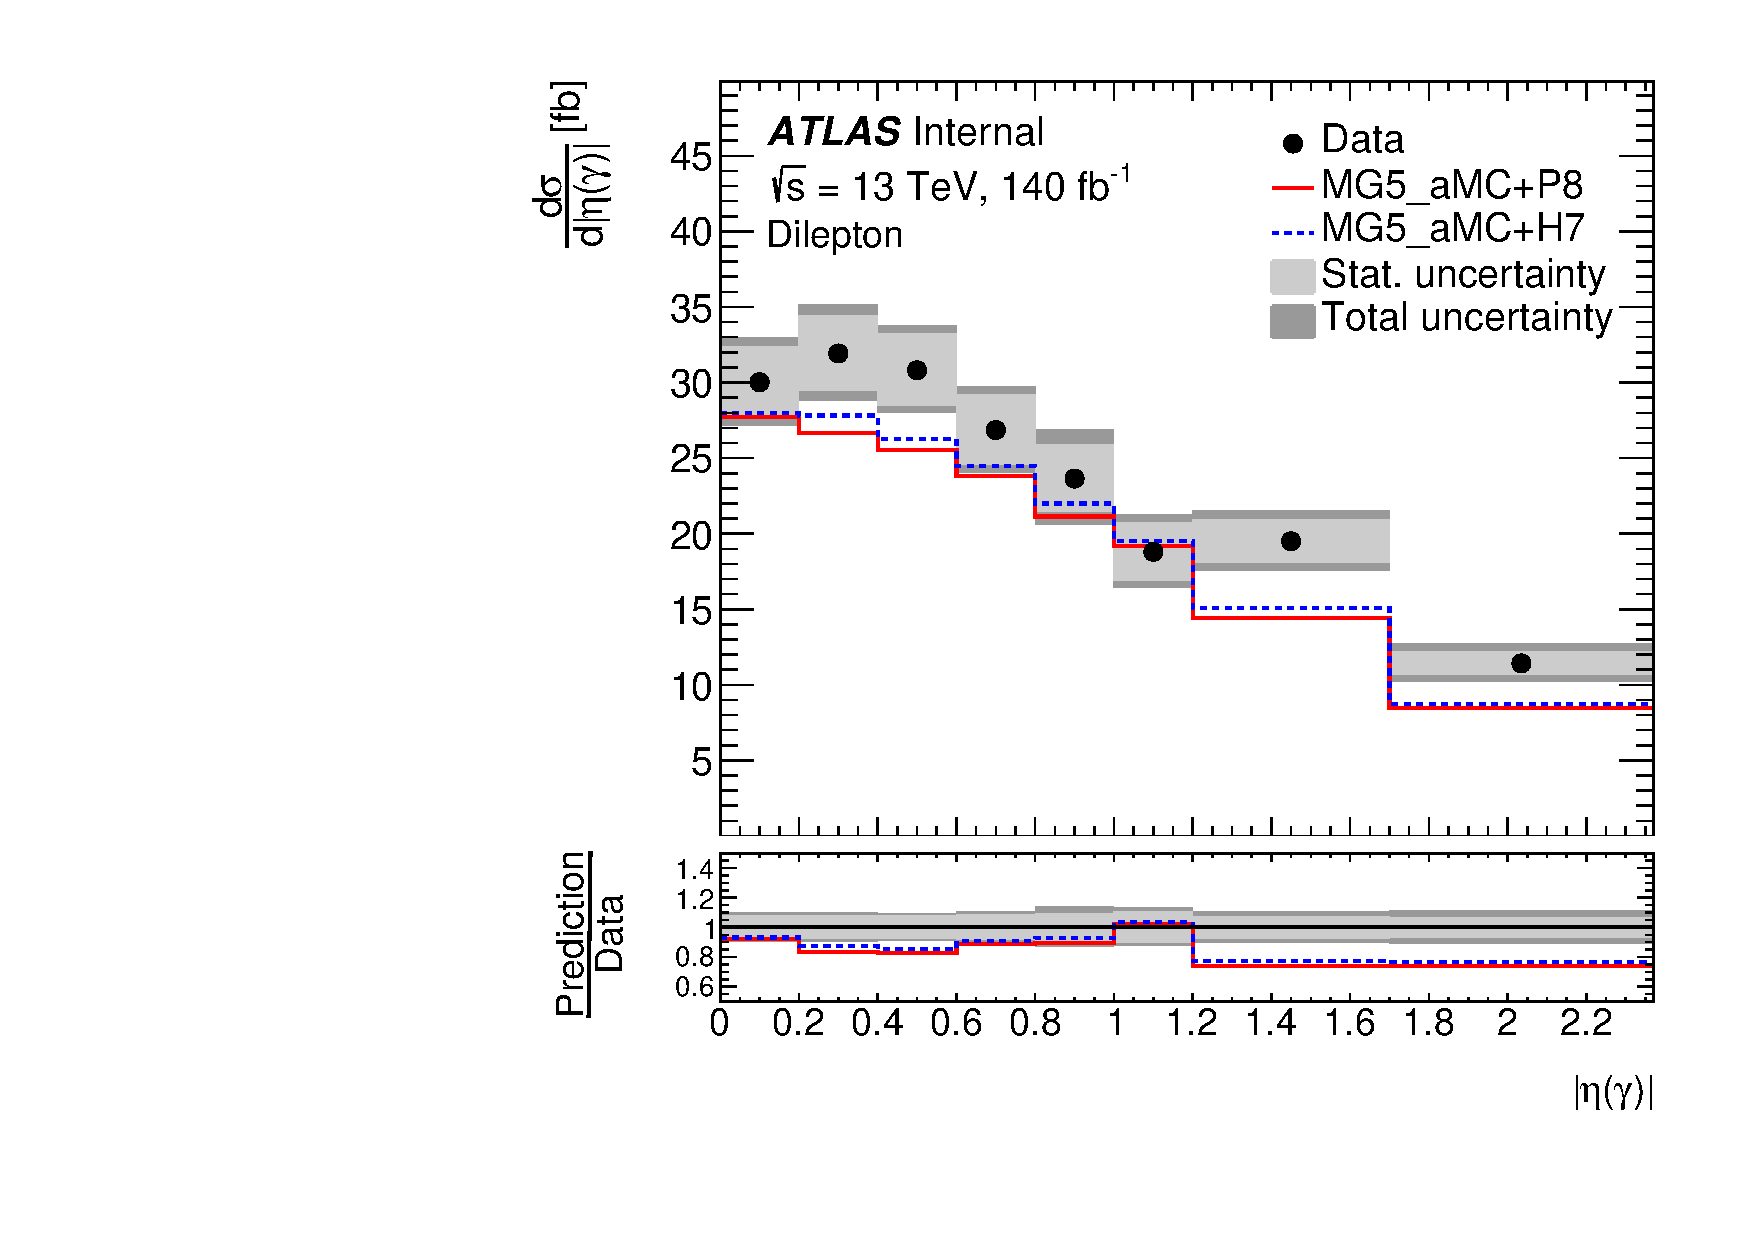
\includegraphics[width=0.4\textwidth]{figures/diff_xsec/absolute-unfolded-distributions/tty_prod_dilep/DL_tty_prod_eta_unfolded_absolute.pdf}}
  \quad\quad
  \subfloat[]{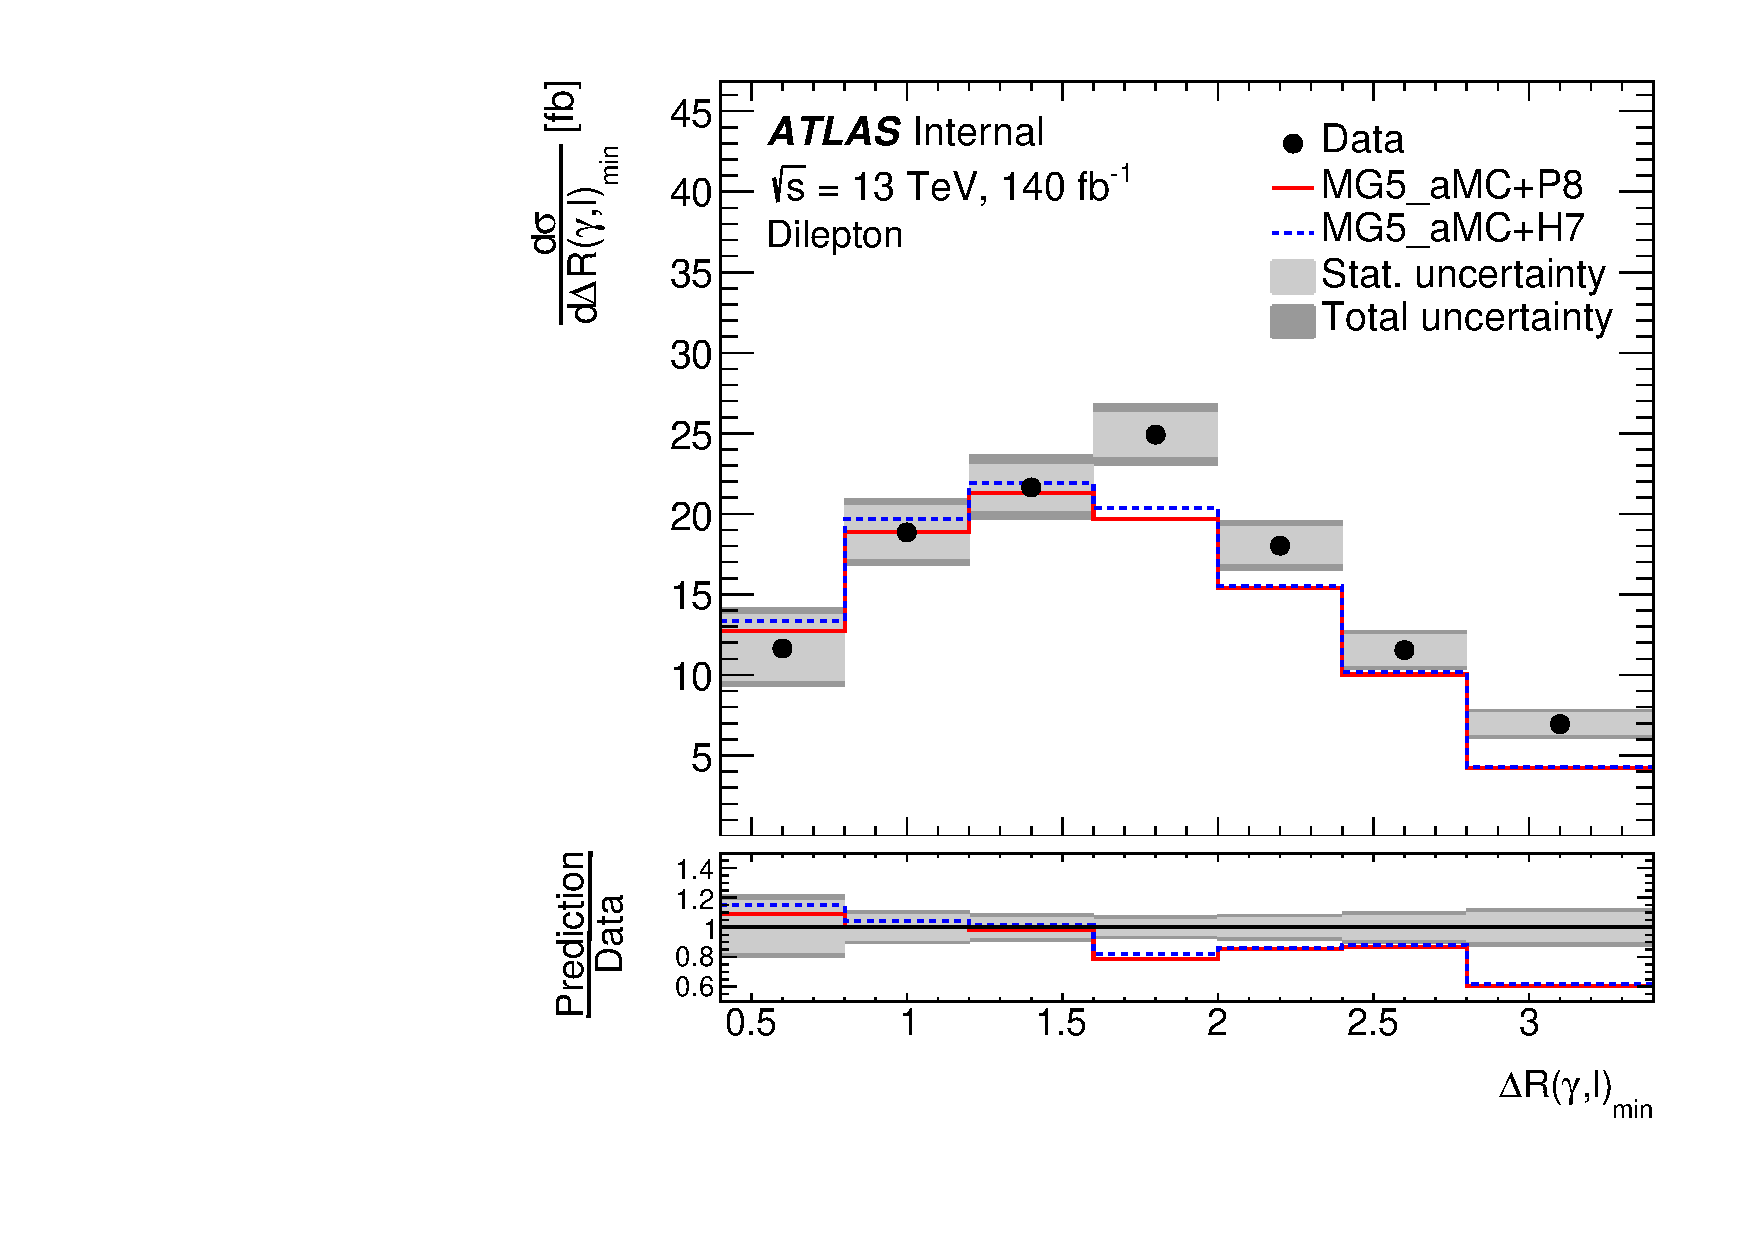
\includegraphics[width=0.4\textwidth]{figures/diff_xsec/absolute-unfolded-distributions/tty_prod_dilep/DL_tty_prod_drphl_unfolded_absolute.pdf}}
  \quad\quad
  \subfloat[]{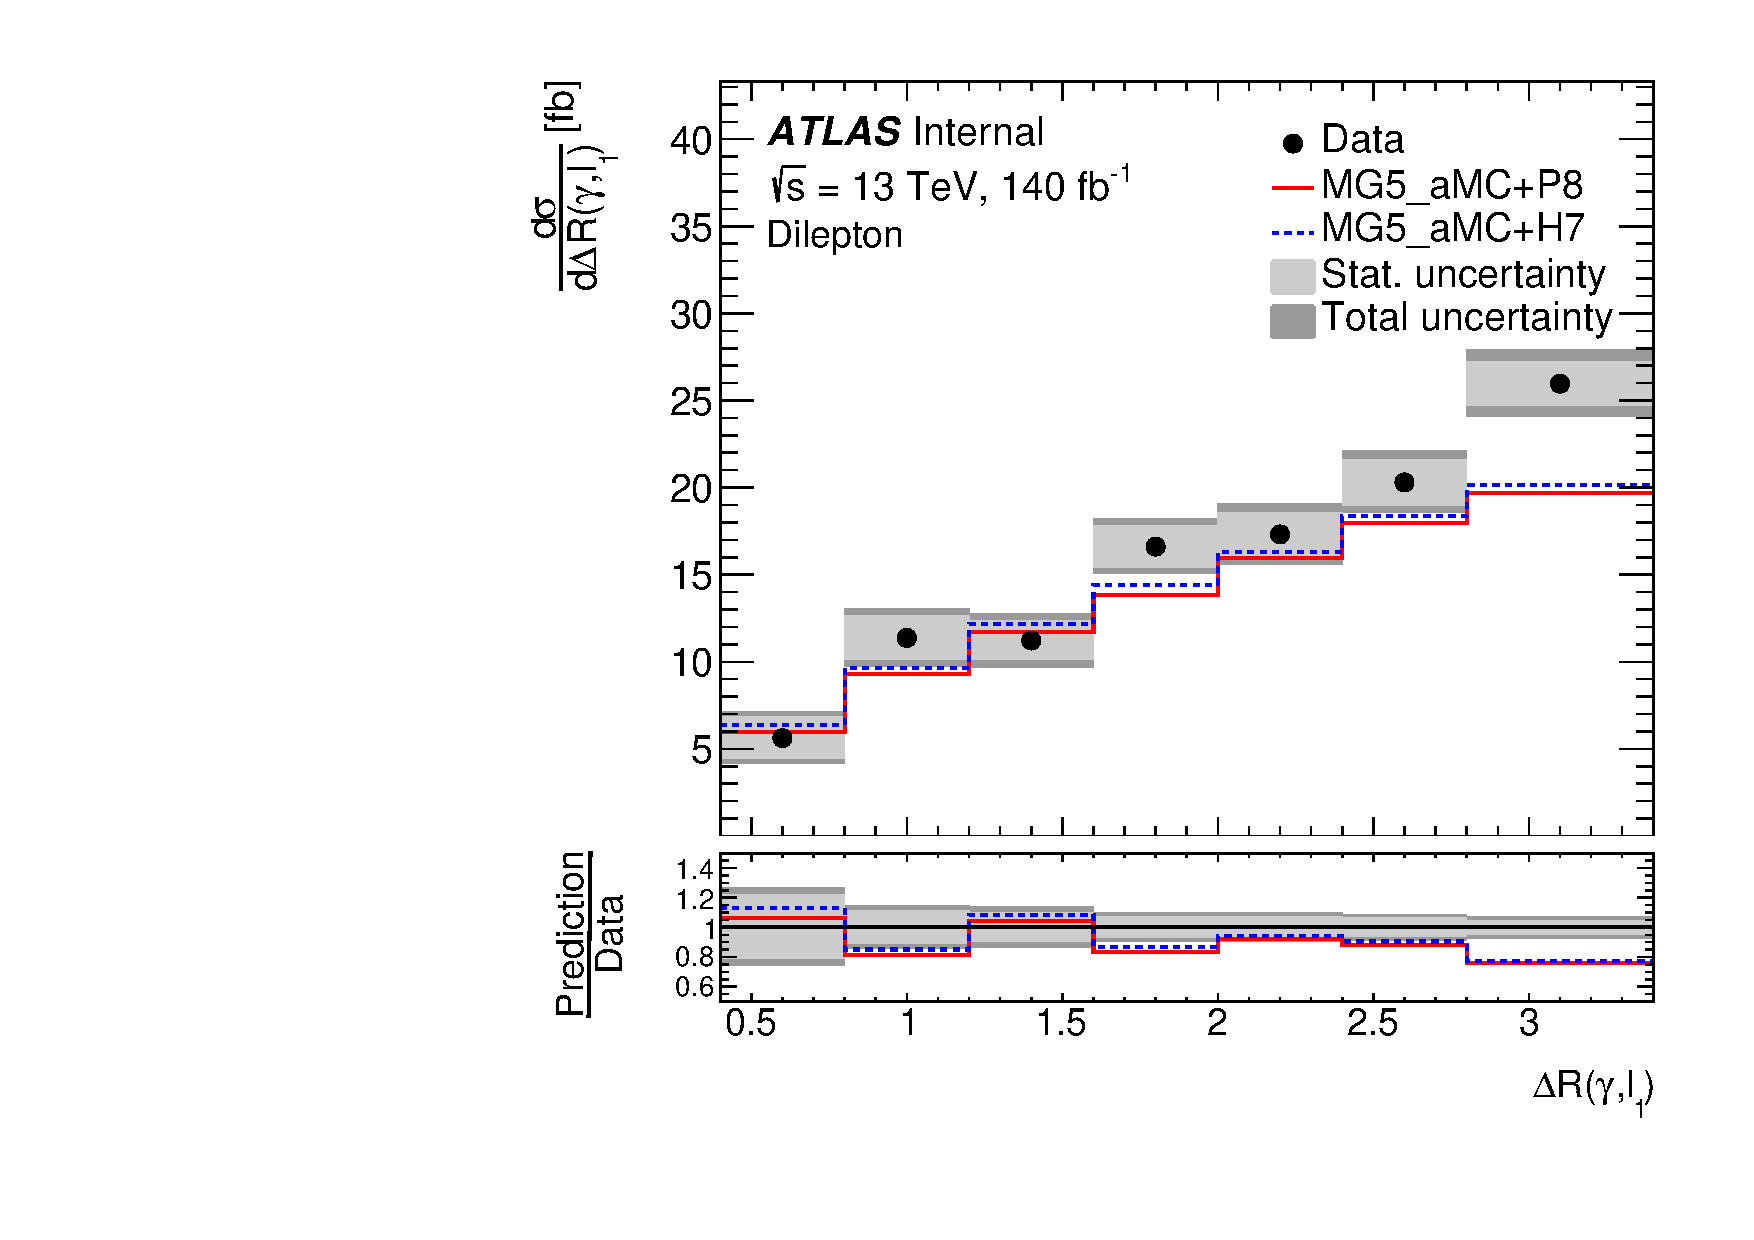
\includegraphics[width=0.4\textwidth]{figures/diff_xsec/absolute-unfolded-distributions/tty_prod_dilep/DL_tty_prod_drphl1_unfolded_absolute.pdf}}
  \quad\quad
  \subfloat[]{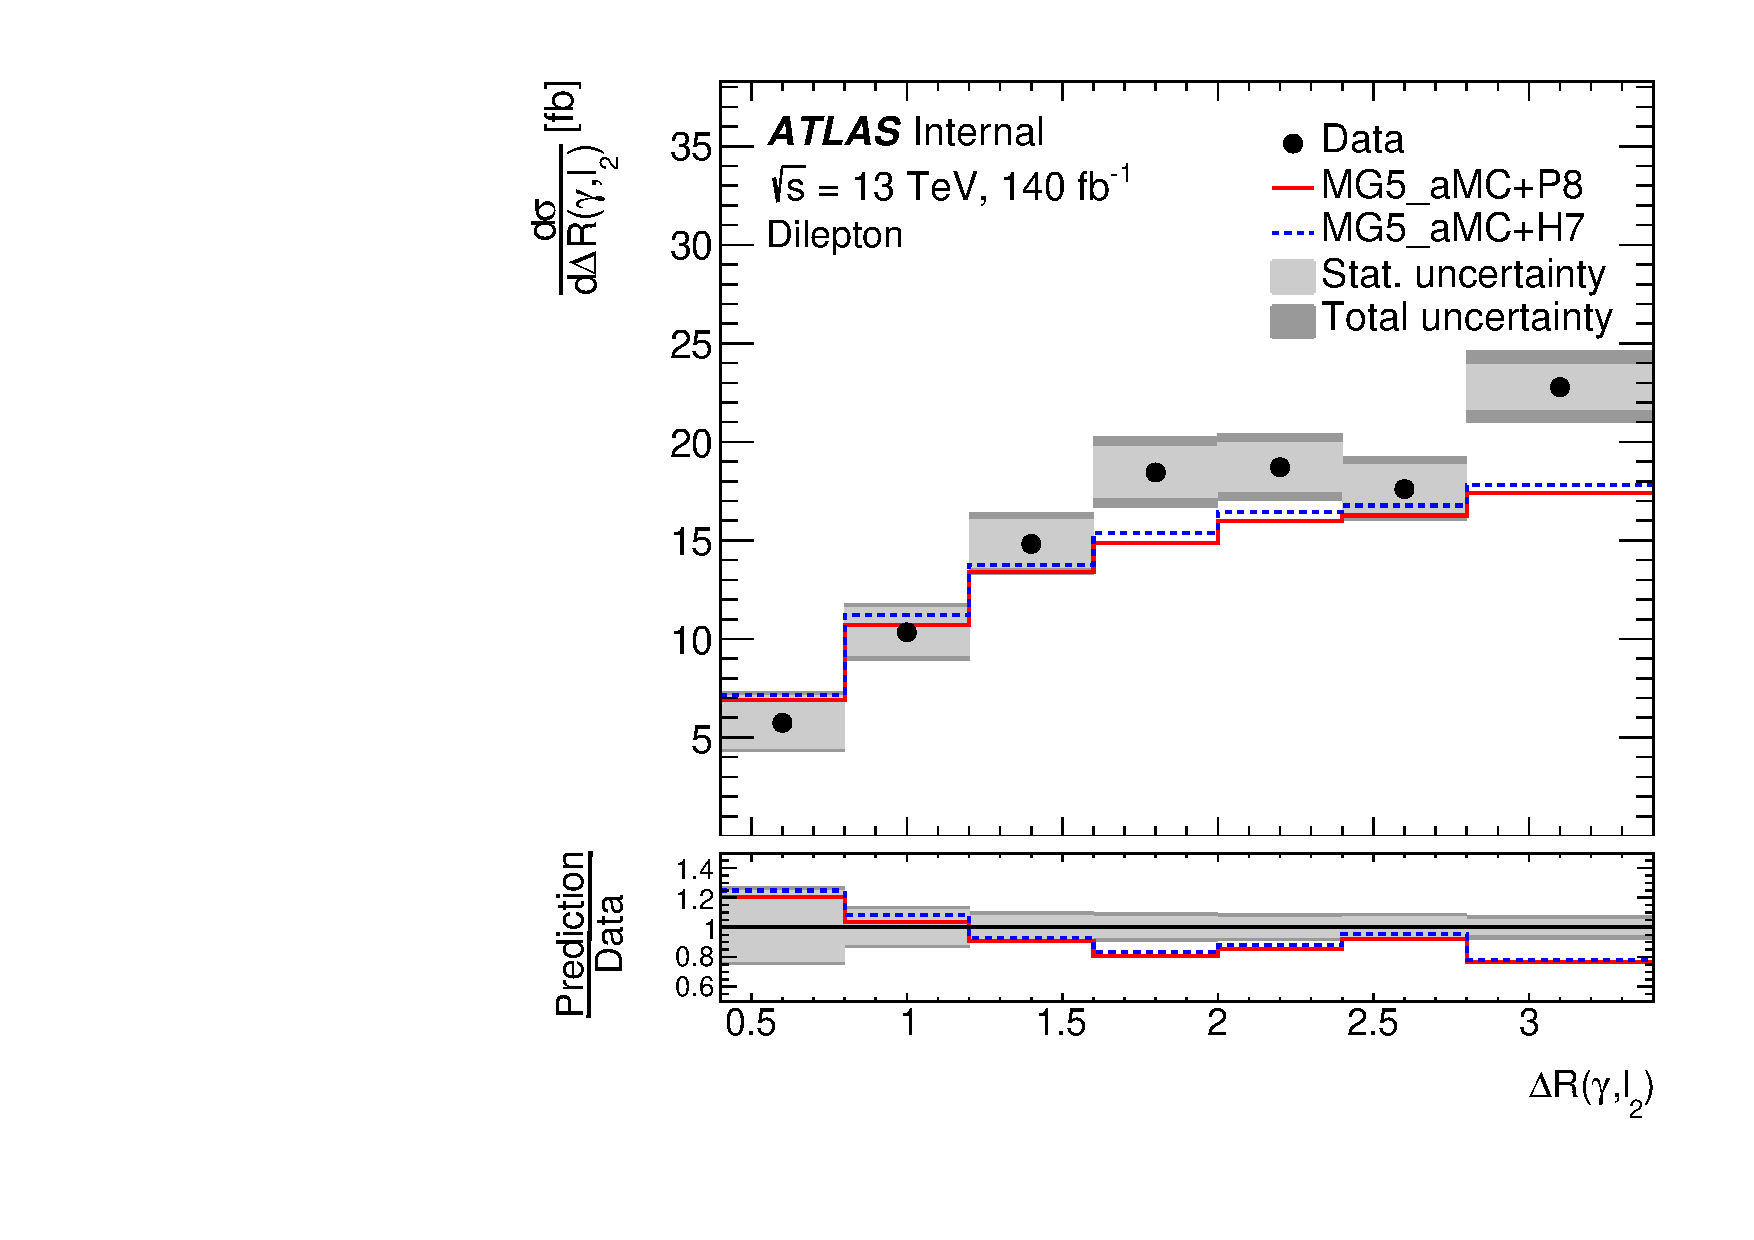
\includegraphics[width=0.4\textwidth]{figures/diff_xsec/absolute-unfolded-distributions/tty_prod_dilep/DL_tty_prod_drphl2_unfolded_absolute.pdf}}
  \quad\quad
  \subfloat[]{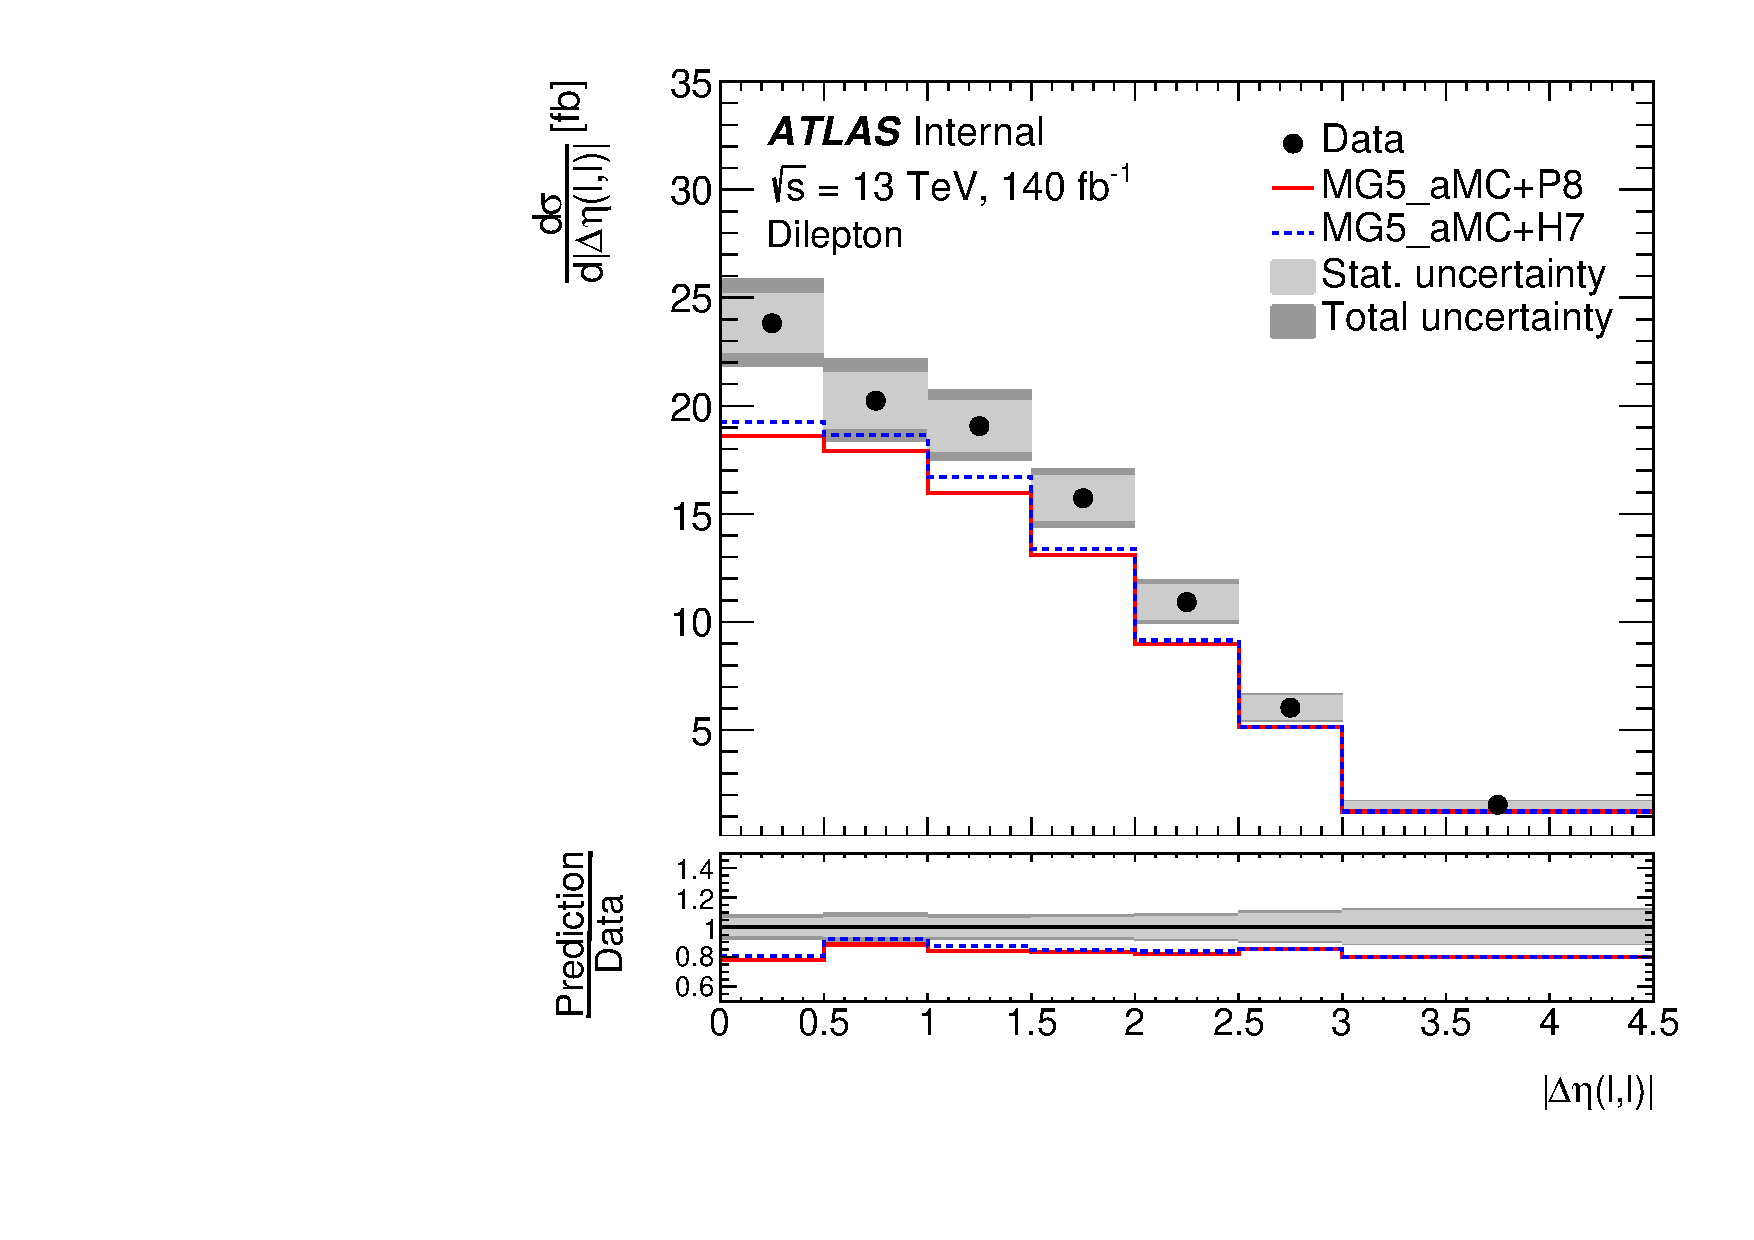
\includegraphics[width=0.4\textwidth]{figures/diff_xsec/absolute-unfolded-distributions/tty_prod_dilep/DL_tty_prod_dEtall_unfolded_absolute.pdf}}
  \caption{The particle-level unfolded distributions in the dilepton channel after fitting to the real dataset. 
  The error bars represent both statistical and systematic uncertainties. Overflow events are included in the last bin of the corresponding distribution.}
  \label{fig:pt_unfolded_dilep_dist_realdata_1}

\end{figure}

\begin{figure}[ht]
  \centering
  \subfloat[]{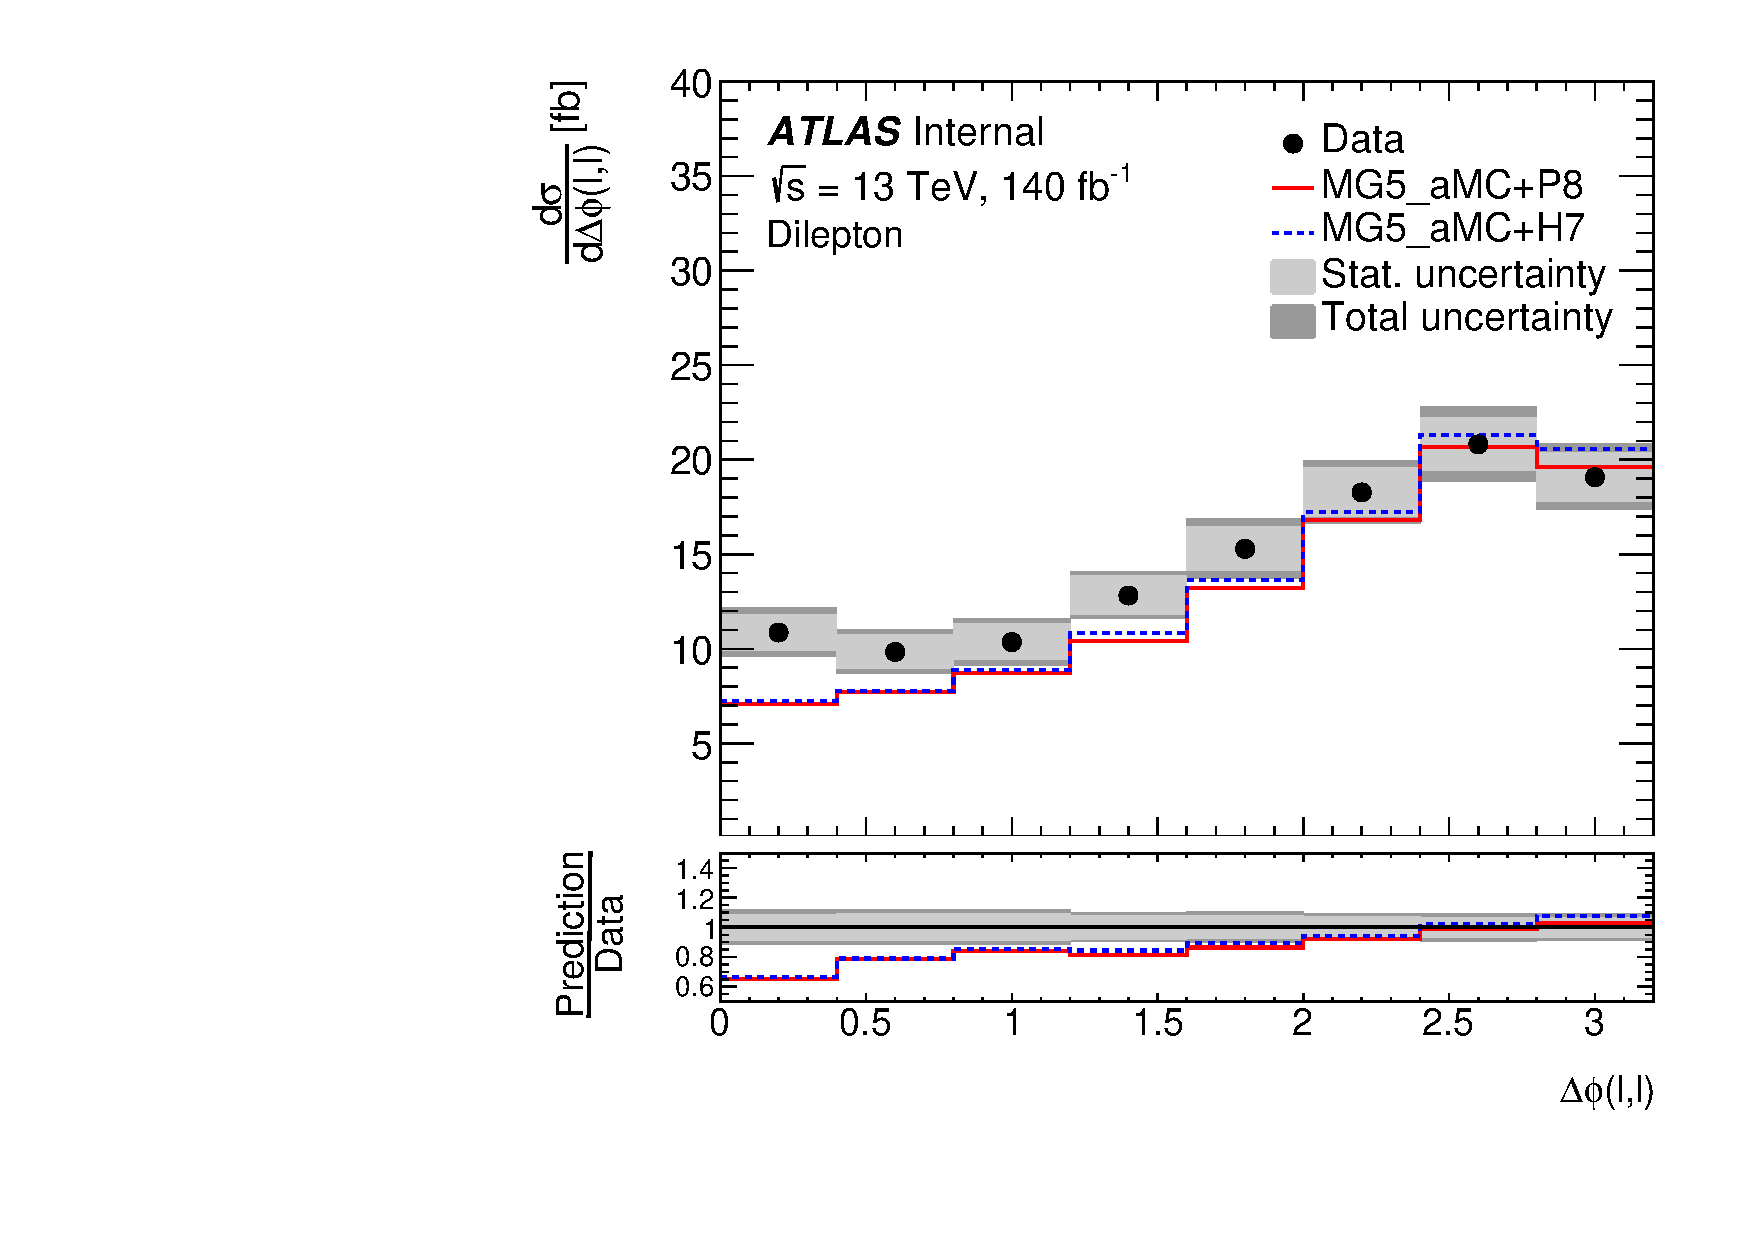
\includegraphics[width=0.4\textwidth]{figures/diff_xsec/absolute-unfolded-distributions/tty_prod_dilep/DL_tty_prod_dPhill_unfolded_absolute.pdf}}
  \quad\quad
  \subfloat[]{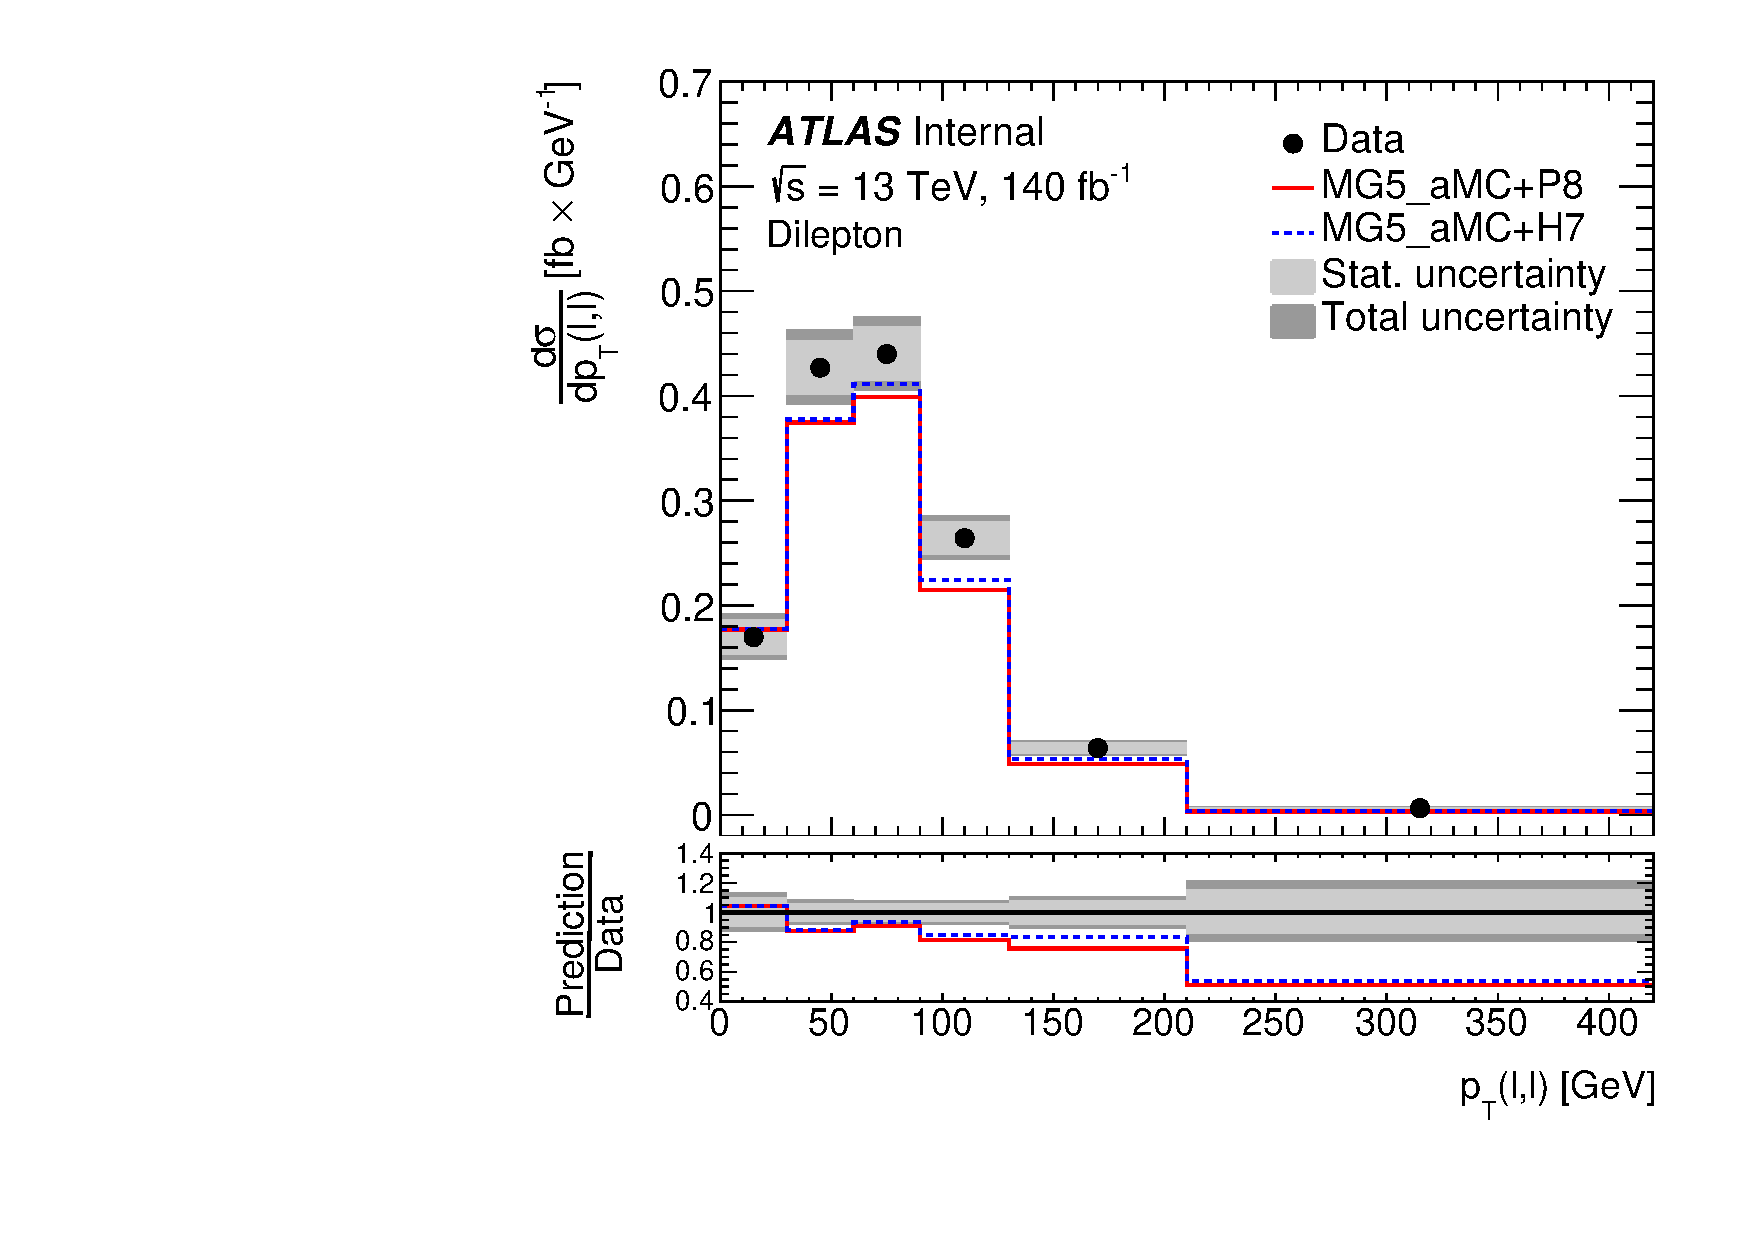
\includegraphics[width=0.4\textwidth]{figures/diff_xsec/absolute-unfolded-distributions/tty_prod_dilep/DL_tty_prod_ptll_unfolded_absolute.pdf}}
  \quad\quad
  \subfloat[]{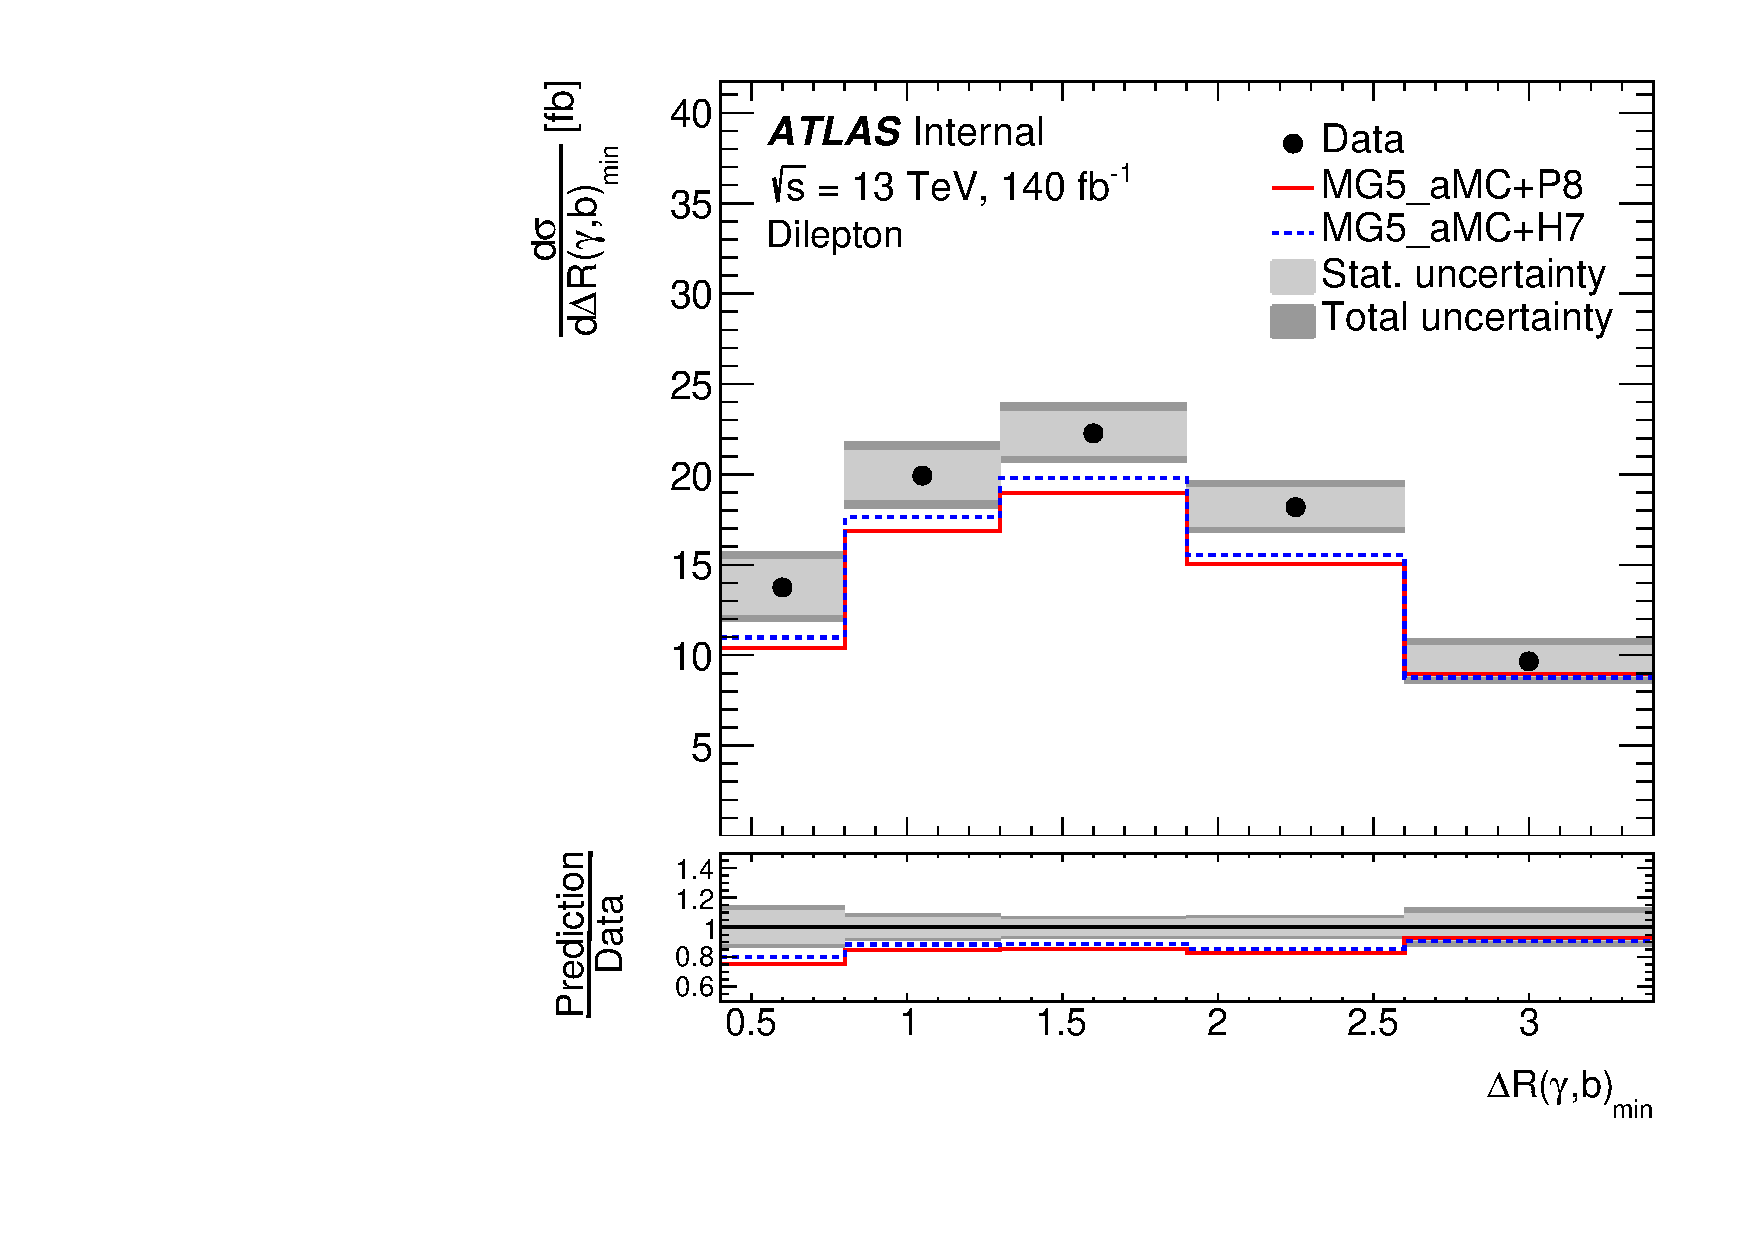
\includegraphics[width=0.4\textwidth]{figures/diff_xsec/absolute-unfolded-distributions/tty_prod_dilep/DL_tty_prod_drphb_unfolded_absolute.pdf}}
  \quad\quad
  \subfloat[]{\includegraphics[width=0.4\textwidth]{figures/diff_xsec/absolute-unfolded-distributions/tty_prod_dilep/DL_tty_prod_drlj_unfolded_absolute.pdf}}
  \quad\quad
  \subfloat[]{\includegraphics[width=0.4\textwidth]{figures/diff_xsec/absolute-unfolded-distributions/tty_prod_dilep/DL_tty_prod_ptj1_unfolded_absolute.pdf}}
  \quad\quad
\caption{The particle-level unfolded distributions in the dilepton channel after fitting to the real dataset. 
  The error bars represent both statistical and systematic uncertainties. Overflow events are included in the last bin of the corresponding distribution.}
  \label{fig:pt_unfolded_dilep_dist_realdata_2}
\end{figure}
\FloatBarrier


\begin{figure}[ht]
  \centering
  \subfloat[]{\includegraphics[width=0.3\textwidth]{figures/diff_xsec/ljet_tty_prod_mu_blinded/Unfolded_data/tty1l_pt_all_syst/NormFactors.pdf}}
  \quad
  \subfloat[]{\includegraphics[width=0.3\textwidth]{figures/diff_xsec/ljet_tty_prod_mu_blinded/Unfolded_data/tty1l_eta_all_syst/NormFactors.pdf}}
  \quad
  \subfloat[]{\includegraphics[width=0.3\textwidth]{figures/diff_xsec/ljet_tty_prod_mu_blinded/Unfolded_data/tty1l_dr_all_syst/NormFactors.pdf}}
  \quad
  \subfloat[]{\includegraphics[width=0.3\textwidth]{figures/diff_xsec/ljet_tty_prod_mu_blinded/Unfolded_data/tty1l_drphb_all_syst/NormFactors.pdf}}
  \quad
  \subfloat[]{\includegraphics[width=0.3\textwidth]{figures/diff_xsec/ljet_tty_prod_mu_blinded/Unfolded_data/tty1l_drlj_all_syst/NormFactors.pdf}}
  \quad
  \subfloat[]{\includegraphics[width=0.3\textwidth]{figures/diff_xsec/ljet_tty_prod_mu_blinded/Unfolded_data/tty1l_ptj1_all_syst/NormFactors.pdf}}
  \caption{ The figure displays the normalization factors obtained from the fit to the real dataset for the single 
  lepton channel for the following observables: (a) $p_T(\gamma)$, (b) $|\eta(\gamma|)$, 
  (c) $\Delta R_{min}(\gamma, l)$, (d) $\Delta R(\gamma, b)$, (e) $\Delta R_{min}(l, j)$, (f) $p_T(j1)$.}
  \label{fig:pt_unfolded_ljet_table_realdata}
\end{figure}
\FloatBarrier


\begin{figure}[ht]
  \centering
  \subfloat[]{\includegraphics[width=0.3\textwidth]{figures/diff_xsec/dilep_tty_prod_mu_blinded/Unfolded_data/tty2l_pt_all_syst/NormFactors.pdf}}
  \quad
  \subfloat[]{\includegraphics[width=0.3\textwidth]{figures/diff_xsec/dilep_tty_prod_mu_blinded/Unfolded_data/tty2l_eta_all_syst/NormFactors.pdf}}
  \quad
  \subfloat[]{\includegraphics[width=0.3\textwidth]{figures/diff_xsec/dilep_tty_prod_mu_blinded/Unfolded_data/tty2l_dr_all_syst/NormFactors.pdf}}
  \quad
  \subfloat[]{\includegraphics[width=0.3\textwidth]{figures/diff_xsec/dilep_tty_prod_mu_blinded/Unfolded_data/tty2l_dr1_all_syst/NormFactors.pdf}}
  \quad
  \subfloat[]{\includegraphics[width=0.3\textwidth]{figures/diff_xsec/dilep_tty_prod_mu_blinded/Unfolded_data/tty2l_dr2_all_syst/NormFactors.pdf}}
  \quad
  \subfloat[]{\includegraphics[width=0.3\textwidth]{figures/diff_xsec/dilep_tty_prod_mu_blinded/Unfolded_data/tty2l_dEtall_all_syst/NormFactors.pdf}}
  \quad
  \subfloat[]{\includegraphics[width=0.3\textwidth]{figures/diff_xsec/dilep_tty_prod_mu_blinded/Unfolded_data/tty2l_dPhill_all_syst/NormFactors.pdf}}
  \quad
  \subfloat[]{\includegraphics[width=0.3\textwidth]{figures/diff_xsec/dilep_tty_prod_mu_blinded/Unfolded_data/tty2l_ptll_all_syst/NormFactors.pdf}}
  \quad
  \subfloat[]{\includegraphics[width=0.3\textwidth]{figures/diff_xsec/dilep_tty_prod_mu_blinded/Unfolded_data/tty2l_drphb_all_syst/NormFactors.pdf}}
  \quad
  \subfloat[]{\includegraphics[width=0.3\textwidth]{figures/diff_xsec/dilep_tty_prod_mu_blinded/Unfolded_data/tty2l_drlj_all_syst/NormFactors.pdf}}
  \quad
  \subfloat[]{\includegraphics[width=0.3\textwidth]{figures/diff_xsec/dilep_tty_prod_mu_blinded/Unfolded_data/tty2l_ptj1_all_syst/NormFactors.pdf}}
  \caption{ The figure displays the normalisation factors obtained from the fit to the real dataset for the dilepton channel
  for the following observables: (a) $p_T(\gamma)$, (b) $|\eta(\gamma|)$, (c) $\Delta R_{min}(\gamma, l)$
  (d) $\Delta R(\gamma, l1)$, (e) $\Delta R(\gamma, l2)$, (f) $|\Delta \eta(l, l)|$, (g) $|\Delta \phi(l, l)|$,
   (h) $p_T(ll)$, (i) $\Delta R(\gamma, b)$, (j) $\Delta R_{min}(l, j)$, (k) $p_T(j1)$.}
  \label{fig:pt_unfolded_dilep_table_realdata}
\end{figure}
\FloatBarrier

